\documentclass[10pt,t]{beamer}

\usetheme{lmtslides}
\usepackage{eso-pic}
\usepackage{graphicx}
\usepackage{times}
\usepackage[latin1]{inputenc}
\usepackage[amssymb]{SIunits}
\usepackage{amsmath,amssymb}
\usepackage{eurosym}
\usepackage{booktabs}
\usepackage{colortbl}
\usepackage{url}
\usepackage[absolute,overlay]{textpos}
\usepackage{graphicx}
\usepackage{mathtools}
\usepackage{pifont}
\usepackage{appendixnumberbeamer}
\usepackage{subcaption}
\usepackage{amssymb,amsmath,mleftright,mathtools}
\usepackage{cite}
\usepackage[T1]{fontenc}
\usepackage{hyperref}
\usepackage{amsmath,amssymb,amsfonts}
\usepackage{array,booktabs}
\usepackage{algorithm}
\usepackage{algpseudocode} 
\usepackage{algorithmicx}
\usepackage{listings}
\usepackage{textcomp}
\usepackage{url}
\usepackage{caption} 
\usepackage{tcolorbox}
\usepackage{empheq}
\usepackage{varwidth}
\usepackage{balance}
\usepackage{flushend} 
\usepackage{stfloats}
\usepackage{emoji}

% TikZ for diagrams
\usepackage{tikz}
\usetikzlibrary{arrows.meta,shapes,positioning}
\usetikzlibrary{calc,angles,quotes}

% --- Macro for drawing a 2D spherocylinder ---
\newcolumntype{M}[1]{>{\centering\arraybackslash}m{#1}}

\newcommand{\drawSpherocyl}[4]{
    \begin{scope}[shift={(#1)},rotate=#2]
        \draw[line width=1pt,rounded corners=6pt] (-#3 + #4,#4) -- (#3 - #4,#4);
        \draw[line width=1pt,rounded corners=6pt] (-#3 + #4,-#4) -- (#3 - #4,-#4);
        \draw[line width=1pt,rounded corners=6pt] (#3 - #4,-#4) arc[start angle=-90,end angle=90,radius=#4];
        \draw[line width=1pt,rounded corners=6pt] (-#3 + #4,#4) arc[start angle=90,end angle=270,radius=#4];
        \fill [black] (#1) circle (2pt);
    \end{scope}
}

\DeclareMathAlphabet\mathbfcal{OMS}{cmsy}{b}{n}

\setbeamertemplate{caption}{\raggedright\insertcaption\par}
\setbeamertemplate{bibliography item}[online]
\graphicspath{{figures/}}

\setlang{en}	

\newcommand{\xmark}{\ding{55}}%
\newcommand{\cmark}{\ding{51}}%

\renewcommand{\footnoterule}{\vfill\kern -3pt  \kern 2.6pt}

\setbeamertemplate{caption}{\raggedright\insertcaption\par}
\setbeamertemplate{bibliography item}[online]
\graphicspath{{figures/figures_paper/}}

\title{Proliferating Cell Collectives:\\ A Comparison of Hard and Soft Collision Models}
\type{Sf}
\author{Manuel Lerchner}
\email{manuel.lerchner@tum.de}
\advisorOne{Samuel James Newcome}
\advisorTwo{}
\date{\today}

\AtBeginSection[]
{
    \begin{frame}
        \frametitle{Outline}
        \tableofcontents[currentsection,currentsubsection]
    \end{frame}
}

\begin{document}

\maketitle

\setcounter{framenumber}{0}

% ============================================================
% SECTION 1: MOTIVATION & CONTEXT
% ============================================================

\section{Motivation}

\begin{frame}
    \frametitle{Computational Biology}

    \begin{columns}
        \begin{column}{0.58\textwidth}
            \textbf{Why simulate Bacteria?}
            \begin{itemize}
                \item Local rules $\to$ emergent behavior
                \item Test hypotheses in silico
                \item Beautiful visualizations
            \end{itemize}

            \vspace{0.5cm}

            \textbf{Computational challenge:}
            \begin{itemize}
                \item Large system sizes ($10^6$ cells)
                \item Complex interactions
                \item Long timescales
            \end{itemize}
        \end{column}

        \begin{column}{0.5\textwidth}
            \centering
            \begin{figure}
                \centering
                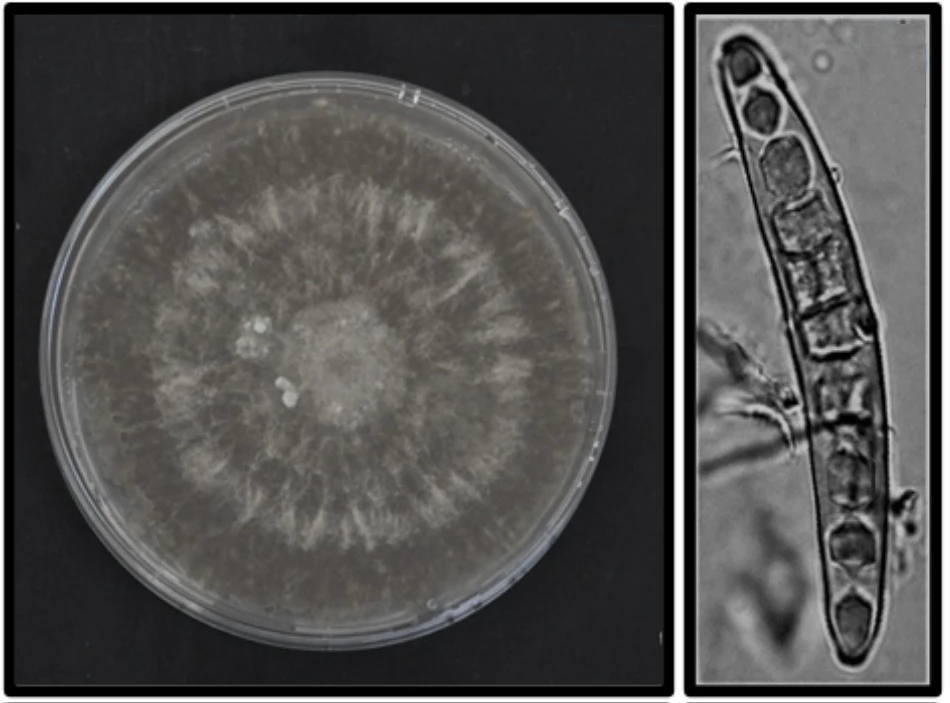
\includegraphics[width=\textwidth]{figures/figures_paper/real-bacteria/Exserohilum turcicum.png}
                \caption*{\scriptsize{Real fungal colony showing macroscopic ring patterns~\cite{Bankole2023}.}}
            \end{figure}
        \end{column}
    \end{columns}

\end{frame}


% \begin{frame}
%     \frametitle{The Performance Gap in Biological Modeling}

%     \begin{block}{Common Practice: Focus on Biological Insight}
%         \begin{itemize}
%             \item Pick a model that reproduces behavior
%             \item Validate against experimental patterns
%             \item Publish biological findings
%             \item \textbf{Runtime? Scaling? Source Code?} Often unreported
%         \end{itemize}
%     \end{block}

%     \vspace{0.1cm}

%     \begin{alertblock}{The Neglected Computational Core}
%         \begin{itemize}
%             \item \textbf{Efficiency:} Can we optimize further?
%             \item \textbf{Scaling:} How does it handle larger systems?
%             \item \textbf{Trade-offs:} What's the speed vs. accuracy balance?
%             \item \textbf{Comparisons:} Are different methods equivalent?
%         \end{itemize}
%     \end{alertblock}
% \end{frame}

\begin{frame}
    \frametitle{Small-scale: Simulating individual Bacteria}

    \vspace{0.3cm}

    \begin{columns}[c]
        \begin{column}{0.5\textwidth}
            \begin{figure}
                \centering
                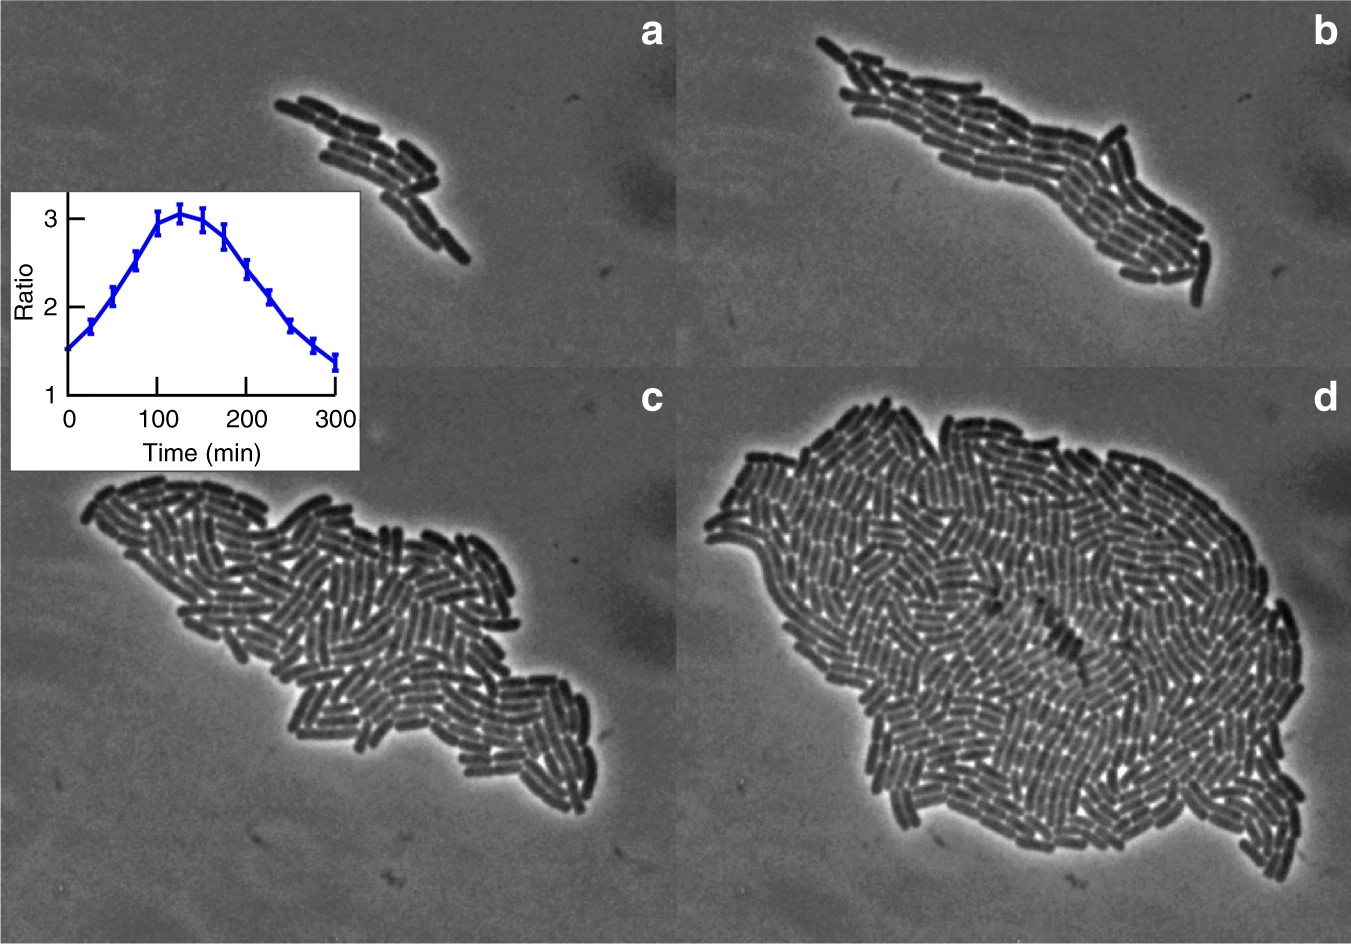
\includegraphics[width=1\textwidth]{figures/ecoli.png}
                \caption*{\scriptsize{E. coli colony \cite{DellArciprete2018}}}
            \end{figure}
        \end{column}

        \begin{column}{0.45\textwidth}
            \begin{tikzpicture}[node distance=2.8cm, auto]
                \tikzstyle{block} = [rectangle, draw, fill=blue!20,
                text width=6em, text centered,
                rounded corners, minimum height=1cm]
                \tikzstyle{arrow} = [thick,->,>=stealth]
                \tikzstyle{redarrow} = [line width=1.5pt, red, ->,>=stealth]

                \node [block] (growth) {Cell Growth and Division};
                \node [block, right of=growth] (collision) {Collisions};
                \node [block, below=1.2cm of collision] (stress) {Forces and Stress};
                \node [block, left of=stress] (inhibit) {Growth Inhibition};

                \draw [arrow] (growth) -- (collision);
                \draw [redarrow] (collision) -- (stress);
                \draw [arrow] (stress) -- (inhibit);
                \draw [arrow] (inhibit) -- (growth);
            \end{tikzpicture}
        \end{column}
    \end{columns}
\end{frame}

% ============================================================
% SECTION 3: MATHEMATICAL MODEL
% ============================================================

\section{Mathematical Framework}


\begin{frame}
    \frametitle{Cell Representation: Rigid Spherocylinders}

    \begin{figure}
        \centering
        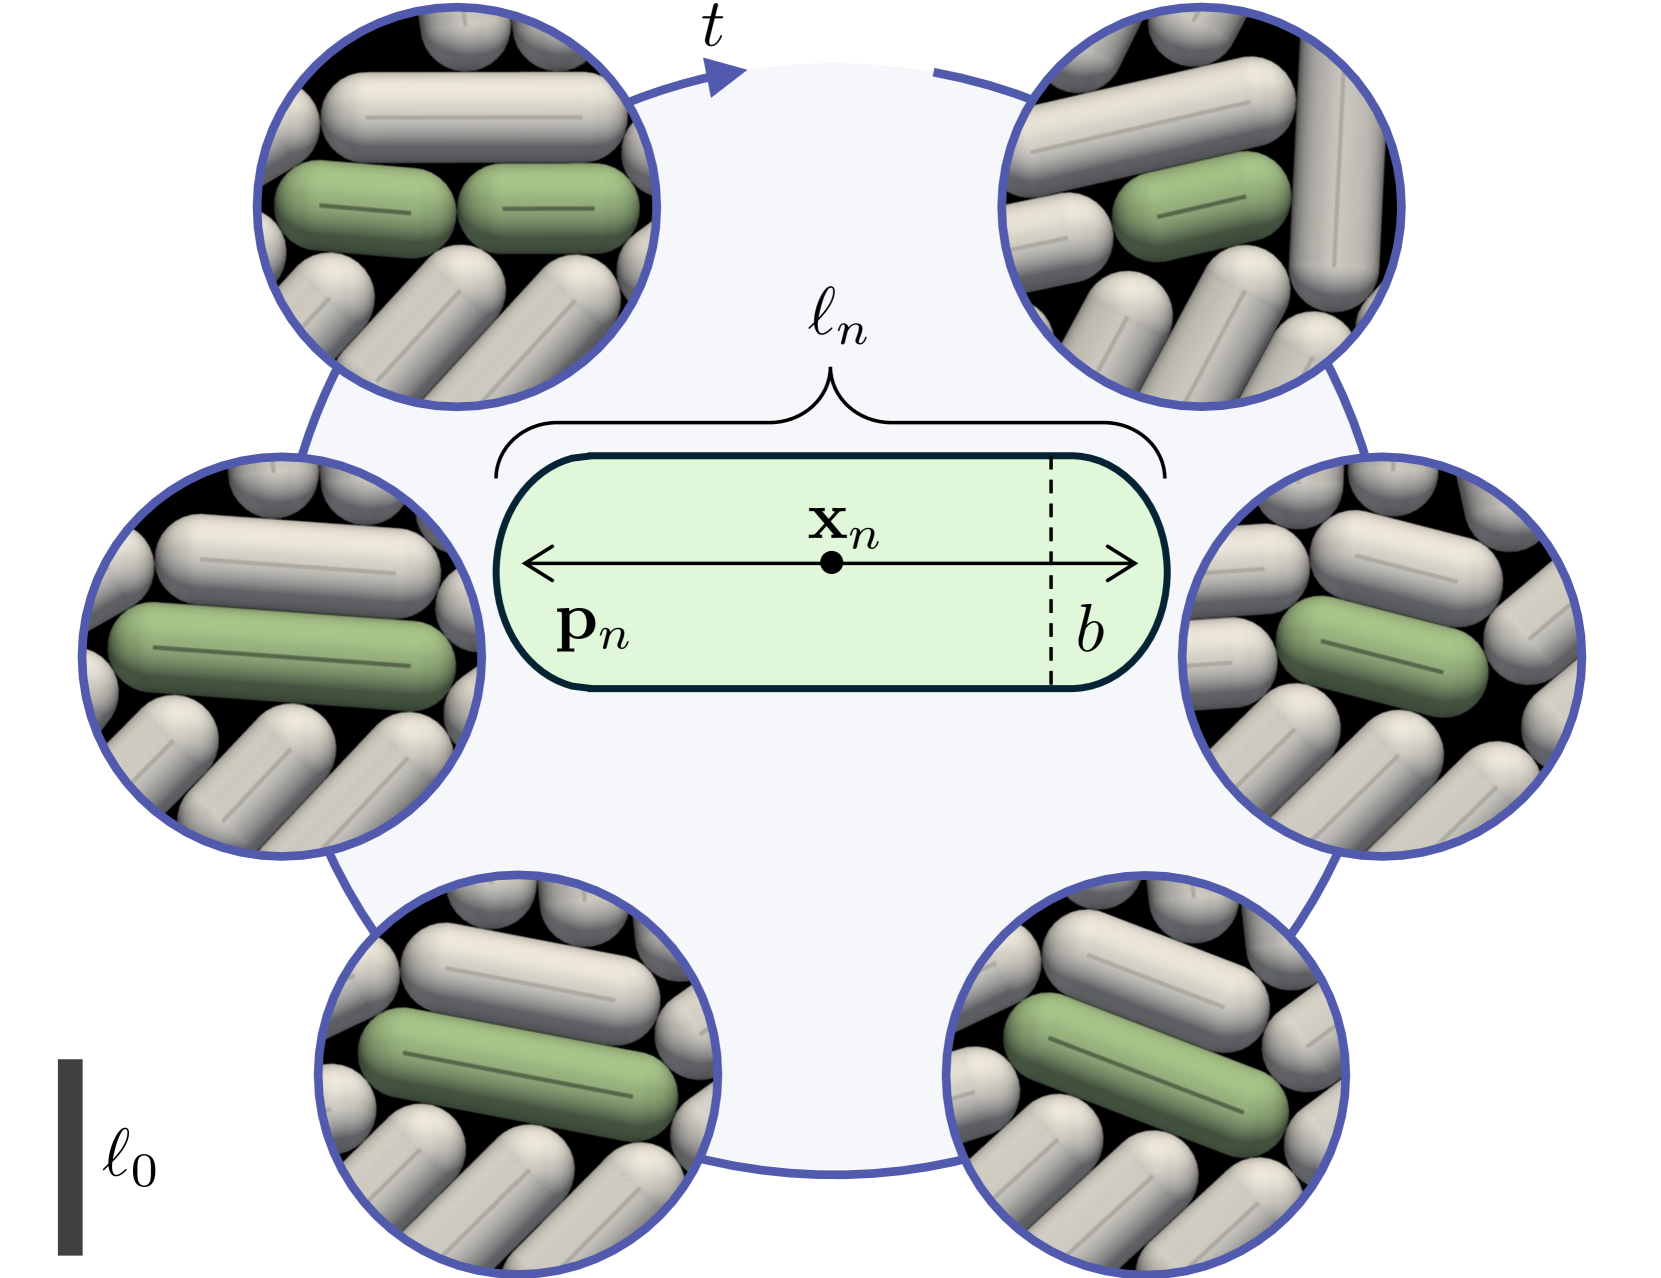
\includegraphics[width=0.65\textwidth]{figures/cell_model_weady.png}
        \caption*{\scriptsize{Spherocylindrical cell model~\cite{Weady2024}.}}
    \end{figure}

\end{frame}

\begin{frame}
    \frametitle{Cell Dynamics}

    \begin{columns}[c]
        \begin{column}{0.5\textwidth}

            \textbf{Overdamped dynamics:}
            \begin{itemize}
                \item Collision cause forces
                \item Inertia negligible
                \item Cells "swim in honey"
            \end{itemize}

            \vspace{0.5cm}

            \textbf{Equations of motion:}
            \begin{equation*}
                \begin{align}
                    \text{Translation:} \quad & \mathbf{u}_i = \frac{1}{\zeta \ell_i} \sum_{j \neq i} \mathbf{F}_{ij}                                    \\
                    \text{Rotation:} \qquad   & \boldsymbol{\omega}_i = \frac{12}{\zeta \ell_i^3} \sum_{j \neq i} \mathbf{r}_{ij} \times \mathbf{F}_{ij}
                \end{align}
            \end{equation*}
        \end{column}

        \begin{column}{0.35\textwidth}
            \vspace{-0.5cm}
            \begin{figure}
                \centering
                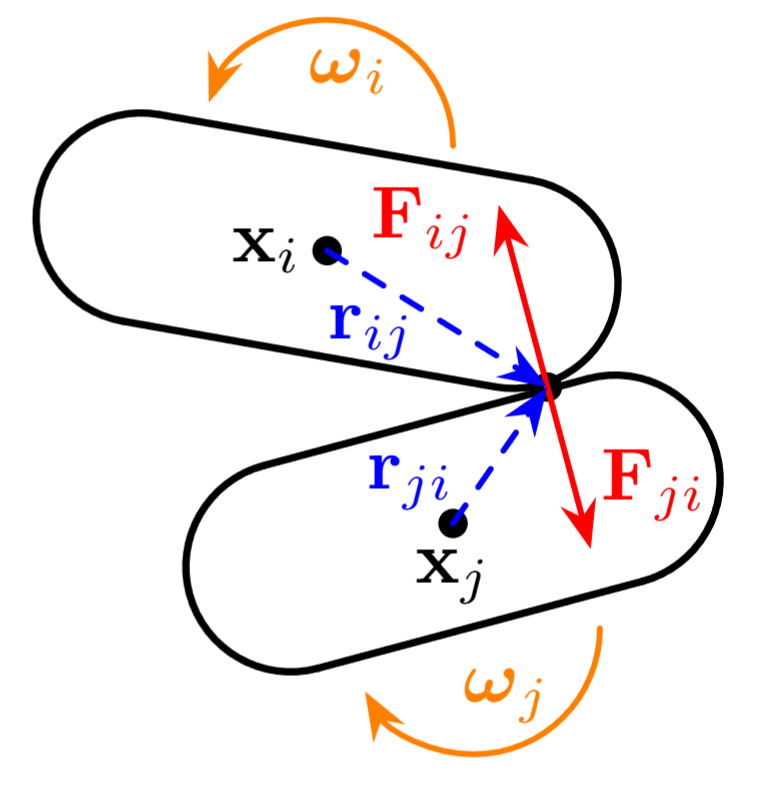
\includegraphics[width=1\textwidth]{figures/spherocylinder_model_collision.png}
            \end{figure}
        \end{column}
    \end{columns}

\end{frame}


\begin{frame}
    \frametitle{Cell Growth}

    \begin{columns}[c]
        \begin{column}{0.5\textwidth}

            \textbf{Stress-dependent growth:}
            \begin{itemize}
                \item Exponential growth
                \item Inhibited by longitudinal stress
            \end{itemize}

            \vspace{0.5cm}

            \textbf{Growth rate:}
            \begin{equation*}
                \begin{align}
                    \text{Growth rate: }   \quad & \dot{\ell}_i   = \frac{\ell_i}{\tau} e^{-\lambda \sigma_i}                                       \\
                    \text{Cell stress:} \qquad   & \sigma_i  = \sum_{j \neq i} \tfrac{1}{2} \left| \hat{\mathbf{t}}_i \cdot \mathbf{F}_{ij} \right|
                \end{align}
            \end{equation*}
        \end{column}

        \begin{column}{0.4\textwidth}
            \vspace{-0.5cm}
            \begin{tikzpicture}[line cap=round,line join=round,>=Stealth, scale=0.9]
                \coordinate (xi) at (0.8,-0.5);
                \coordinate (xj) at (2.68,-1.0);
                \def\R{0.5}

                \drawSpherocyl{xi}{-10}{1.4}{\R}
                \drawSpherocyl{xj}{60}{1.3}{\R}

                \coordinate (contact) at  (2.09,-0.92);
                \fill[black] (contact) circle (2pt) node[above right] {};

                \draw[->,thick,red] (contact) -- ++($.9*(-0.86,0.5)$) node[pos=1,below] {$\mathbf{F}_{ij}$};
                \draw[->,thick,red] (contact) -- ++($.9*(0.86,-0.5)$) node[pos=0.5,below] {$\mathbf{F}_{ji}$};

                \draw[->,thick,blue] (xi) -- ++($-0.8*(cos{-10},sin{-10})$) node[pos=1.2] {$\hat{\mathbf{t}}_i$};
                \draw[->,thick,blue] (xj) -- ++($0.8*(cos{60},sin{60})$) node[pos=1.2] {$\hat{\mathbf{t}}_j$};
            \end{tikzpicture}
        \end{column}
    \end{columns}

\end{frame}


% ============================================================
% SECTION 4: COLLISION MODELS
% ============================================================

\section{Collision Models}


\begin{frame}
    \frametitle{Collision Resolution}

    \begin{figure}
        \centering
        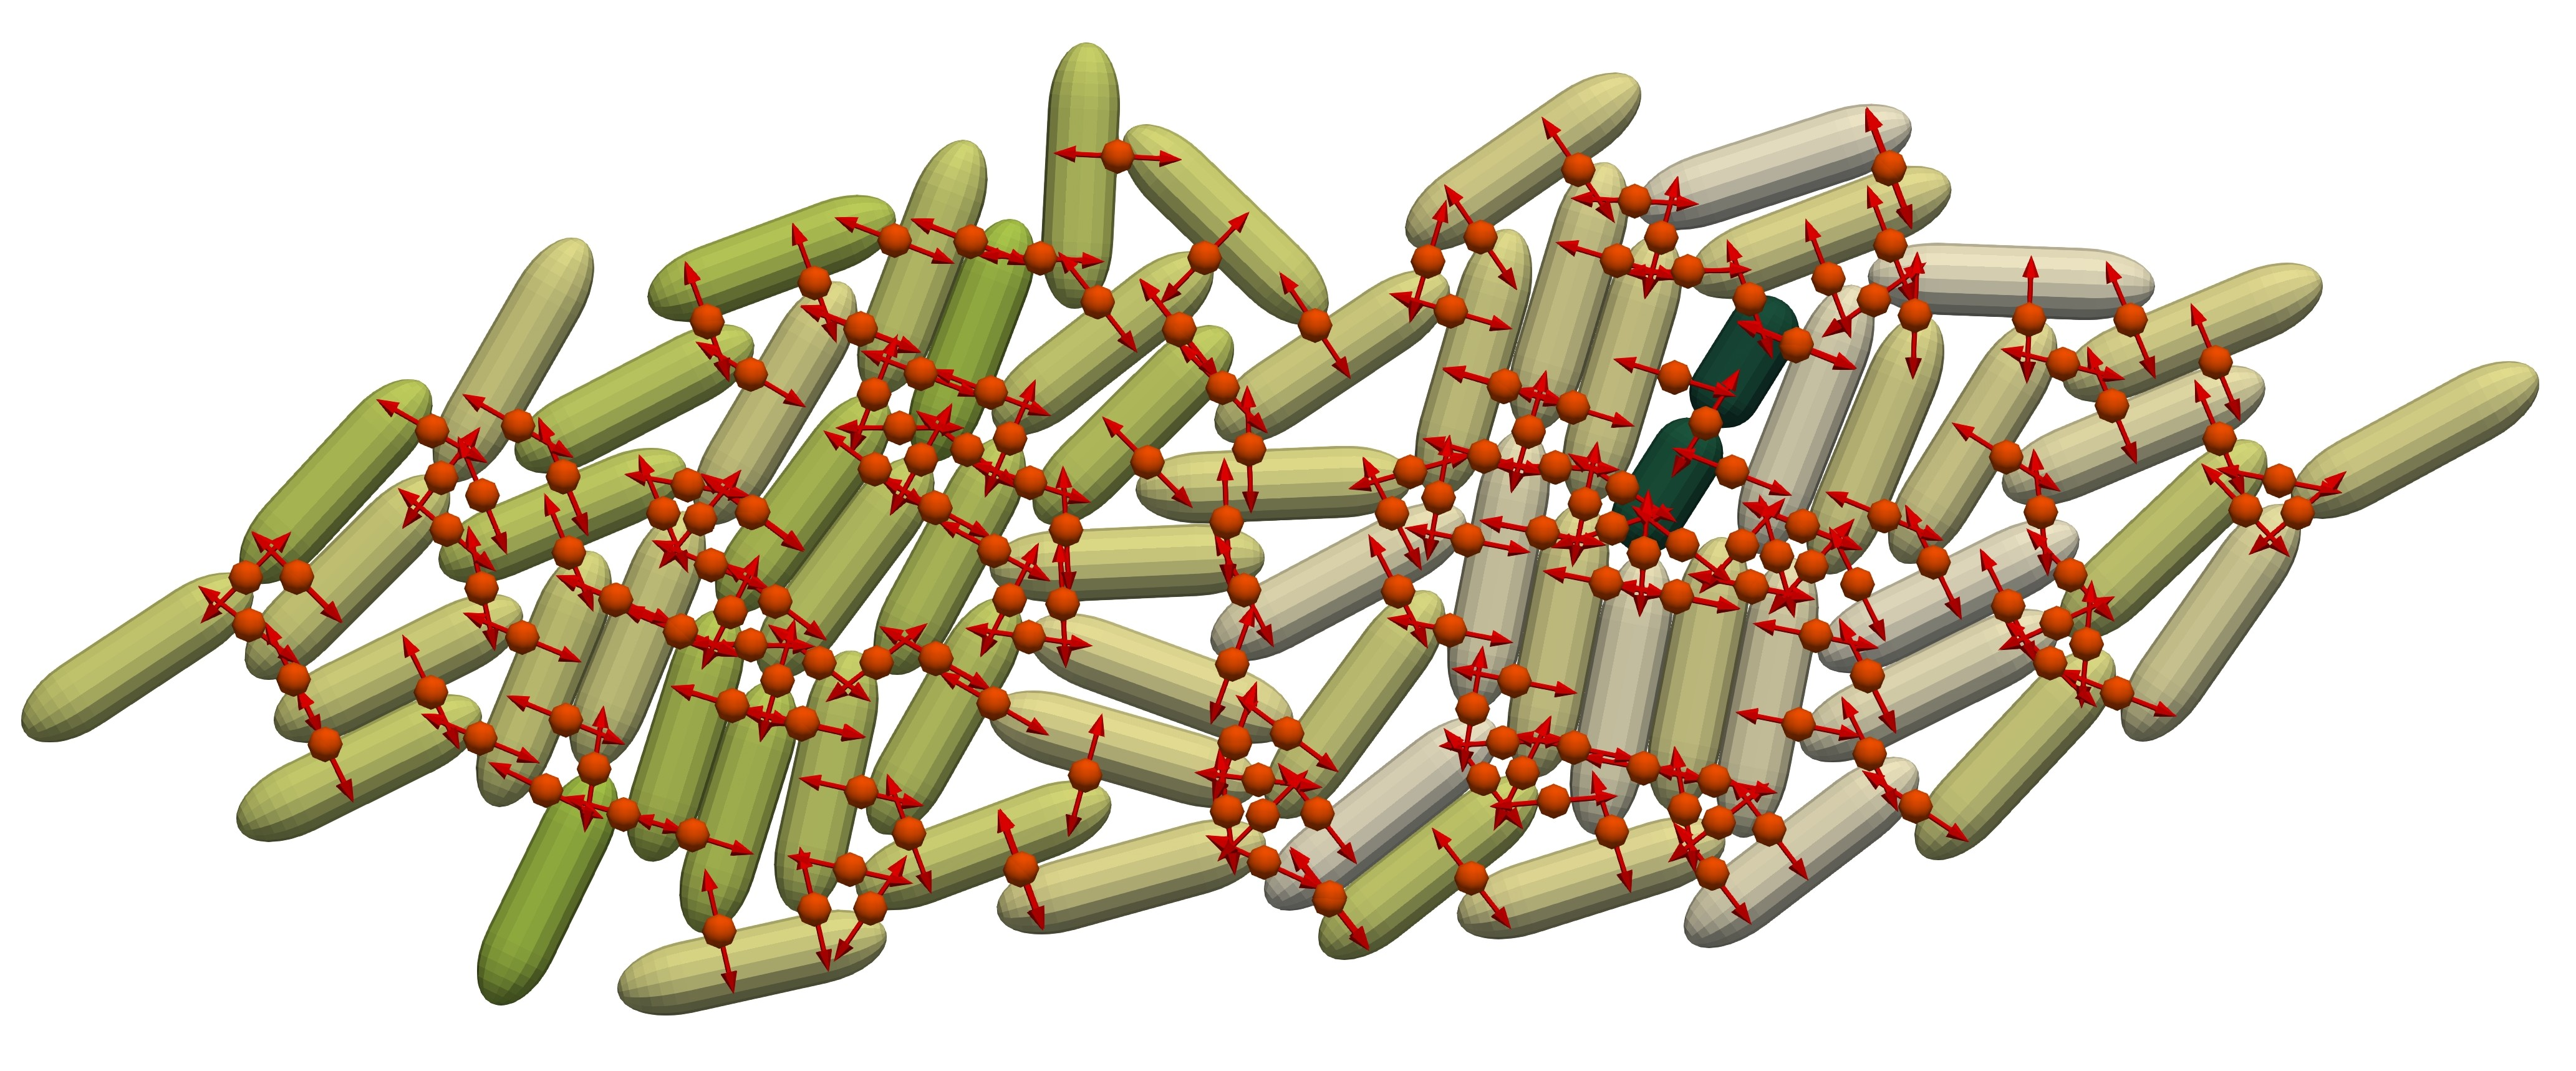
\includegraphics[width=1\textwidth]{figures/constraints.jpeg}
    \end{figure}


    \begin{itemize}
        \item We consider two collision models
        \item Models only differ in how they calculate force magnitudes
    \end{itemize}

\end{frame}


\begin{frame}
    \frametitle{Two Paradigms}

    \vspace{-0.5cm}
    \begin{columns}
        \begin{column}{0.5\textwidth}
            \begin{block}{Soft Model}
                \textbf{Potential-based}

                \begin{itemize}
                    \item Local pairwise forces
                    \item Allows overlap
                    \item Numerically stiff
                    \item Similar to MD simulations
                \end{itemize}

                \begin{equation*}
                    \begin{align}
                                  & \mathbf{F}_{ij} = k \delta^{3/2} \hat{\mathbf{n}} \\
                        \text{  } &
                    \end{align}
                \end{equation*}
                \vfill
            \end{block}
        \end{column}

        \begin{column}{0.5\textwidth}
            \begin{block}{Hard Model \cite{Weady2024}}
                \textbf{Constraint-based}

                \begin{itemize}
                    \item Global optimization problem
                    \item Strict non-overlap
                    \item Single-step solution
                    \item Similar to DEM simulations
                \end{itemize}

                \begin{equation*}
                    \begin{align}
                                     & \mathbf{F}_{ij} = \gamma_{ij} \hat{\mathbf{n}}                              \\
                        \text{s.t. } & \mathbf{0} \leq \boldsymbol{\gamma} \perp \boldsymbol{\Phi} \geq \mathbf{0}
                    \end{align}
                \end{equation*}
                \vfill
            \end{block}
        \end{column}
    \end{columns}

\end{frame}


\begin{frame}
    \frametitle{Soft Model: Hertzian Contact}

    \vspace{0.7cm}

    \begin{columns}[c]
        \begin{column}{0.5\textwidth}
            \begin{equation*}
                \mathbf{F}_{ij} = k_{cc} \sqrt{d} \, \delta^{3/2} \, \hat{\mathbf{n}}
            \end{equation*}

            \vspace{0.3cm}

            \textbf{Characteristics:}
            \begin{itemize}
                \item[$+$] Embarrassingly parallel
                \item[$+$] Simple implementation
                \item[$-$] Numerically stiff
                \item[$-$] Tiny timesteps needed
                \item[$-$] Allows overlap
            \end{itemize}
        \end{column}

        \begin{column}{0.5\textwidth}
            \begin{figure}
                \centering
                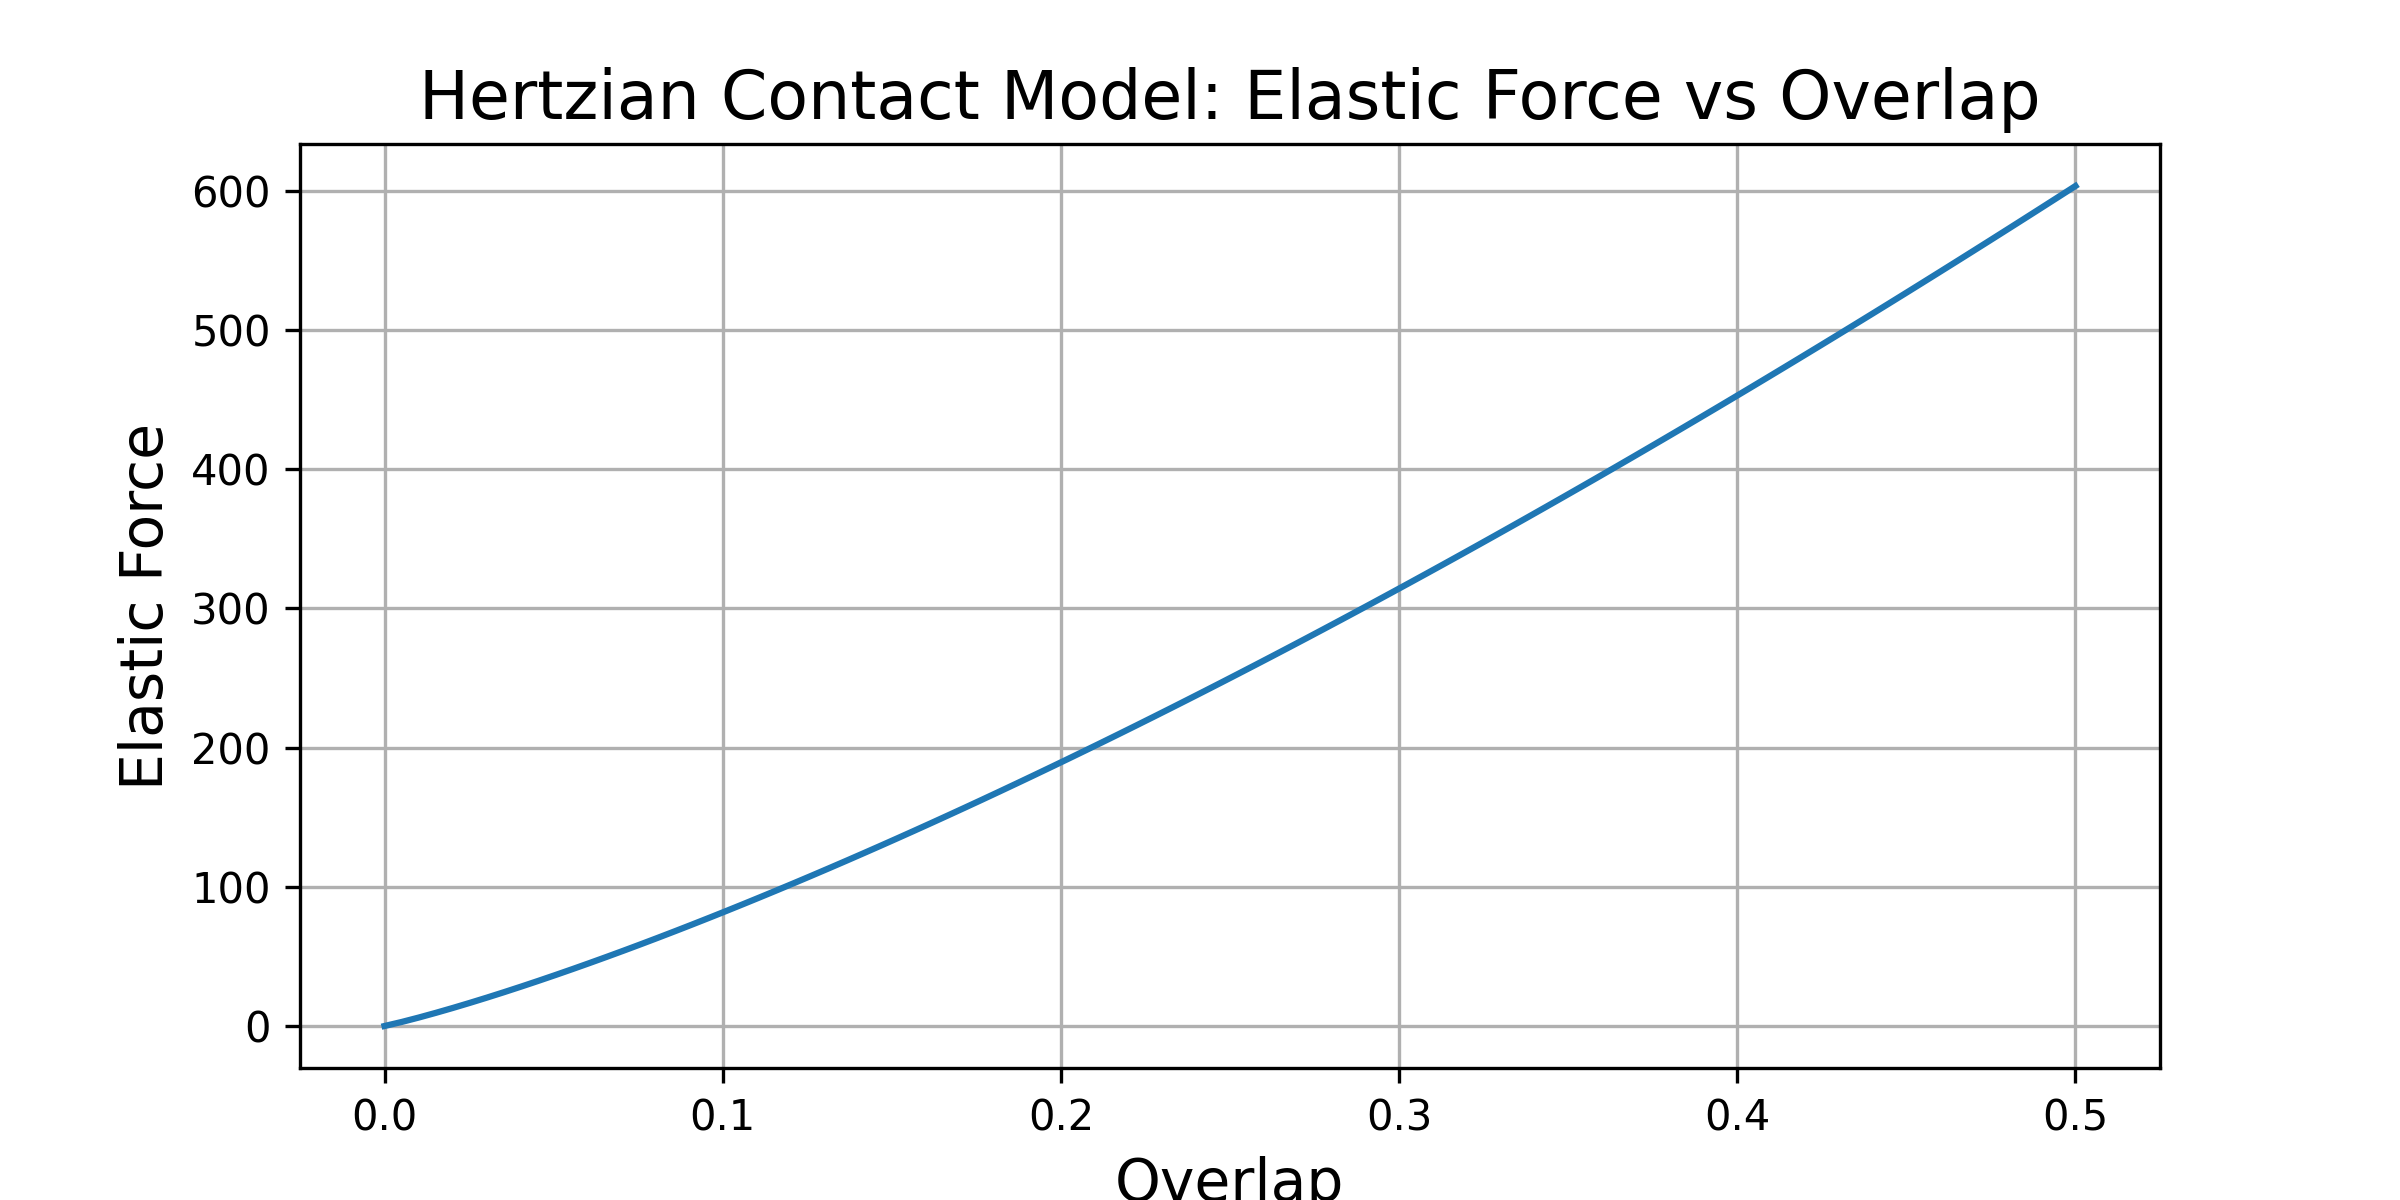
\includegraphics[width=\textwidth]{figures/figures_paper/hertzian_contact_model.png}
                \caption*{\scriptsize{Force increases with overlap}}
            \end{figure}
        \end{column}
    \end{columns}

\end{frame}

\begin{frame}
    \frametitle{Hard Model: Prevent overlap via optimization}

    \begin{itemize}
        \item Define signed distance between cells:
              \[
                  \boldsymbol{\Phi}_{ij} =
                  \begin{cases}
                      > 0 & \text{no contact} \\
                      = 0 & \text{contact}    \\
                      < 0 & \text{overlap}
                  \end{cases}
              \]

        \item Find contact forces $\boldsymbol{\gamma}$ s.t.
              \[
                  \boldsymbol{0} \le \boldsymbol{\gamma} \perp \boldsymbol{\Phi}^{k+1} \ge \boldsymbol{0}
              \]

        \item Approximate how individual forces $\boldsymbol{\gamma}_{i}$ affect $\boldsymbol{\Phi}^{k+1}$
        \item Solve convex optimization problem:
              \[
                  \min_{\boldsymbol{\gamma} \ge 0} E(\boldsymbol{\gamma})
                  = \boldsymbol{\gamma}^\top \boldsymbol{\Phi}^k
                  + \tfrac{\Delta t}{2}\boldsymbol{\gamma}^\top
                  \mathbfcal{D}^\top \mathbfcal{M}^k \mathbfcal{D}\boldsymbol{\gamma}
                  + \mathbf{1}^\top \tfrac{\Delta t}{\lambda}
                  \left( \tfrac{\boldsymbol{\ell}}{\tau} \odot
                  e^{-\lambda \mathbfcal{L} \boldsymbol{\gamma}} \right)
              \]

    \end{itemize}

\end{frame}

\begin{frame}
    \frametitle{Example: Hard Model}

    \vspace{-0.5cm}
    \begin{columns}[c]
        \begin{column}{0.4\textwidth}
            \begin{figure}
                \centering
                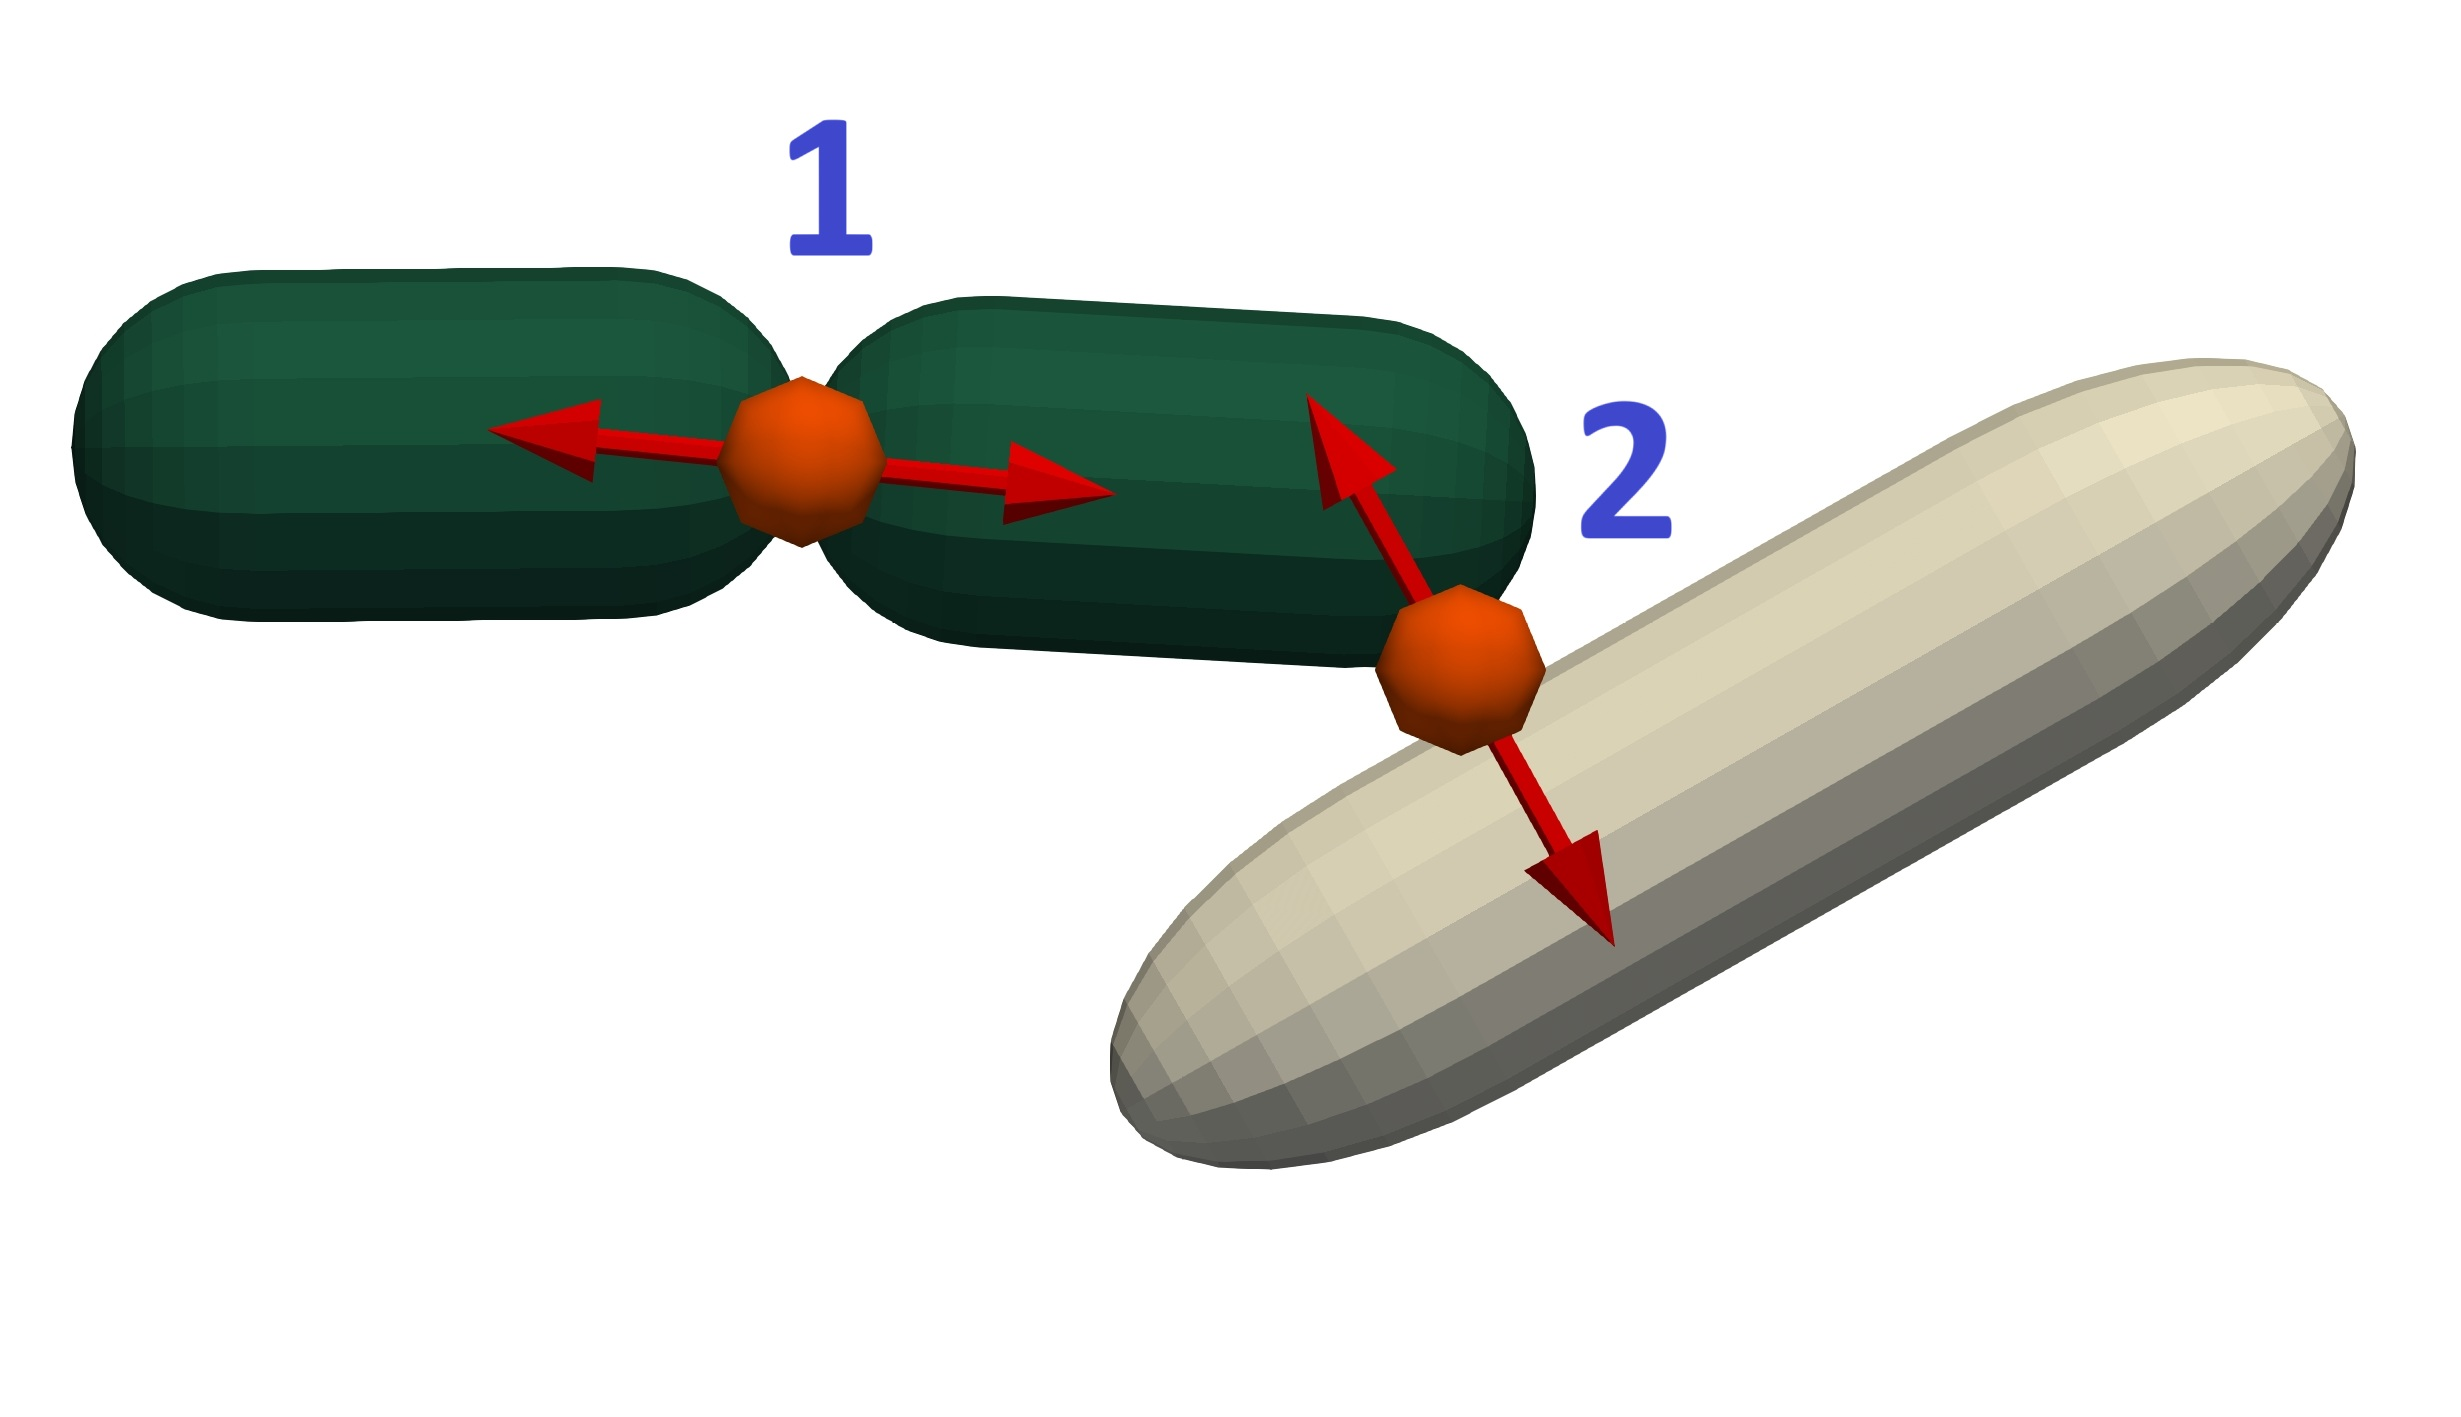
\includegraphics[width=1\textwidth]{figures/constraints_example_small.jpeg}
            \end{figure}
        \end{column}

        \begin{column}{0.65\textwidth}
            \begin{figure}
                \centering
                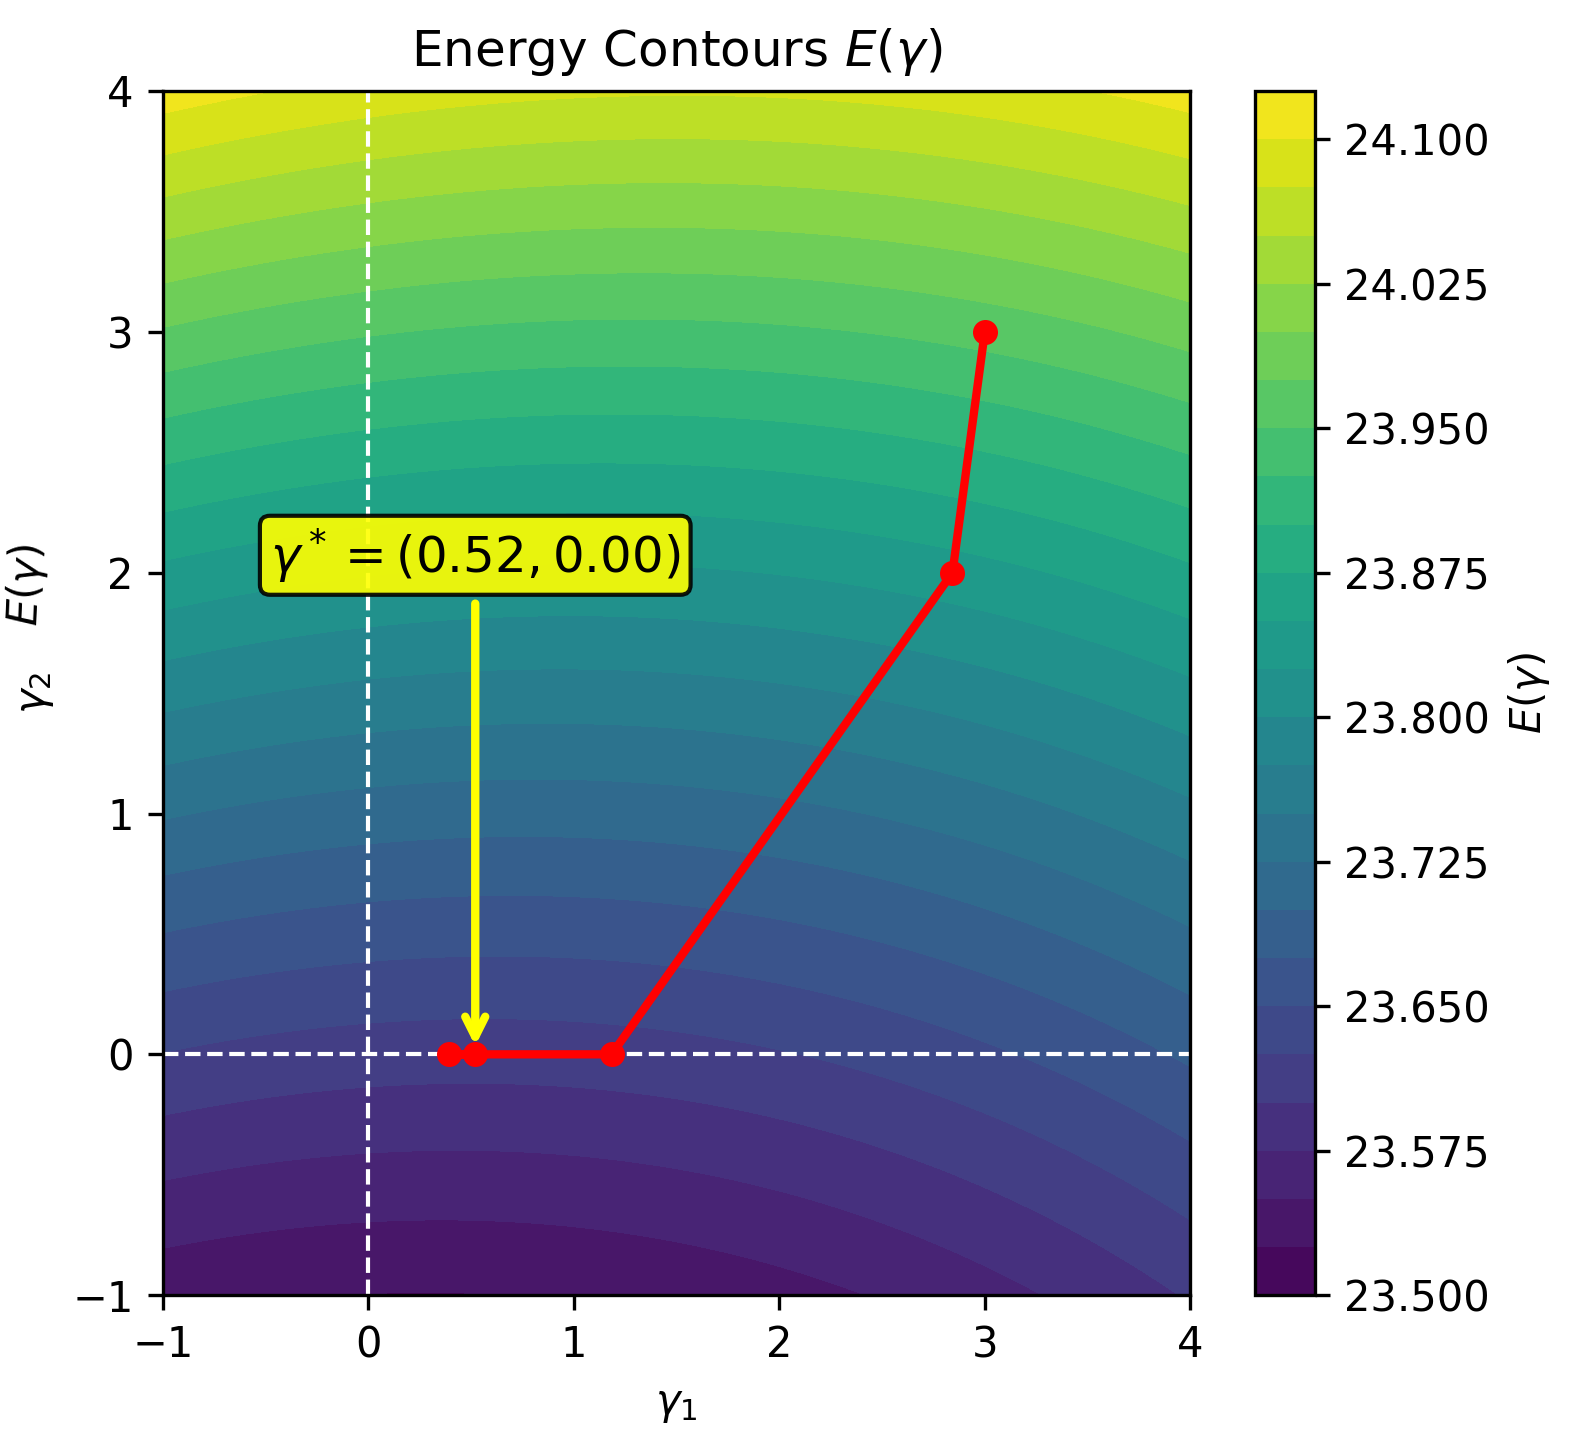
\includegraphics[width=1\textwidth]{figures/energy_surface_contours.png}
            \end{figure}
        \end{column}
    \end{columns}

\end{frame}

\begin{frame}
    \frametitle{Hard Model: Performance}

    \vspace{0.8cm}

    \begin{columns}[c]
        \begin{column}{0.45\textwidth}
            \textbf{Characteristics:}
            \begin{itemize}
                \item[$+$] Less numerical stiffness
                \item[$+$] Larger timesteps possible
                \item[$+$] Strict non-overlap
                \item[$-$] High per-step cost
                \item[$-$] Complex implementation
                \item[$-$] Requires multiple passes
            \end{itemize}
        \end{column}

        \begin{column}{0.6\textwidth}
            \begin{figure}
                \centering
                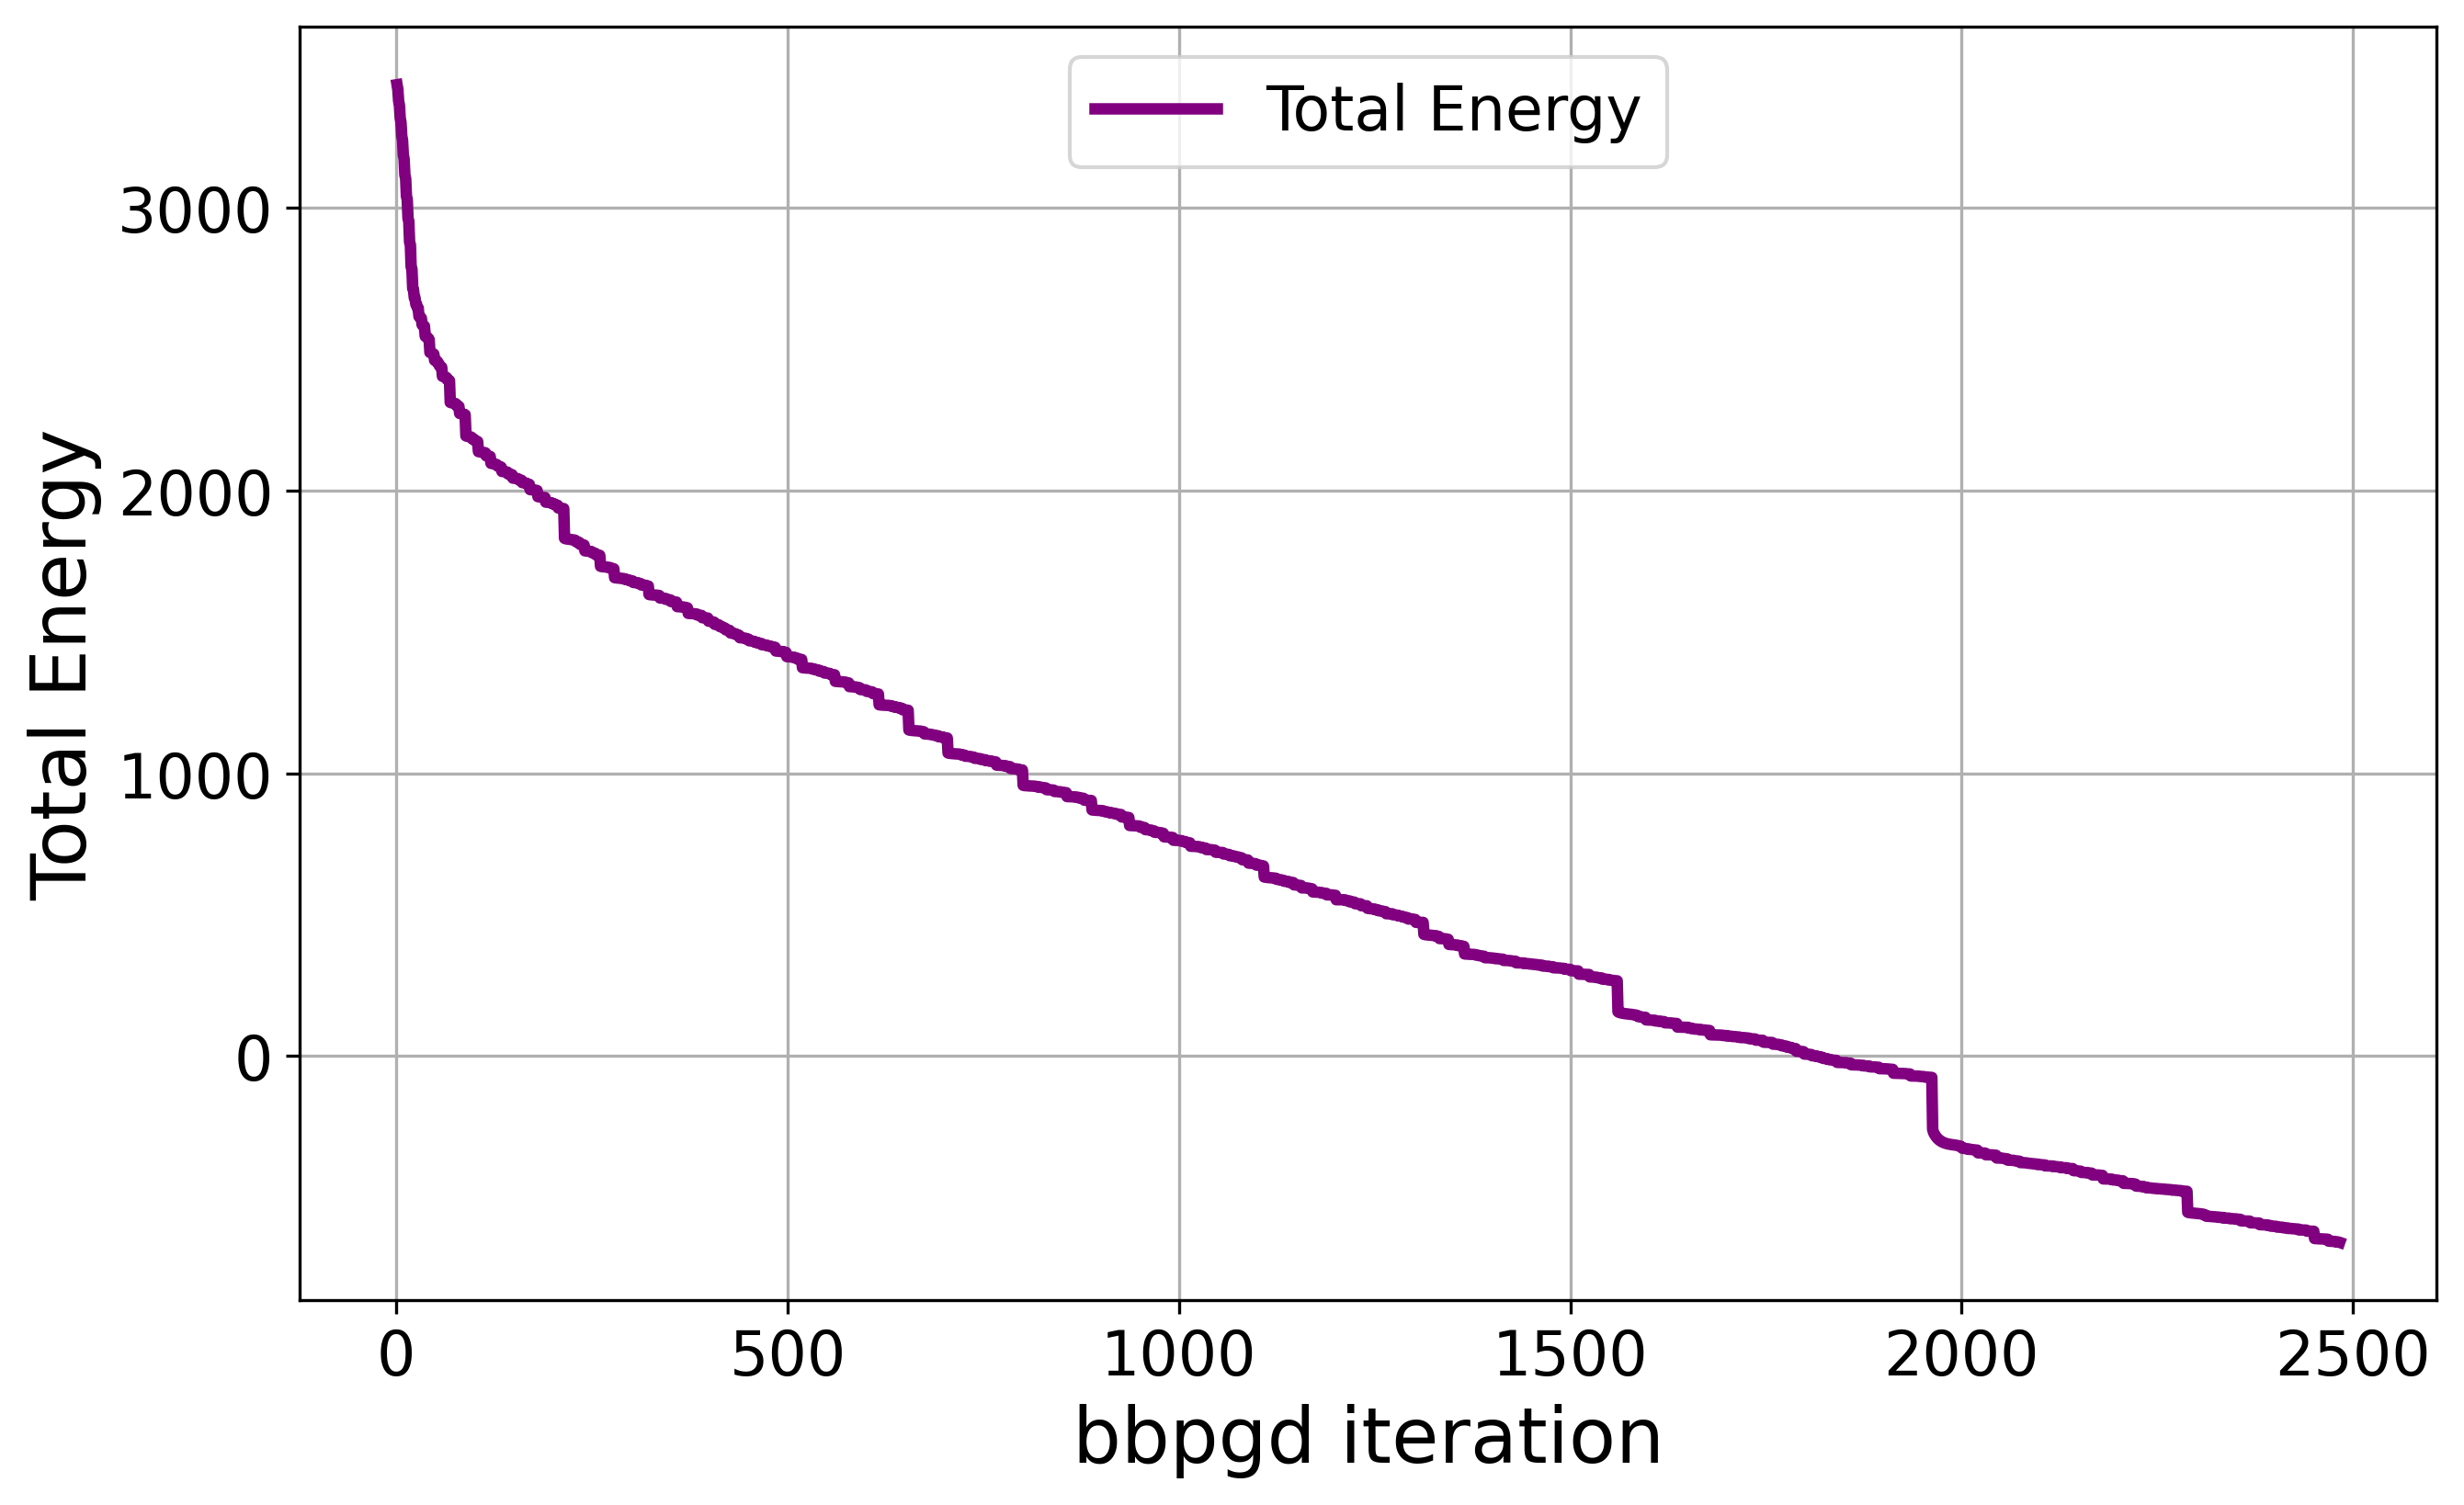
\includegraphics[width=\textwidth]{figures/figures_paper/bbpgd/bbpgd_total_energy.png}
            \end{figure}
        \end{column}
    \end{columns}

\end{frame}

% ============================================================
% SECTION 5: BIOLOGICAL VALIDATION
% ============================================================

\section{Pattern Formation Results}

\begin{frame}
    \frametitle{Concentric Ring Formation}

    \begin{columns}[c]
        \begin{column}{0.48\textwidth}
            \centering
            \textbf{Hard Model}\\[0.3em]
            {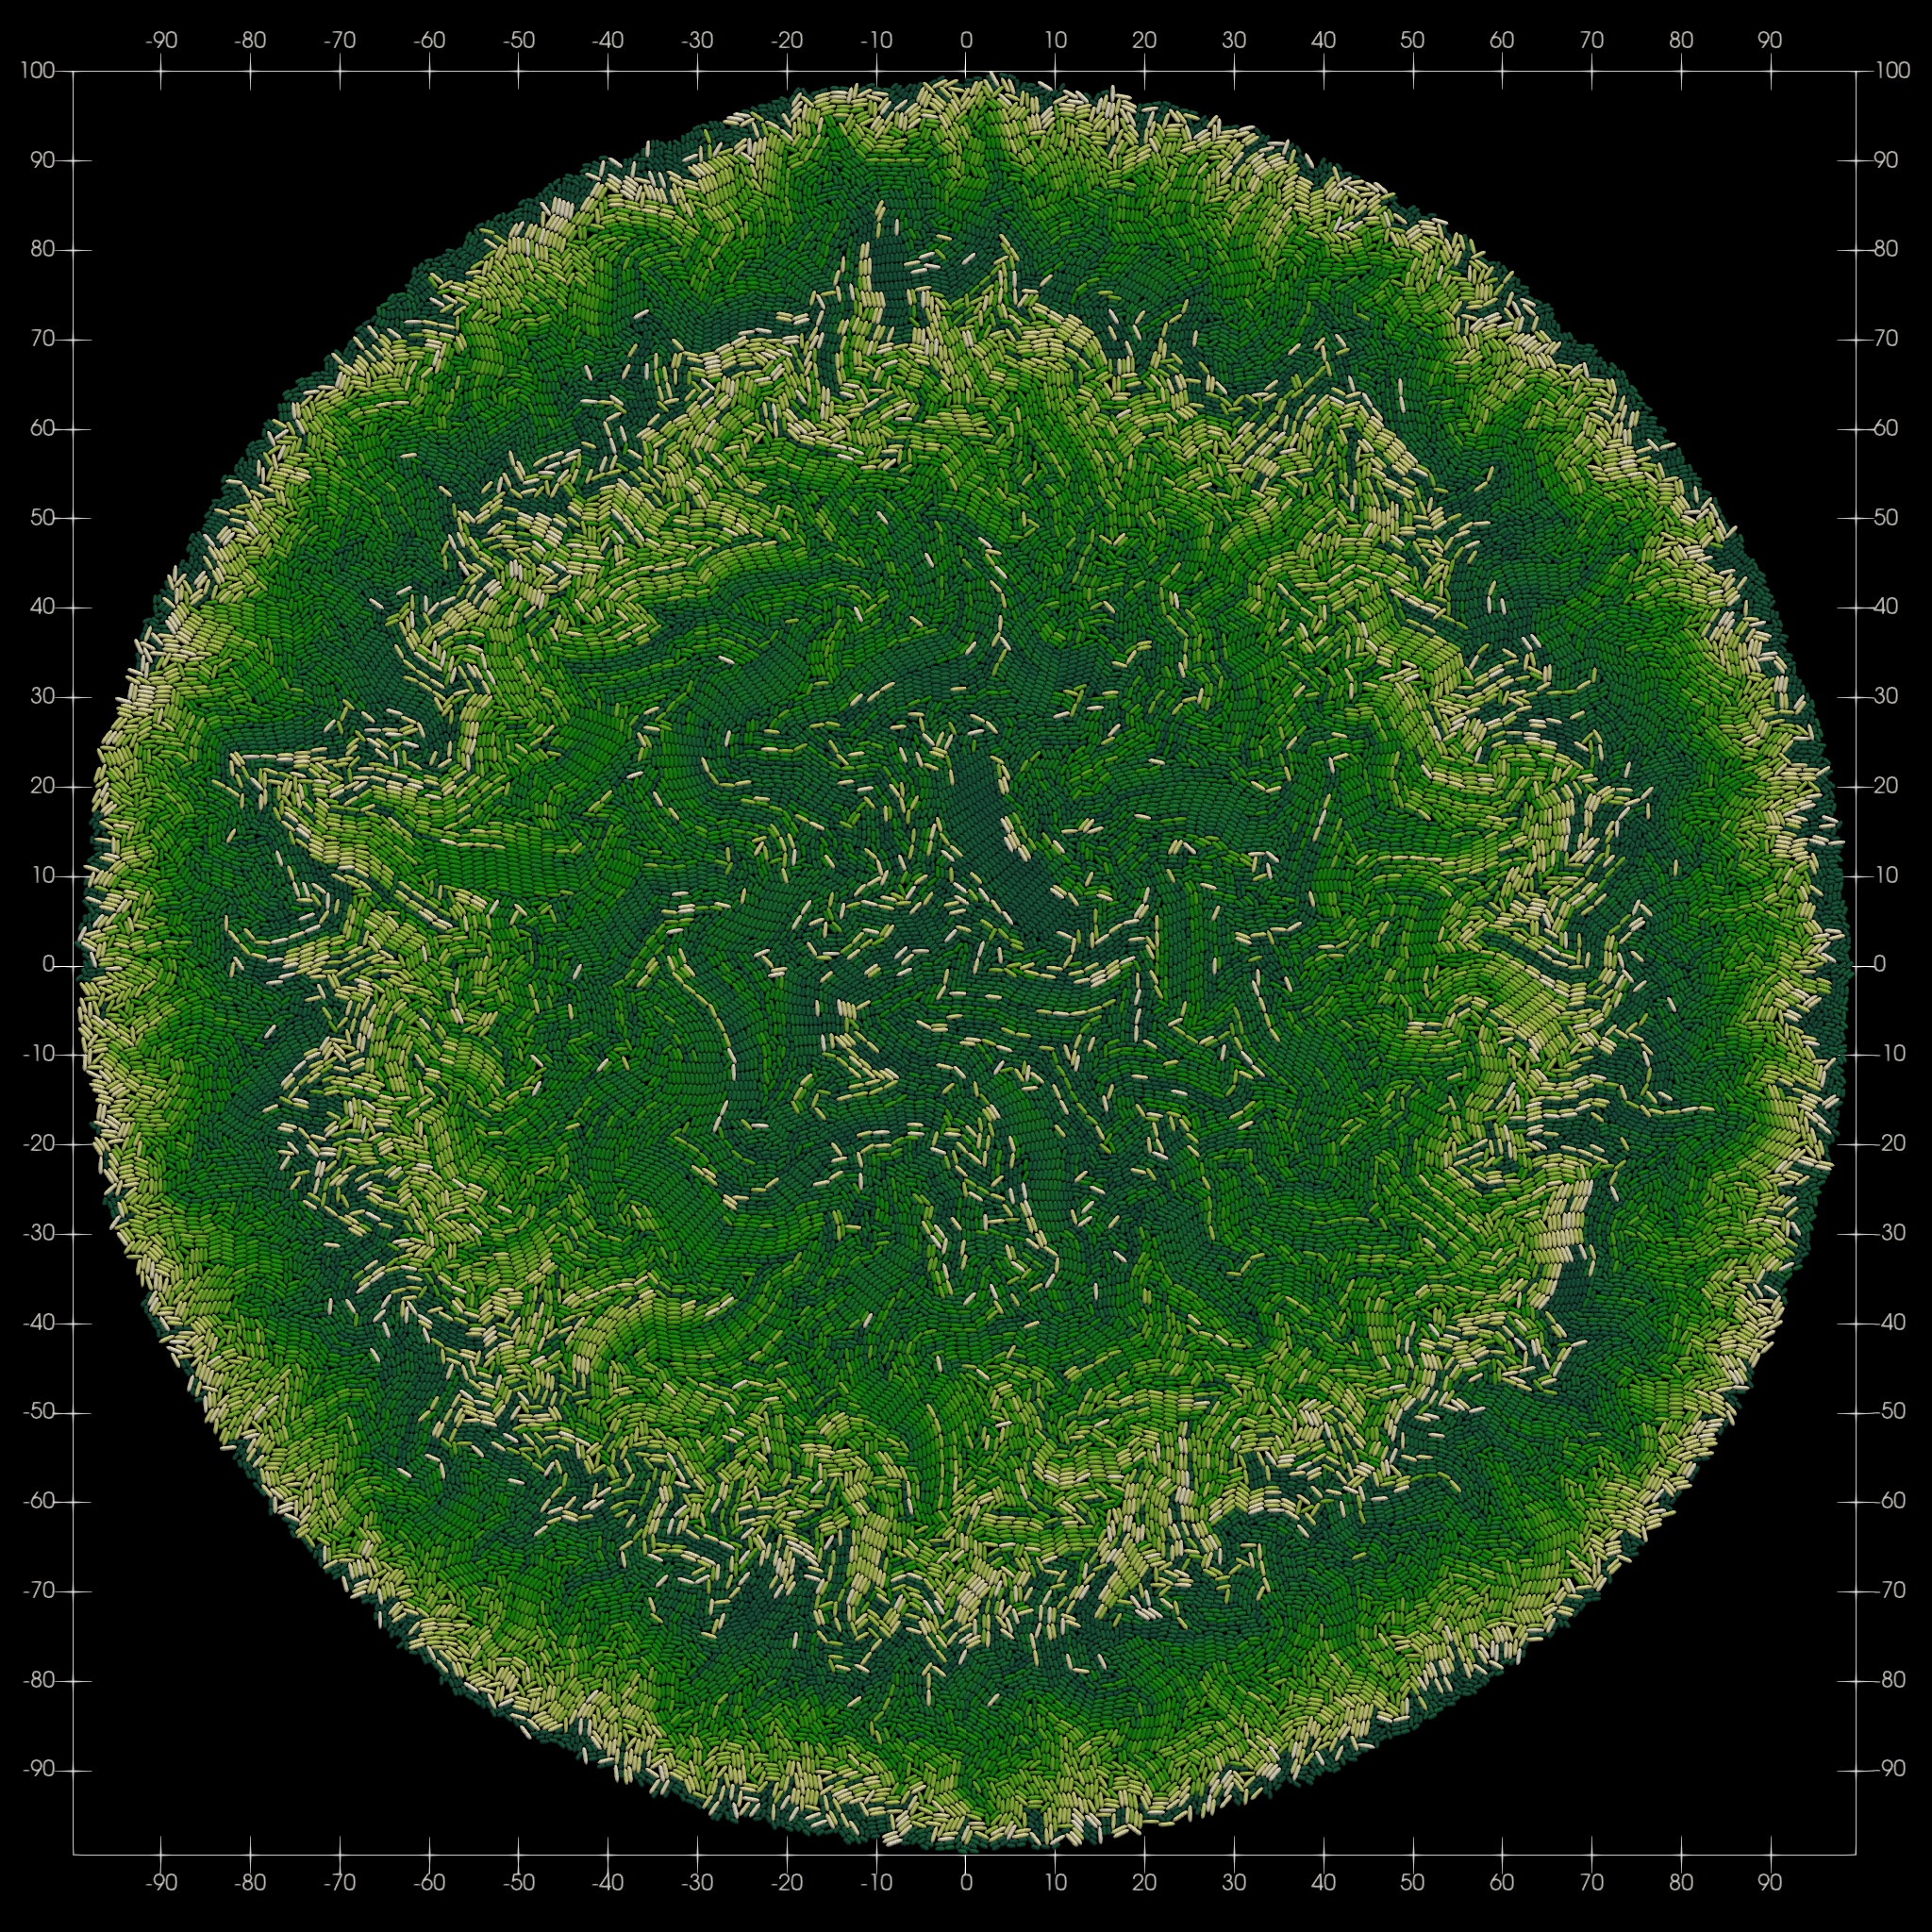
\includegraphics[width=\textwidth]{figures/figures_paper/growth/hard_e-3/hard_e-3.0198.jpeg}}\\[0.6em]
            \small
            \href{https://home.cit.tum.de/~ler/bacteria/videos/hard_e-3.mp4}{\textcolor{blue}{{View video}}}
        \end{column}

        \begin{column}{0.48\textwidth}
            \centering
            \textbf{Soft Model}\\[0.3em]
            {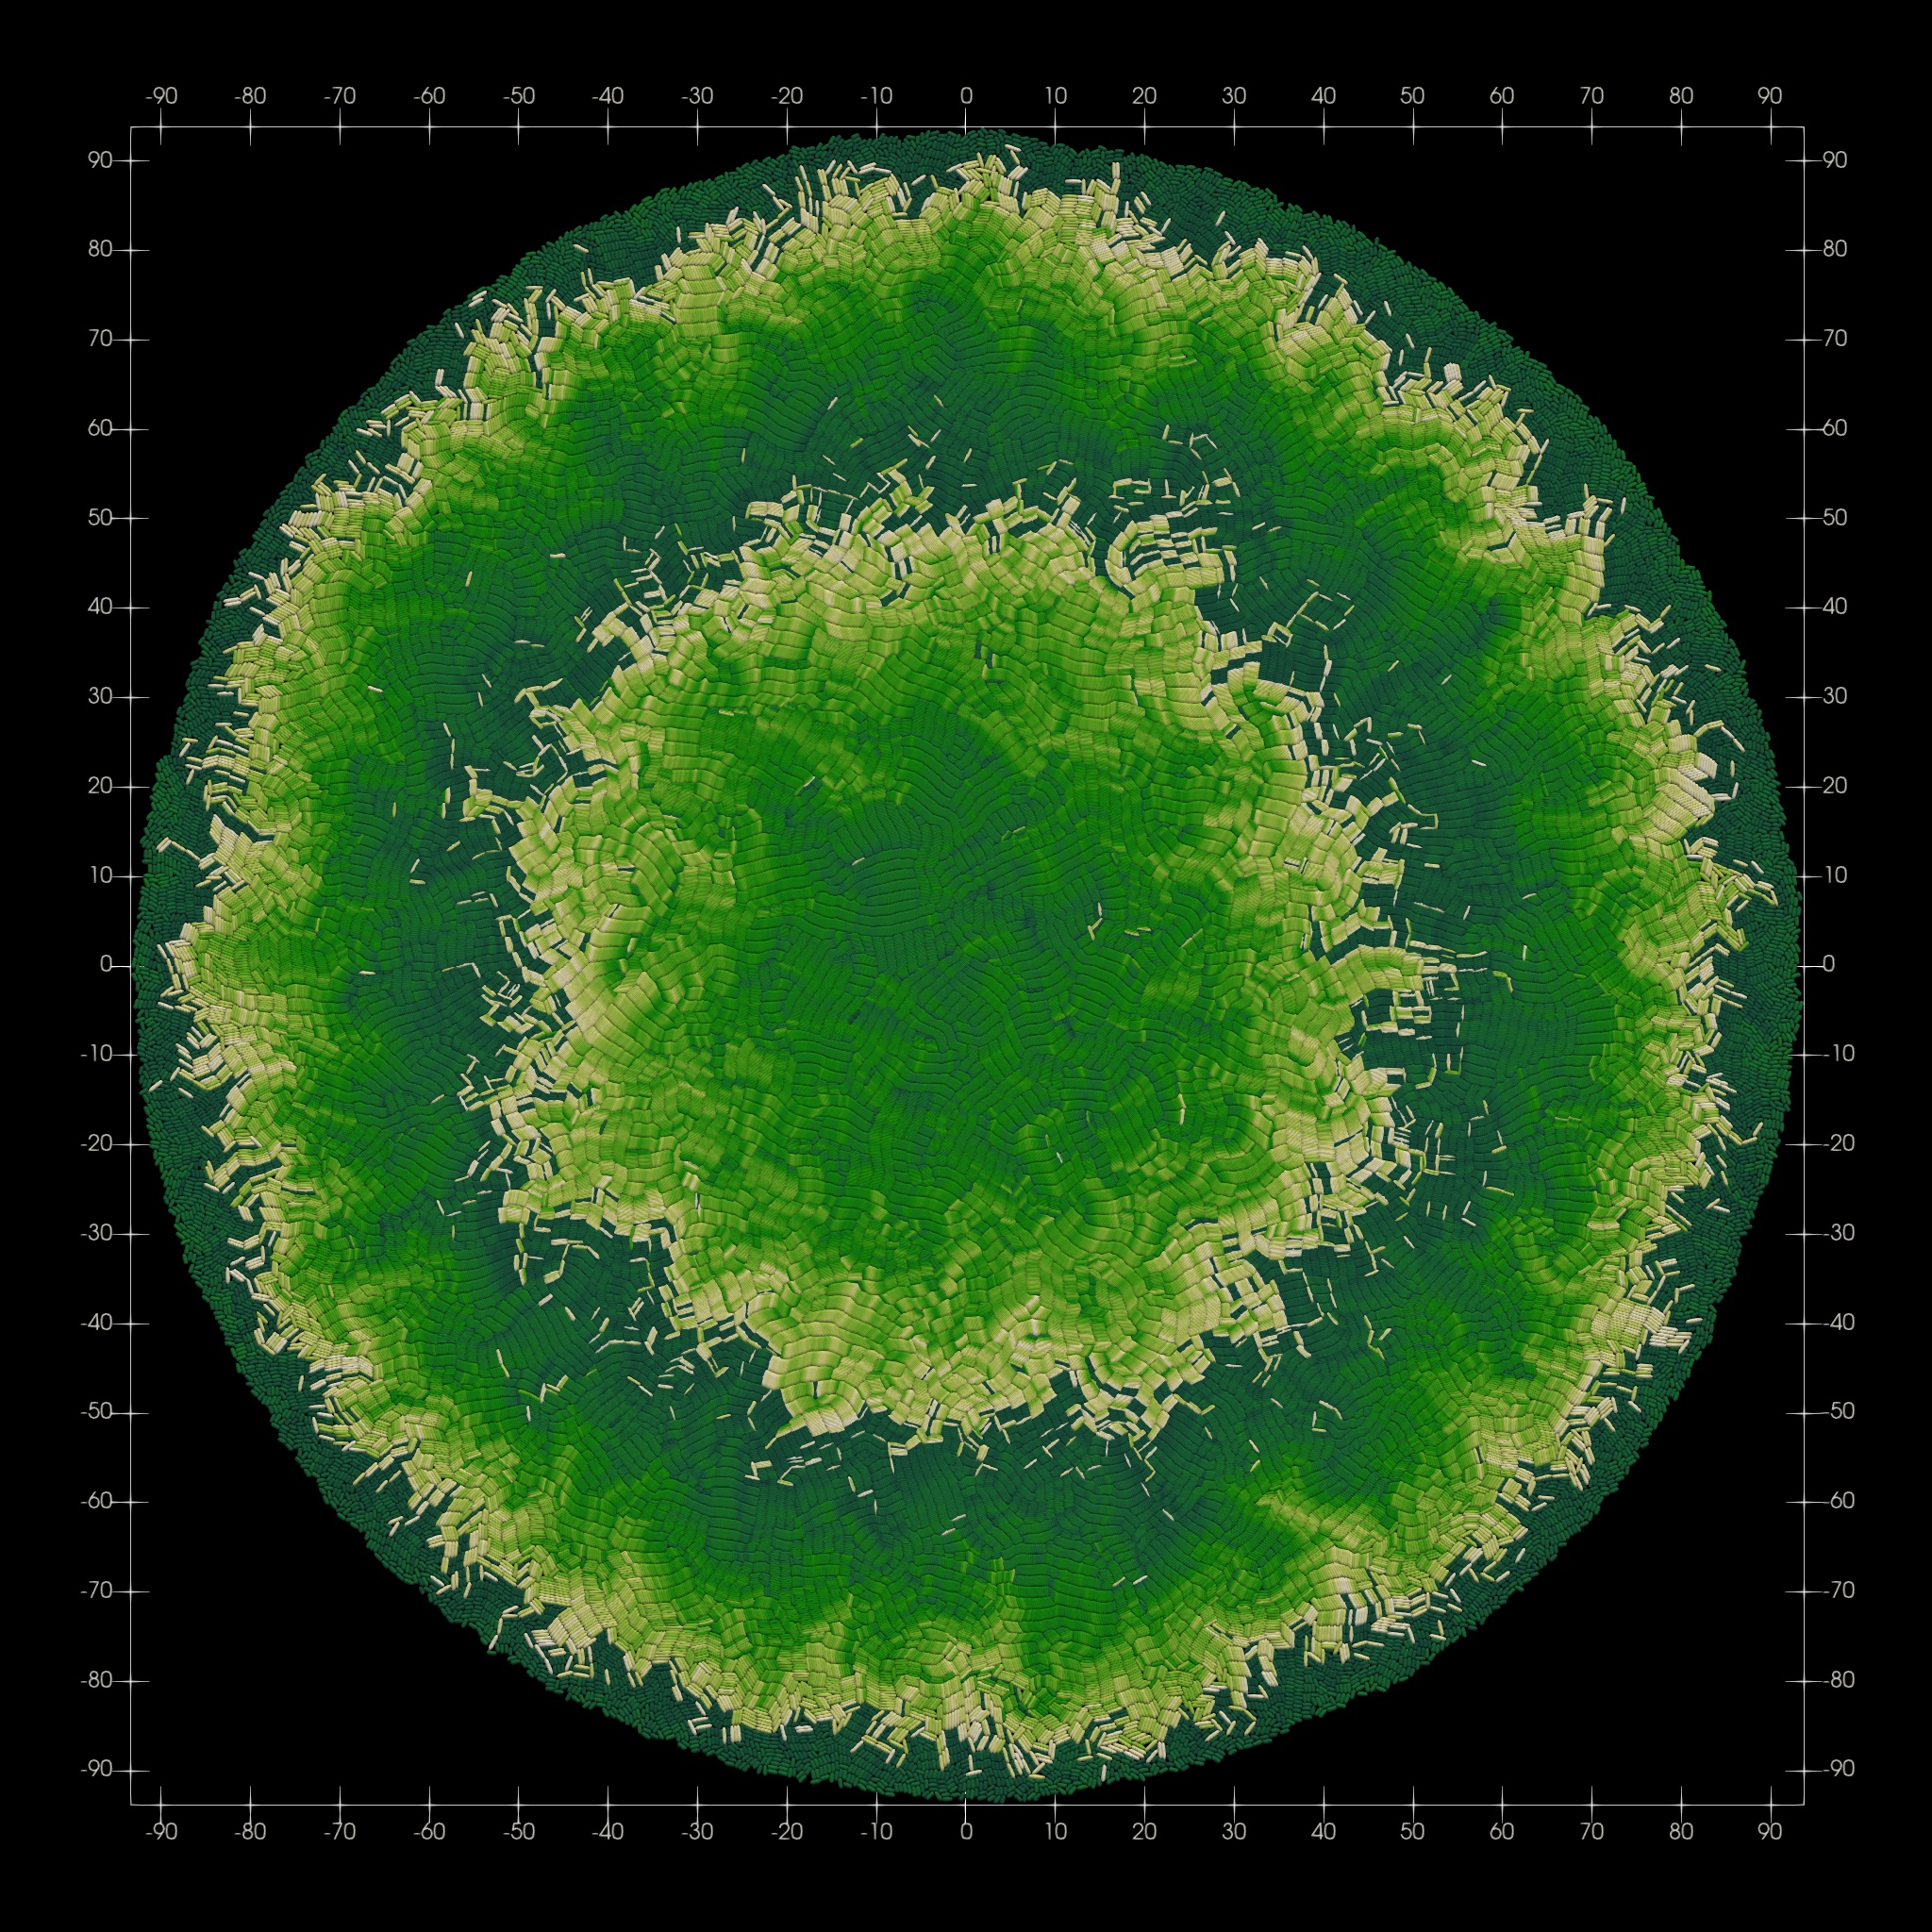
\includegraphics[width=\textwidth]{figures/figures_paper/growth/soft_e-3/soft_e-3.0187.jpeg}}\\[0.6em]
            \small
            \href{https://home.cit.tum.de/~ler/bacteria/videos/soft_e-3.mp4}{\textcolor{blue}{{View video}}}
        \end{column}
    \end{columns}
\end{frame}

% \begin{frame}
%     \frametitle{Ring Formation Across Parameters}

%     \vspace{-0.3cm}
%     \begin{figure}
%         \centering
%         \begin{tabular}{r M{0.25\textwidth} M{0.25\textwidth} M{0.25\textwidth}}
%                                                                                                              & $\lambda = 10^{-4}$        & $\lambda = 10^{-3}$      & $\lambda = 10^{-2}$
%             \\[3pt]
%             \textbf{Hard}                                                                                    &
%             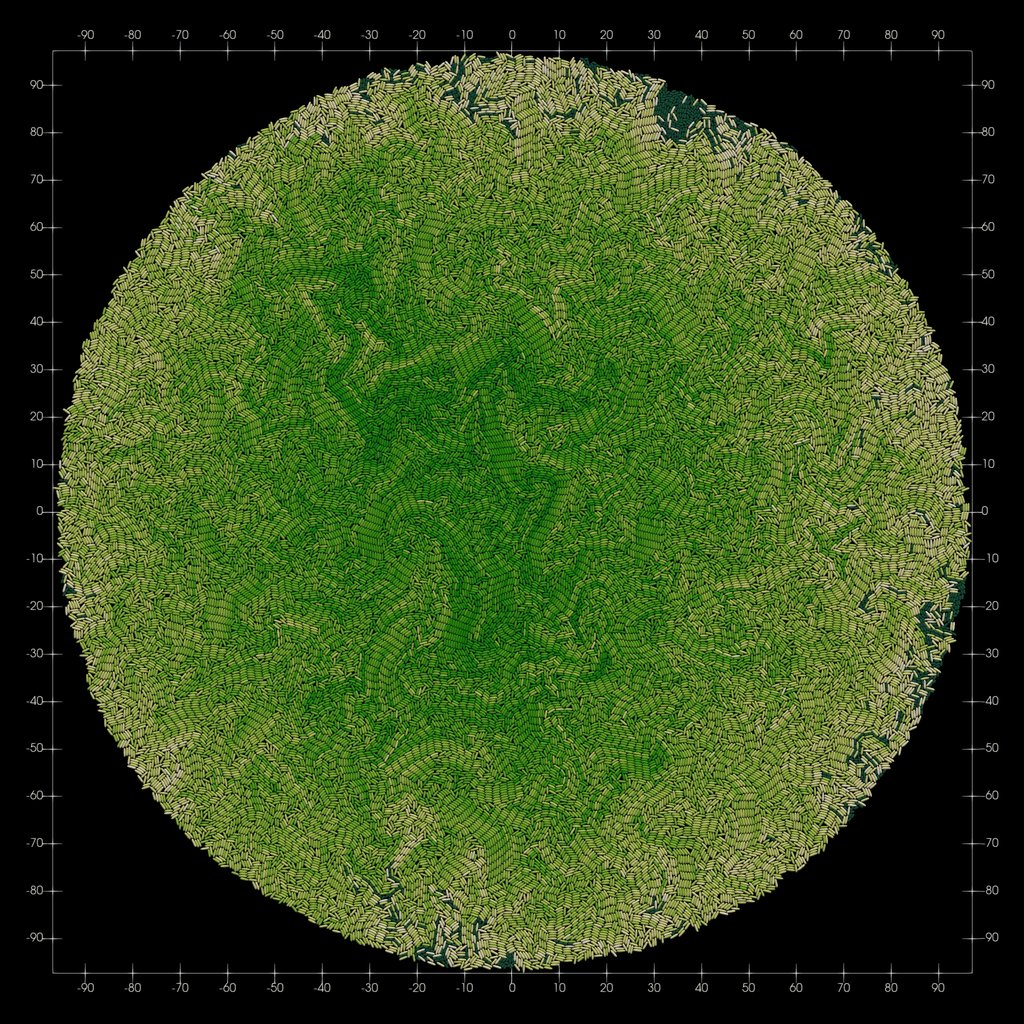
\includegraphics[width=0.25\textwidth]{figures/figures_paper/growth/hard_e-4/hard_e-4.0192.jpeg} &
%             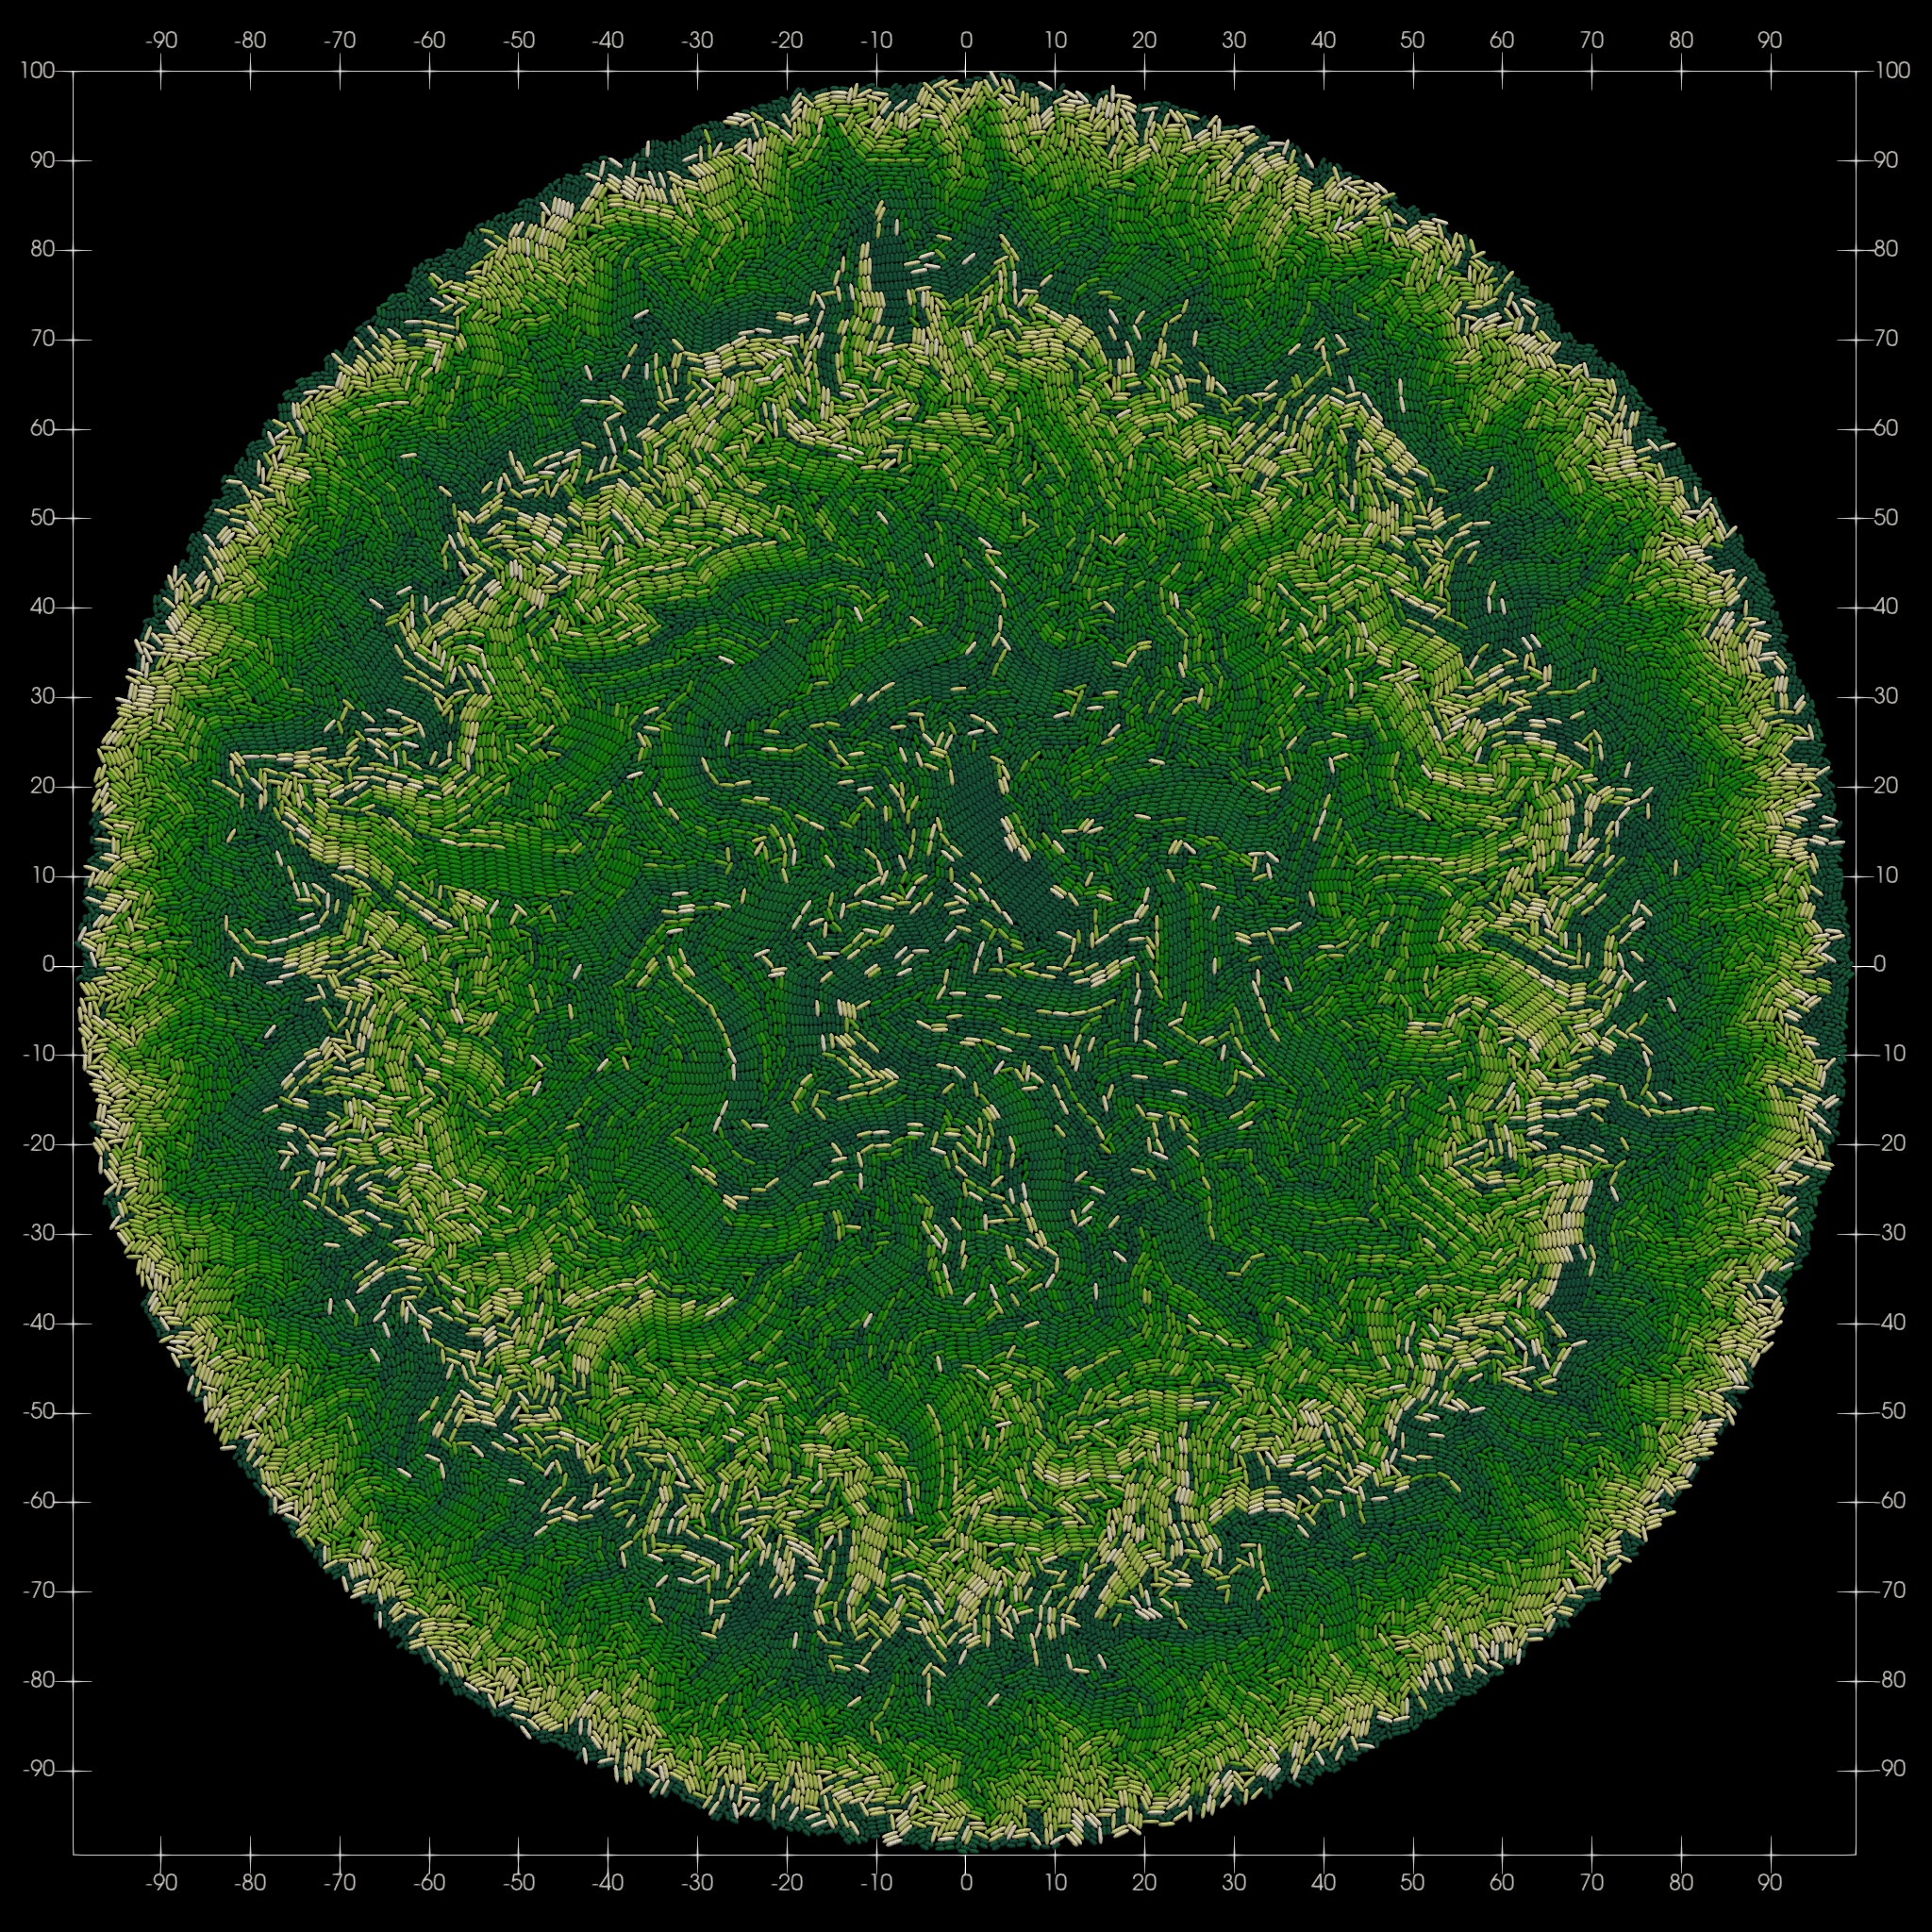
\includegraphics[width=0.25\textwidth]{figures/figures_paper/growth/hard_e-3/hard_e-3.0198.jpeg} &
%             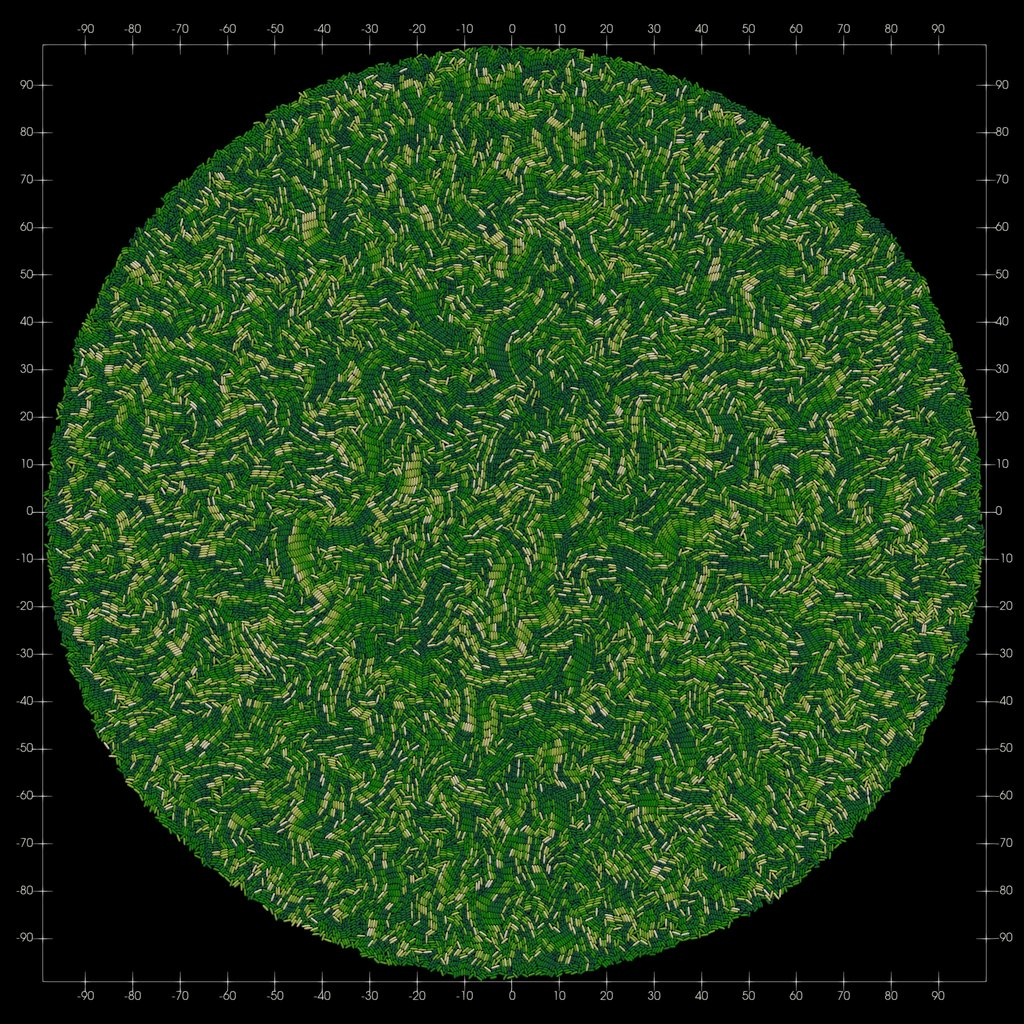
\includegraphics[width=0.25\textwidth]{figures/figures_paper/growth/hard_e-2/hard_e-2.0199.jpeg}                                                                                          \\[3pt]

%             \textbf{Soft}                                                                                    &
%             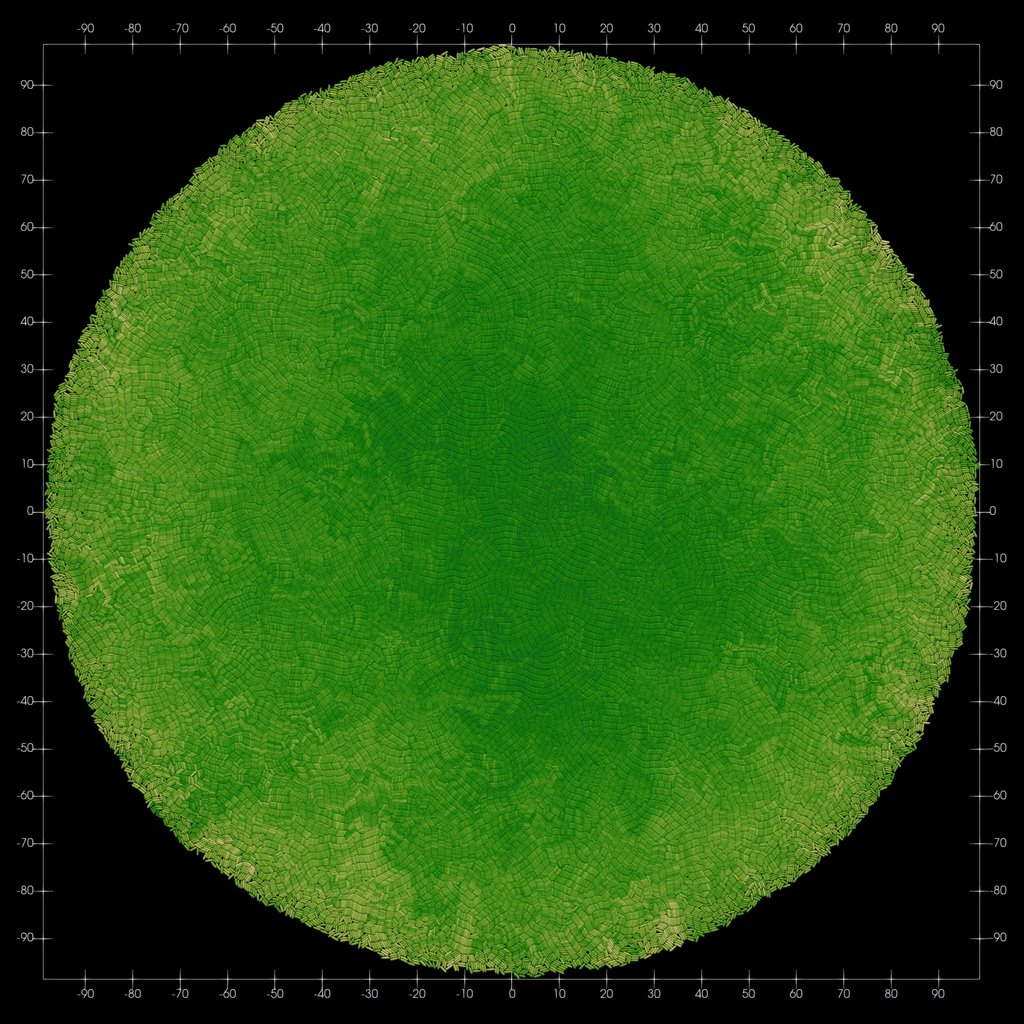
\includegraphics[width=0.25\textwidth]{figures/figures_paper/growth/soft_e-4/soft_e-4.0198.jpeg} &
%             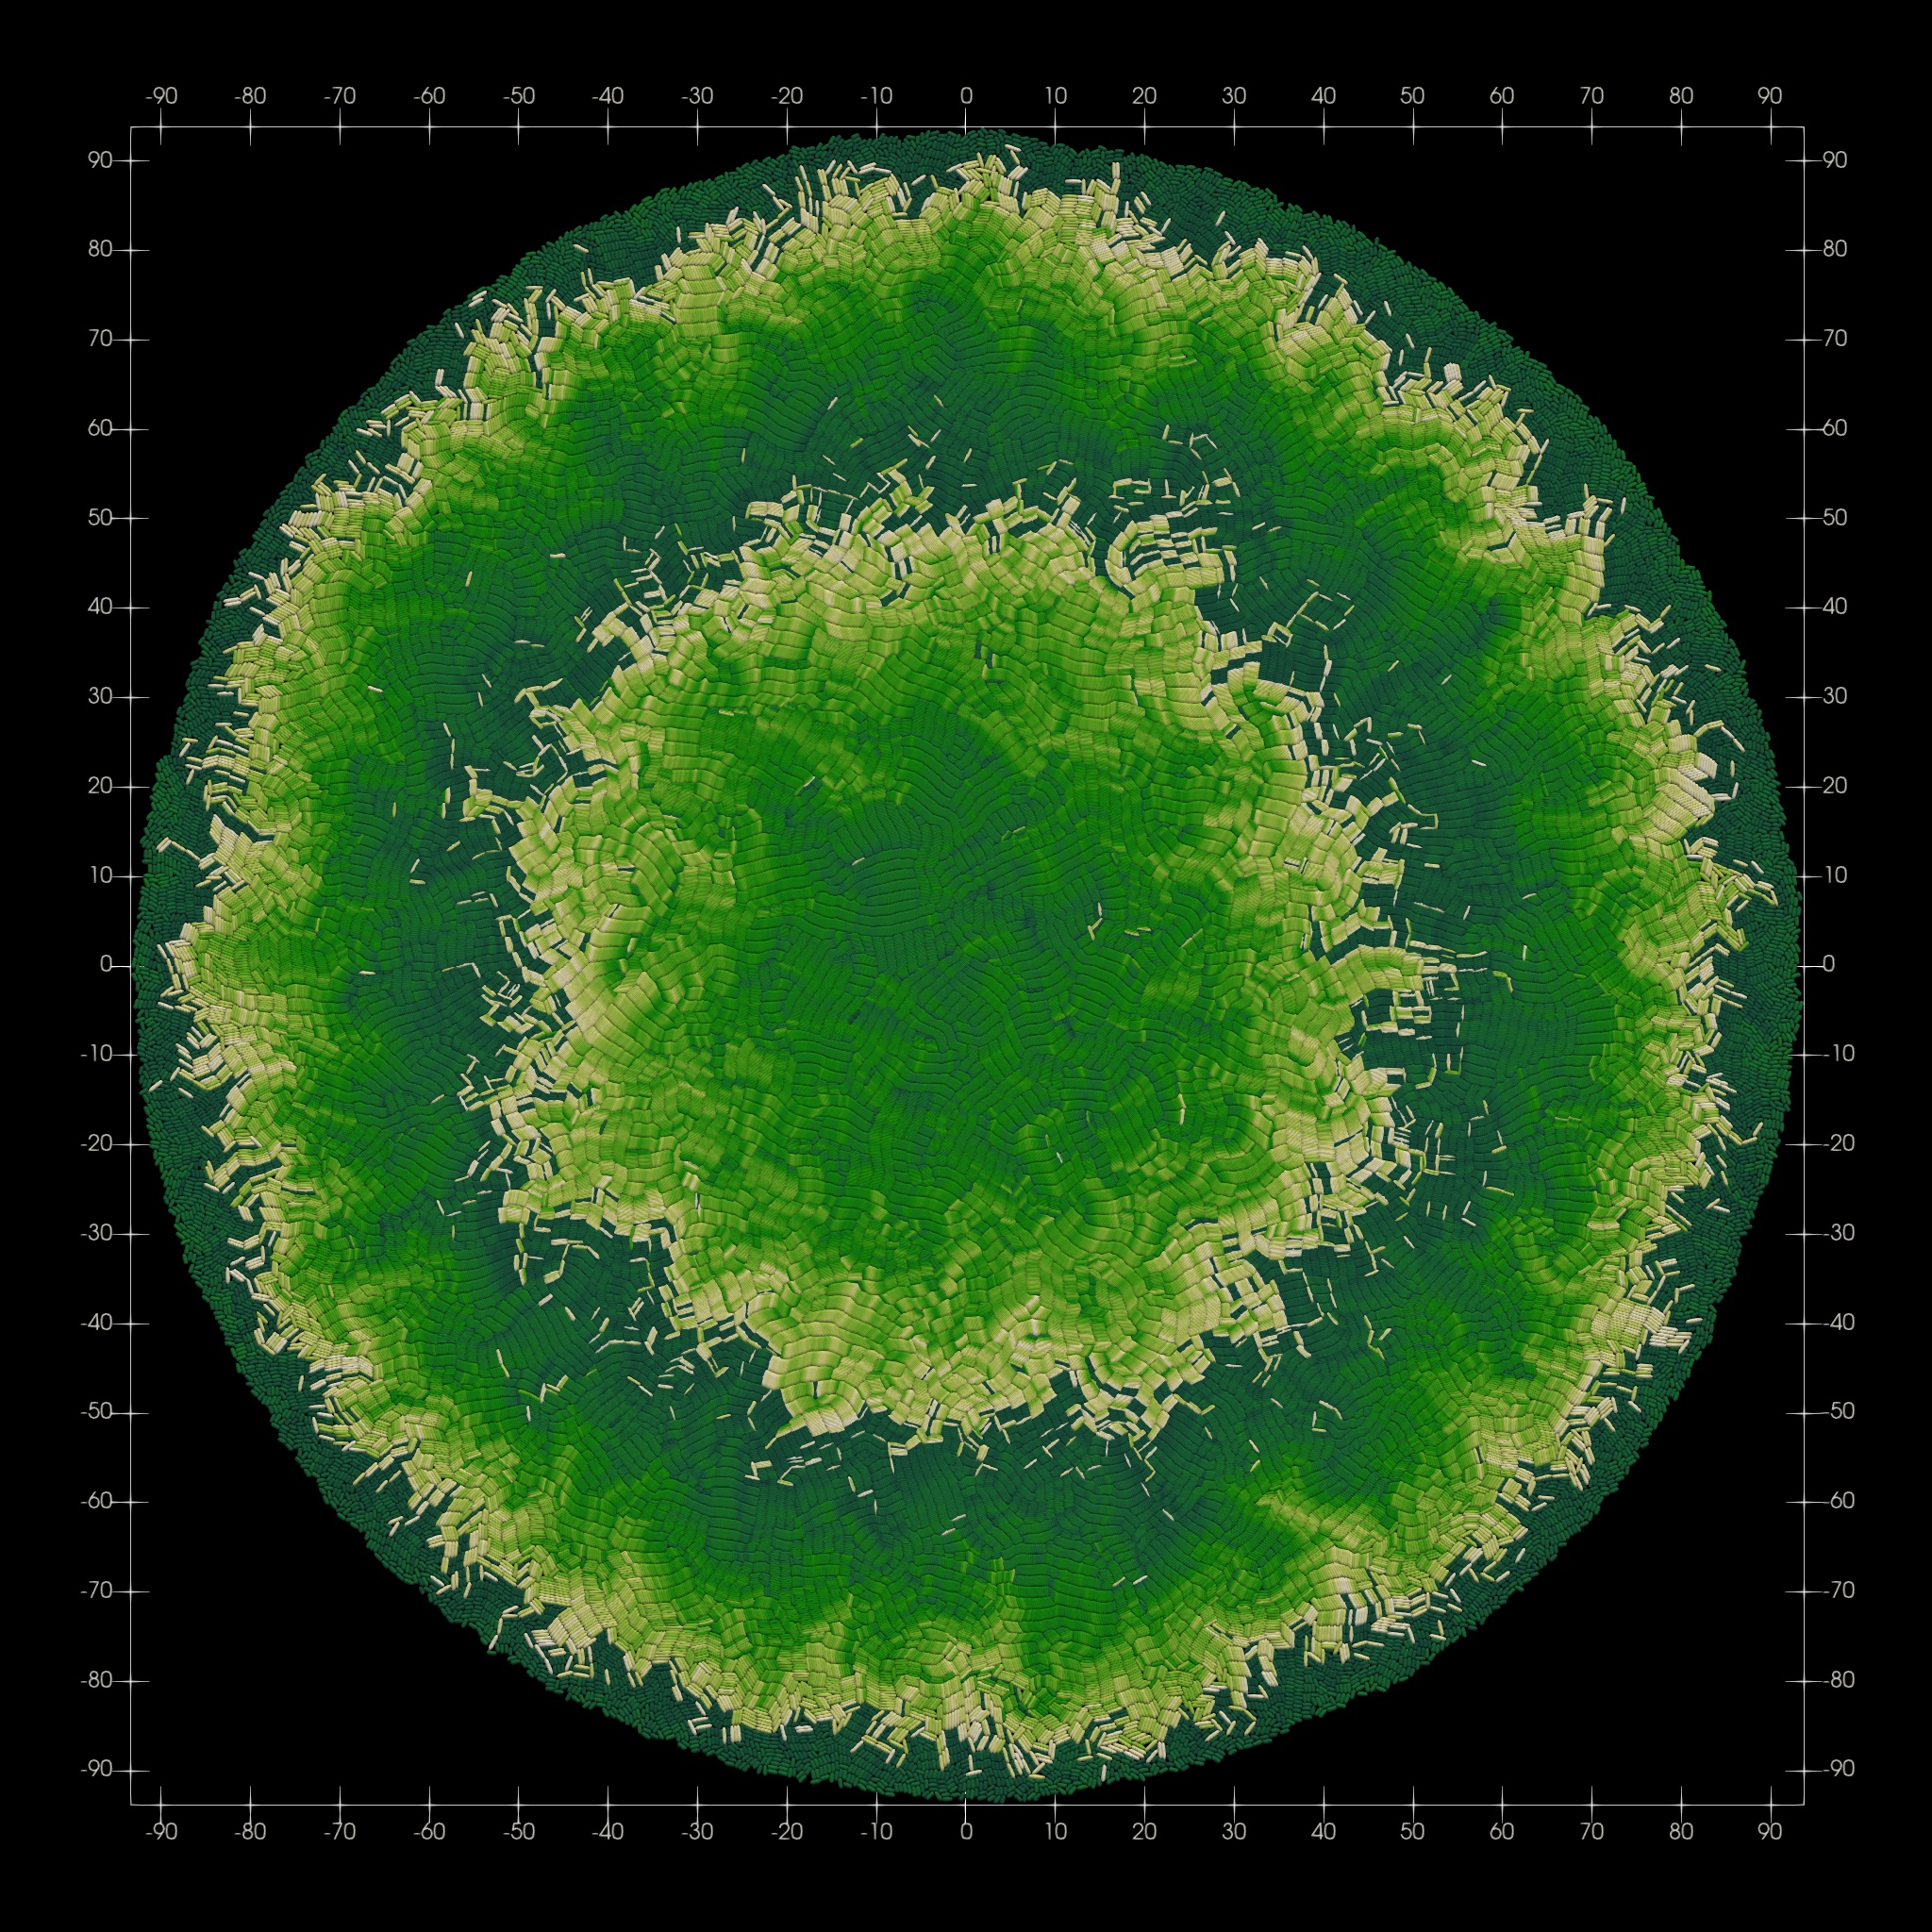
\includegraphics[width=0.25\textwidth]{figures/figures_paper/growth/soft_e-3/soft_e-3.0187.jpeg} &
%             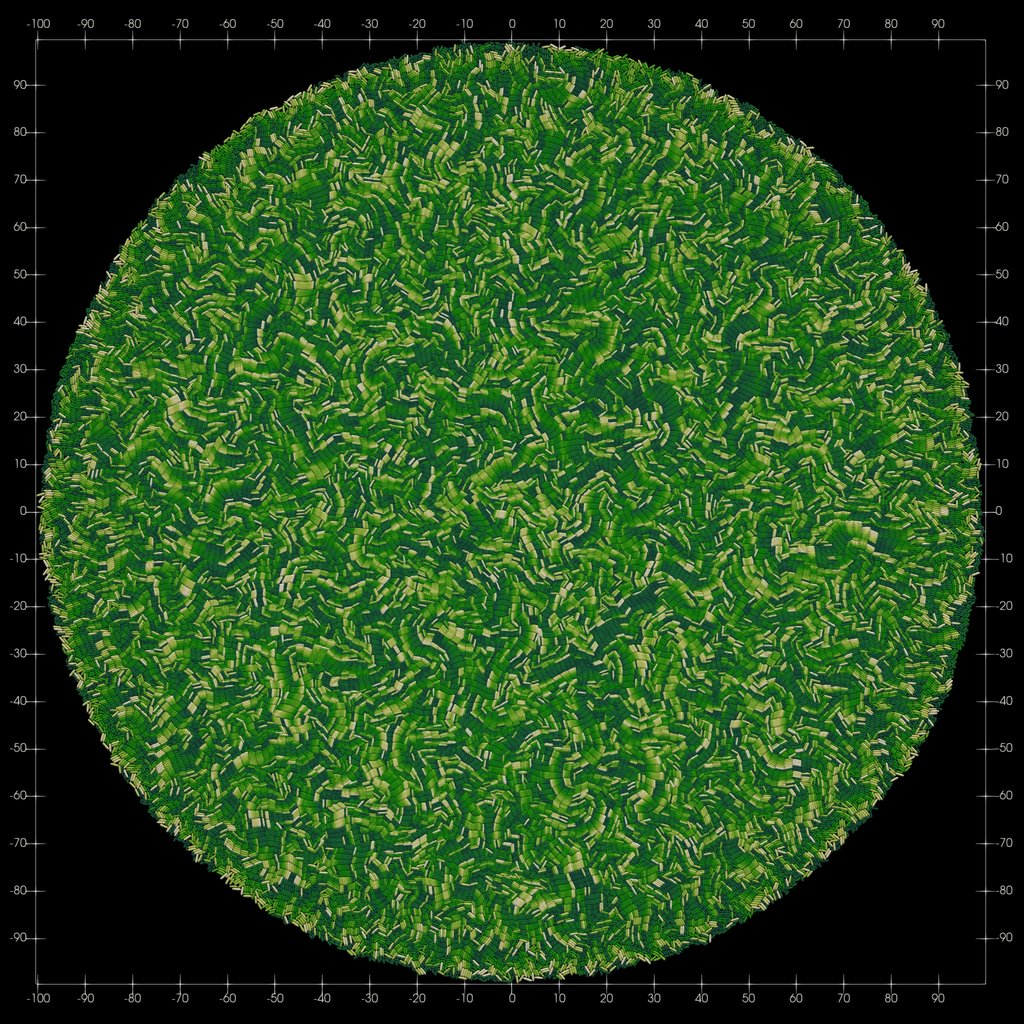
\includegraphics[width=0.25\textwidth]{figures/figures_paper/growth/soft_e-2/soft_e-2.0200.jpeg}                                                                                          \\[3pt]

%                                                                                                              & \scriptsize{No inhibition} & \scriptsize{Clear rings} & \scriptsize{Strong inhibition}
%         \end{tabular}
%     \end{figure}

% \end{frame}

\begin{frame}
    \frametitle{Critical Difference: Packing Density}

    \begin{columns}
        \begin{column}{0.5\textwidth}
            \begin{figure}
                \centering
                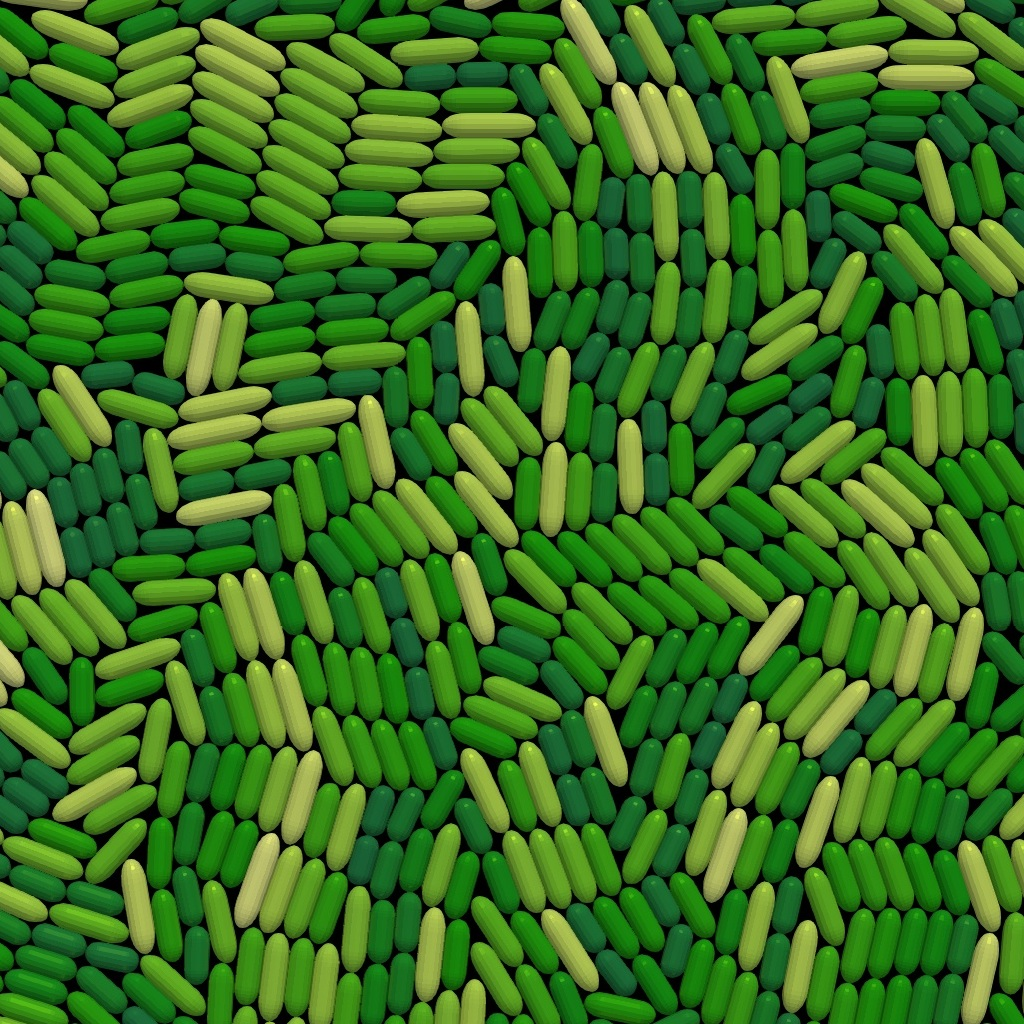
\includegraphics[width=0.9\textwidth]{figures/figures_paper/comparison_plots/density_hard.jpeg}
                \caption*{\textbf{Hard Model}}
            \end{figure}
        \end{column}

        \begin{column}{0.5\textwidth}
            \begin{figure}
                \centering
                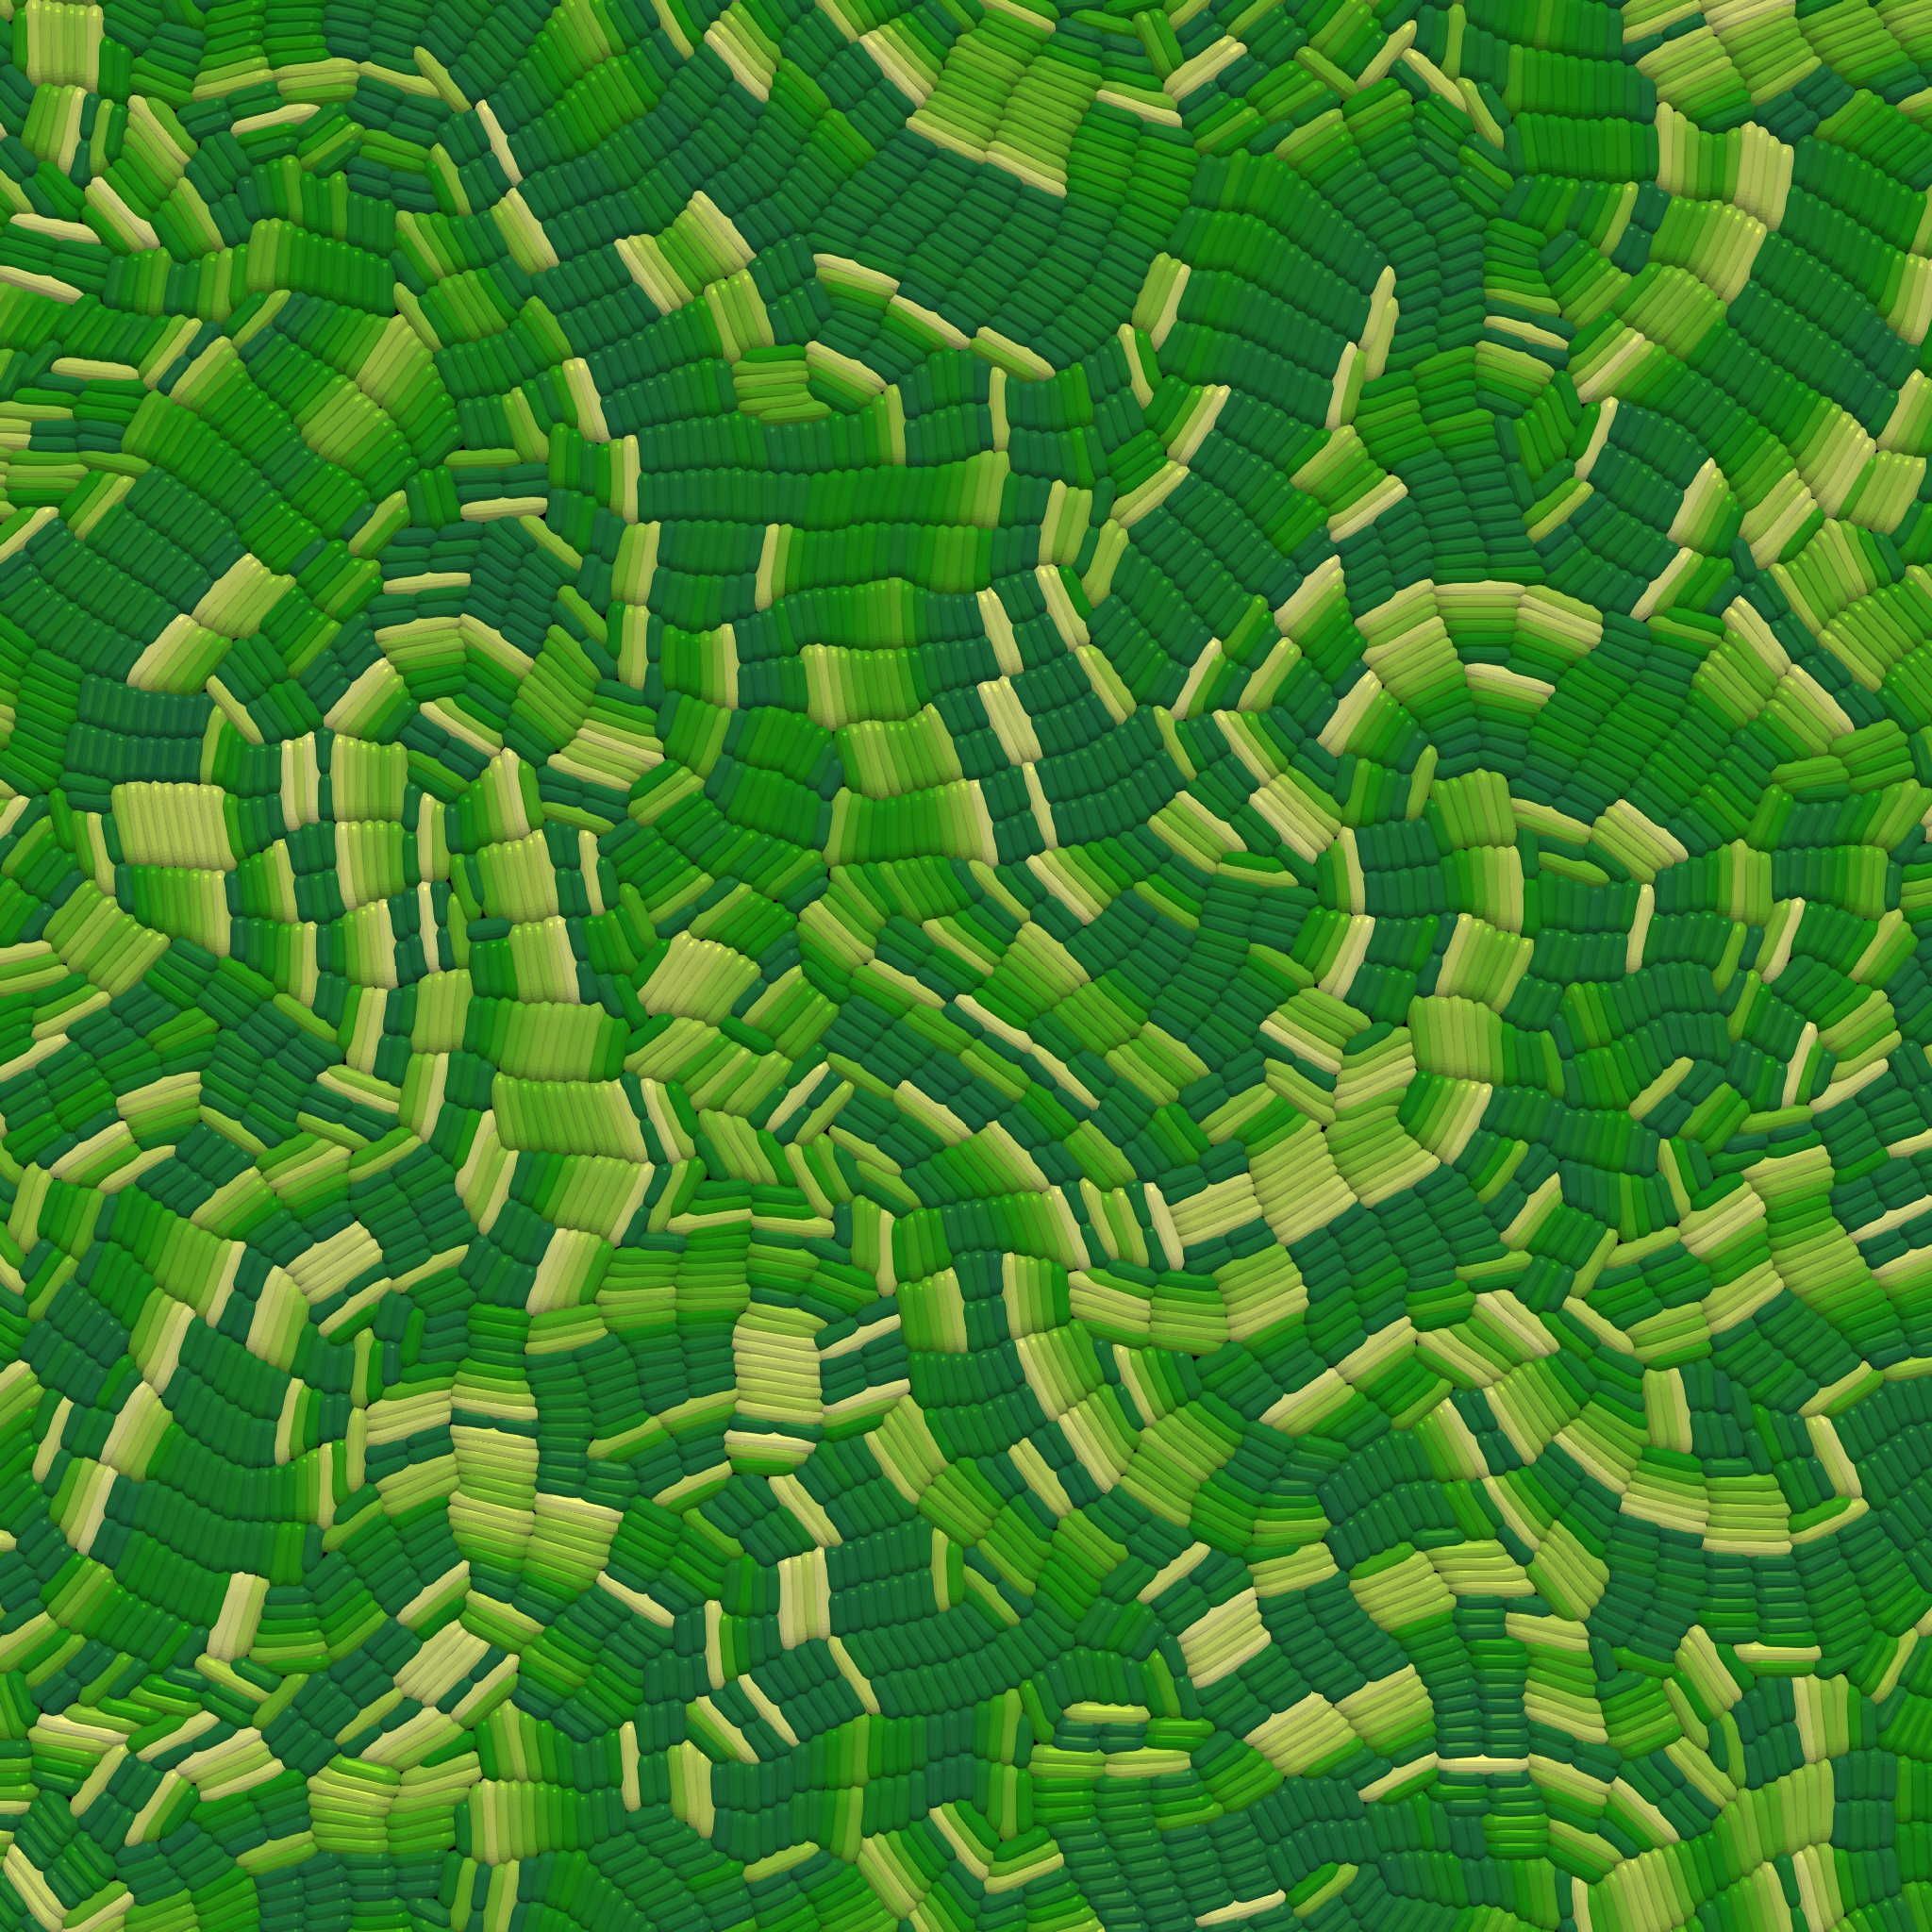
\includegraphics[width=0.9\textwidth]{figures/figures_paper/comparison_plots/density_soft.jpeg}
                \caption*{\textbf{Soft Model}}
            \end{figure}
        \end{column}
    \end{columns}

\end{frame}


\begin{frame}
    \frametitle{Critical Difference: Microdomain Structure}

    \begin{columns}
        \begin{column}{0.5\textwidth}
            \begin{figure}
                \centering
                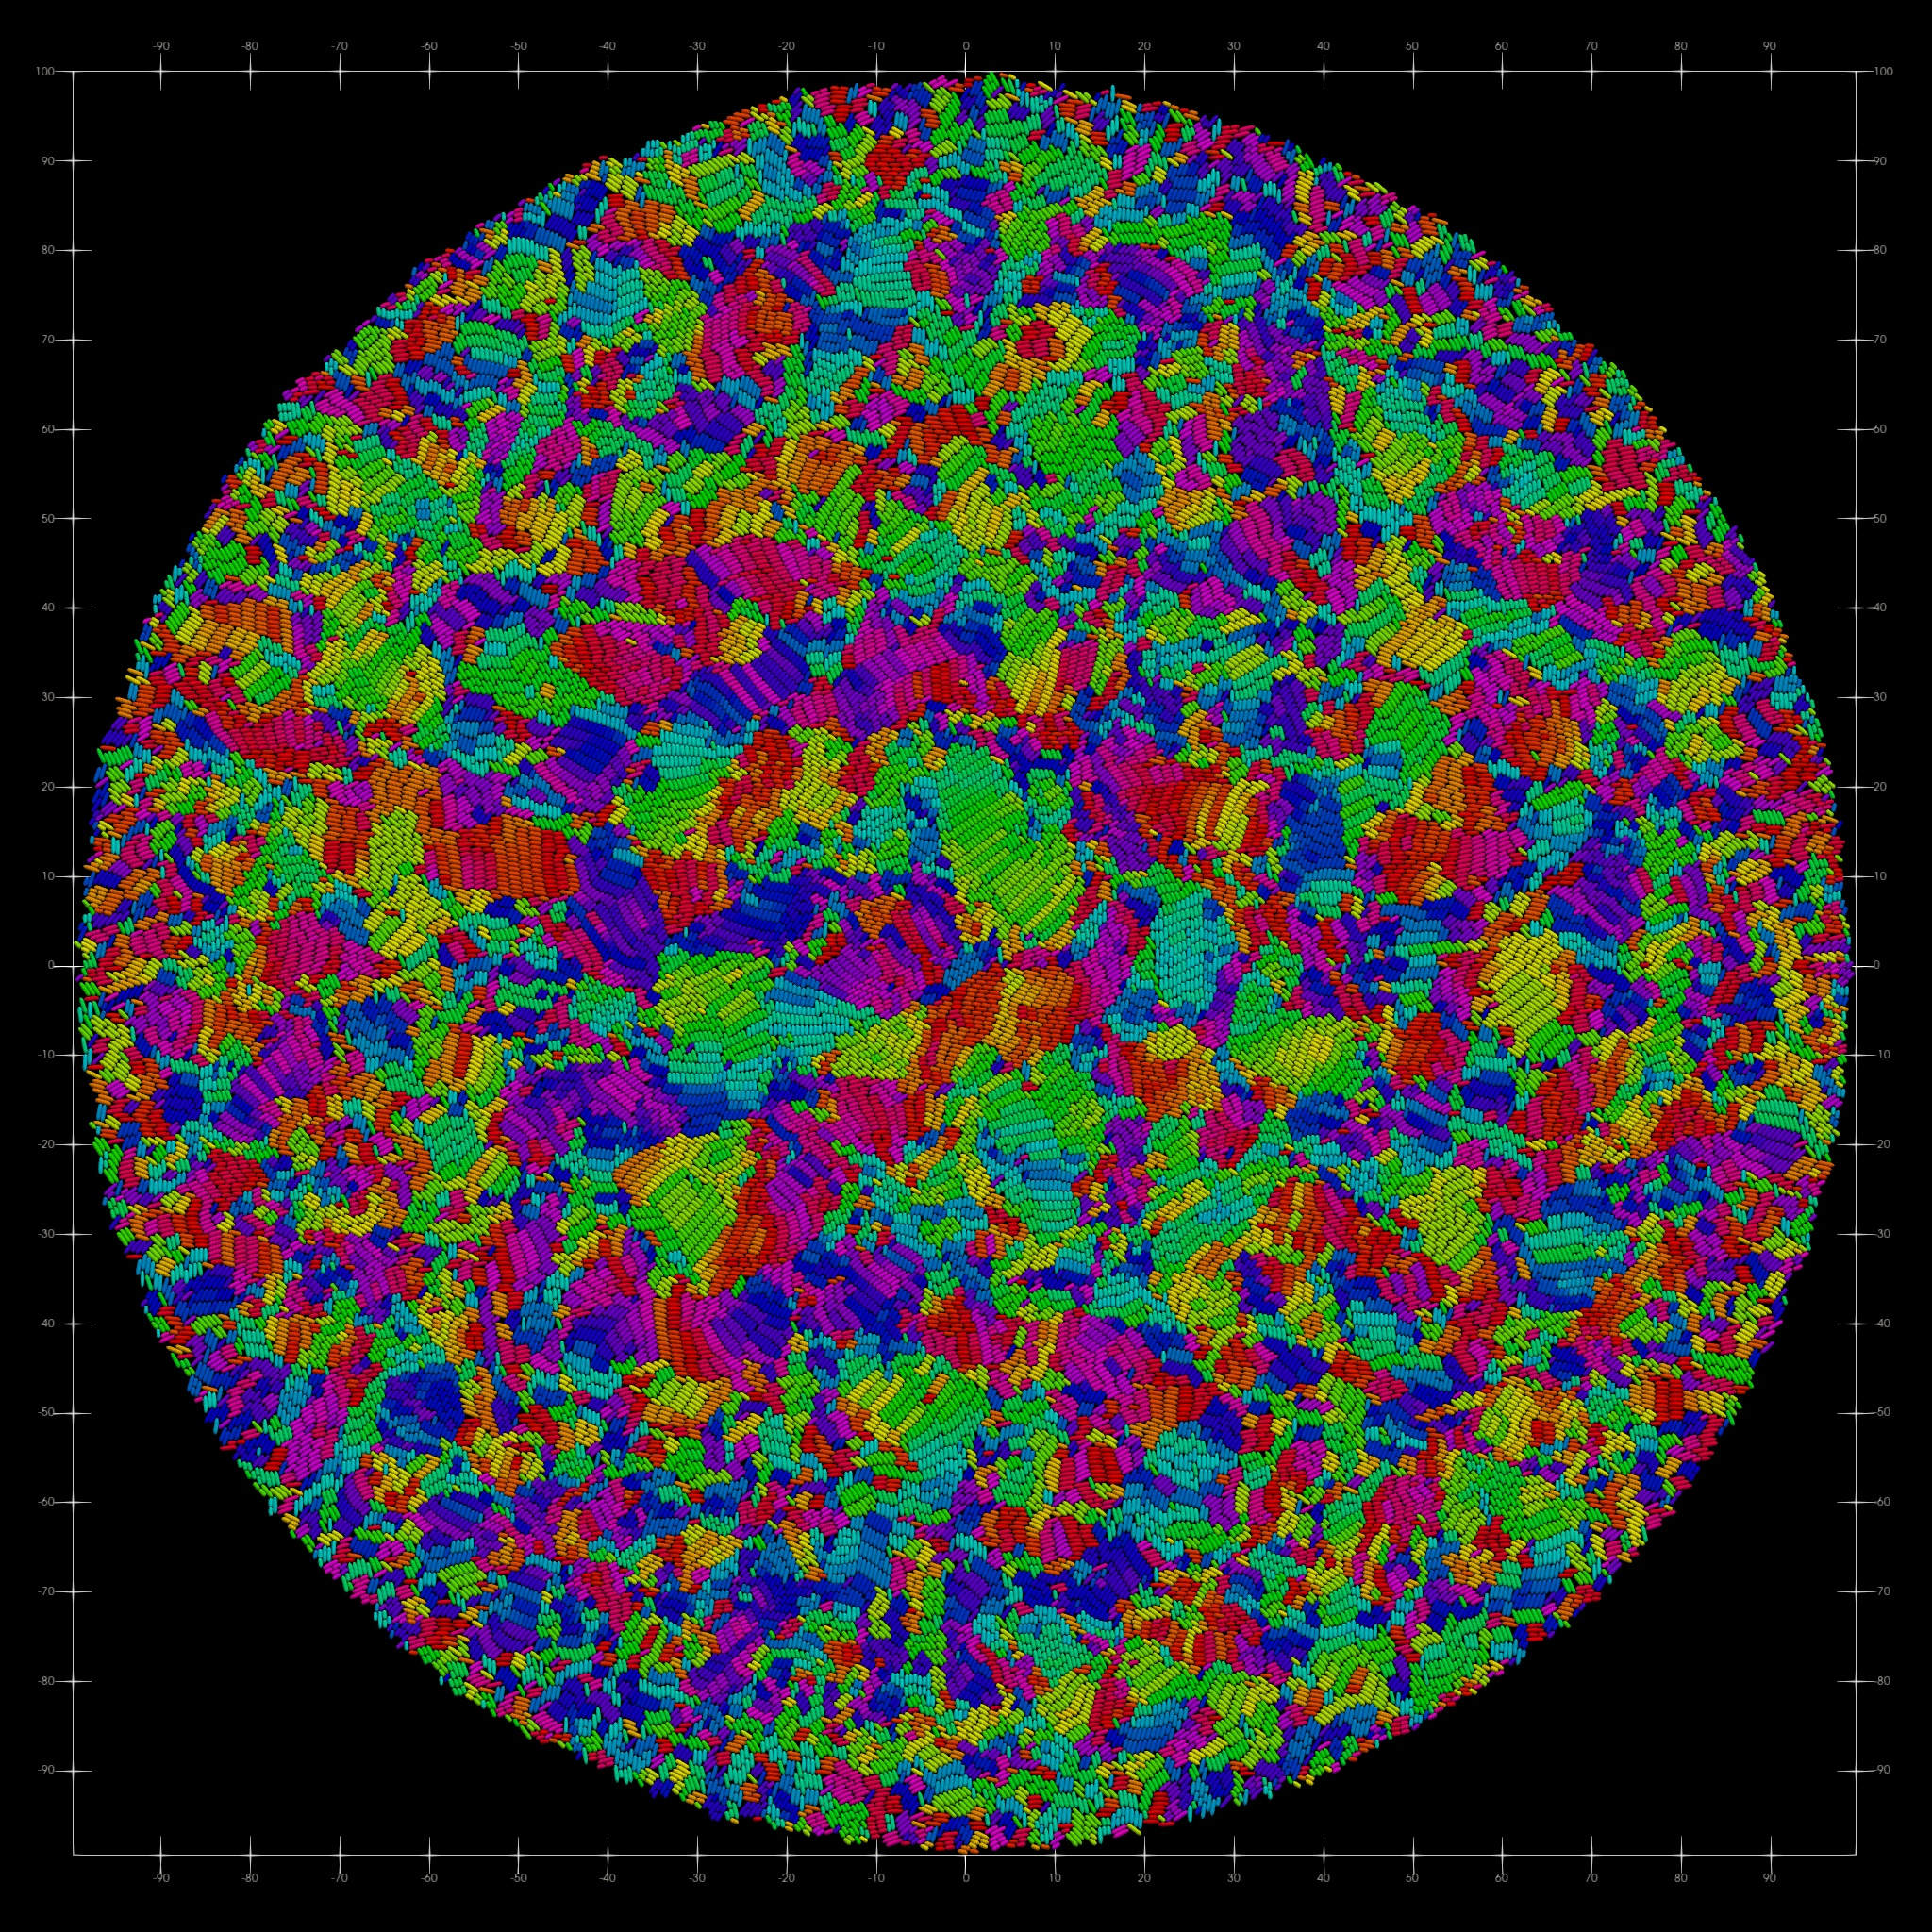
\includegraphics[width=0.9\textwidth]{figures/figures_paper/orientation_comparisons/zoomed_images/hard_e-3_orient.jpeg}
                \caption*{\textbf{Hard: realistic patches }}
            \end{figure}
        \end{column}

        \begin{column}{0.5\textwidth}
            \begin{figure}
                \centering
                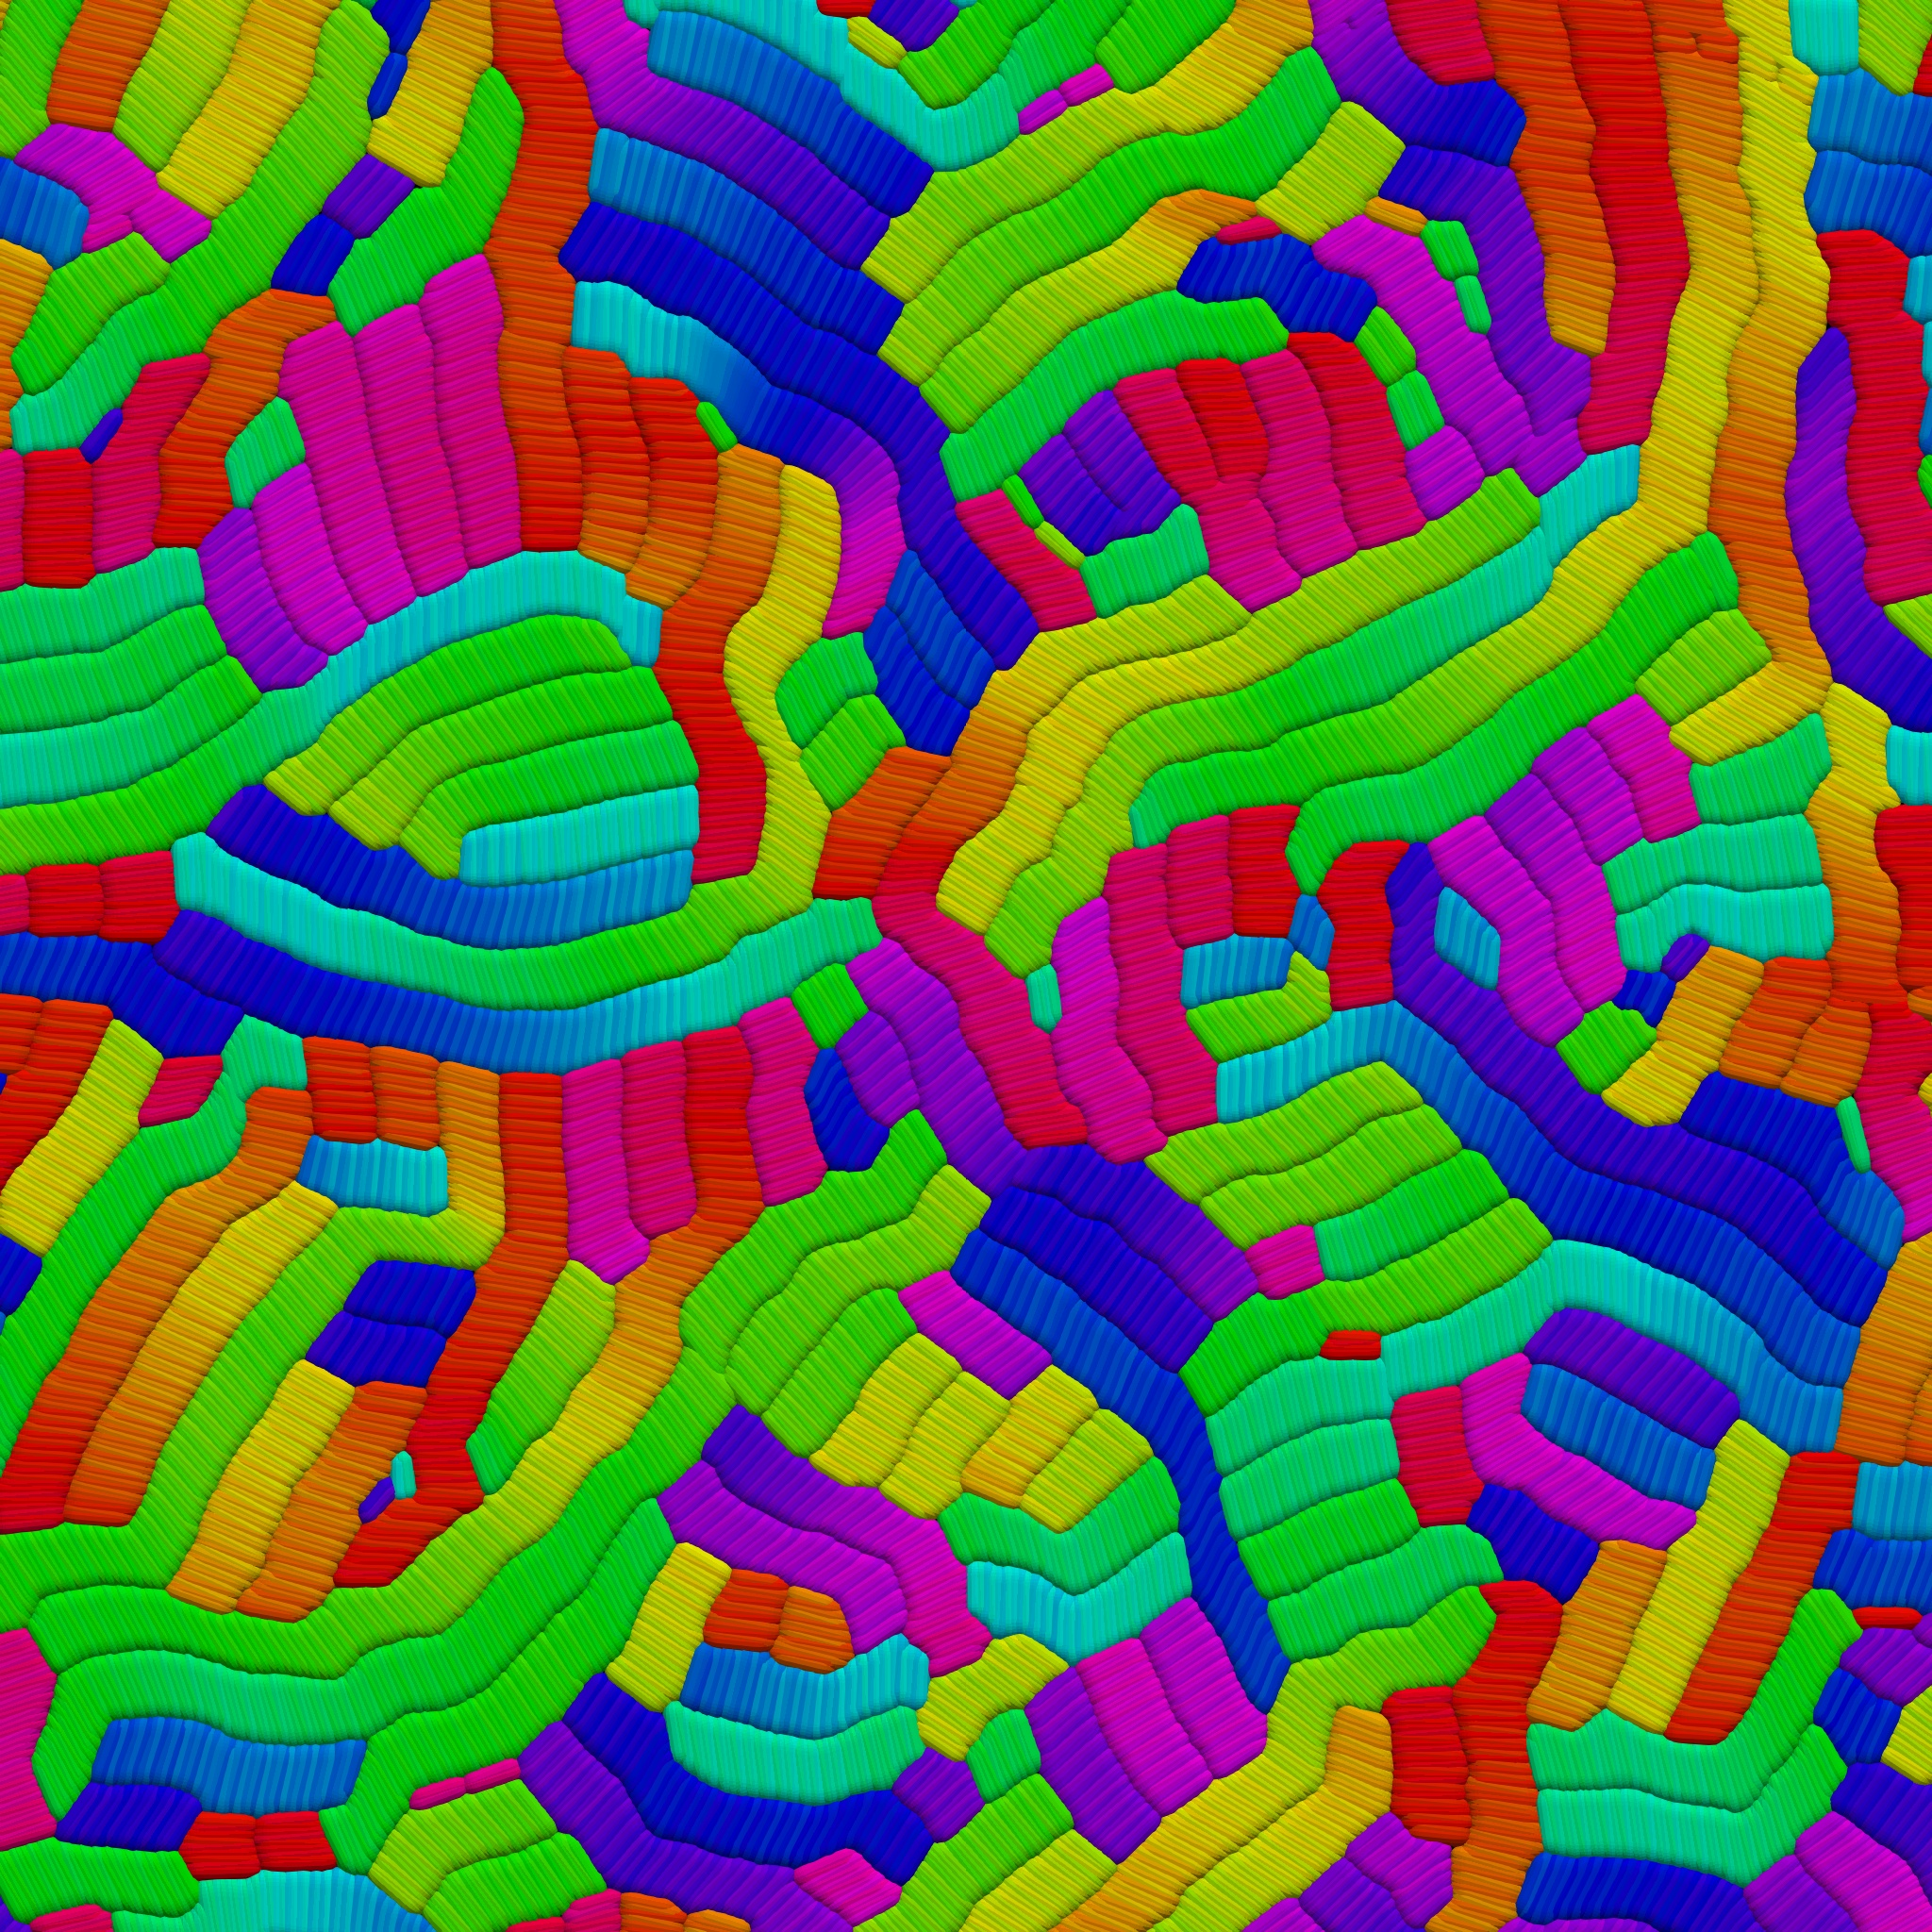
\includegraphics[width=0.9\textwidth]{figures/figures_paper/orientation_comparisons/zoomed_images/soft_e-3_orient.jpeg}
                \caption*{\textbf{Soft: elongated bundles }}
            \end{figure}
        \end{column}
    \end{columns}

\end{frame}

% ============================================================
% SECTION 6: COMPUTATIONAL PERFORMANCE
% ============================================================

\section{Computational Performance}

\begin{frame}
    \frametitle{CFL Condition}

    \vspace{0.5cm}

    \begin{columns}
        \begin{column}{0.52\textwidth}
            \textbf{Adaptive timestepping:}
            \begin{equation*}
                \Delta t = \frac{0.5 \, \varepsilon}{u_m}
            \end{equation*}

            \vspace{-0.5cm}

            \begin{equation*}
                \begin{align}
                    \text{where }   u_m & = \text{median velocity},  \\
                    \varepsilon         & = \text{overlap tolerance}
                \end{align}
            \end{equation*}

            \textbf{Key observations:}
            \begin{itemize}
                \item Hard: stable $\Delta t \sim 3 \cdot 10^{-4}$
                \item Soft: drops $\Delta t \sim 10^{-5}$
                \item $30\times$ larger timesteps!
            \end{itemize}
        \end{column}

        \begin{column}{0.52\textwidth}
            \begin{figure}
                \centering
                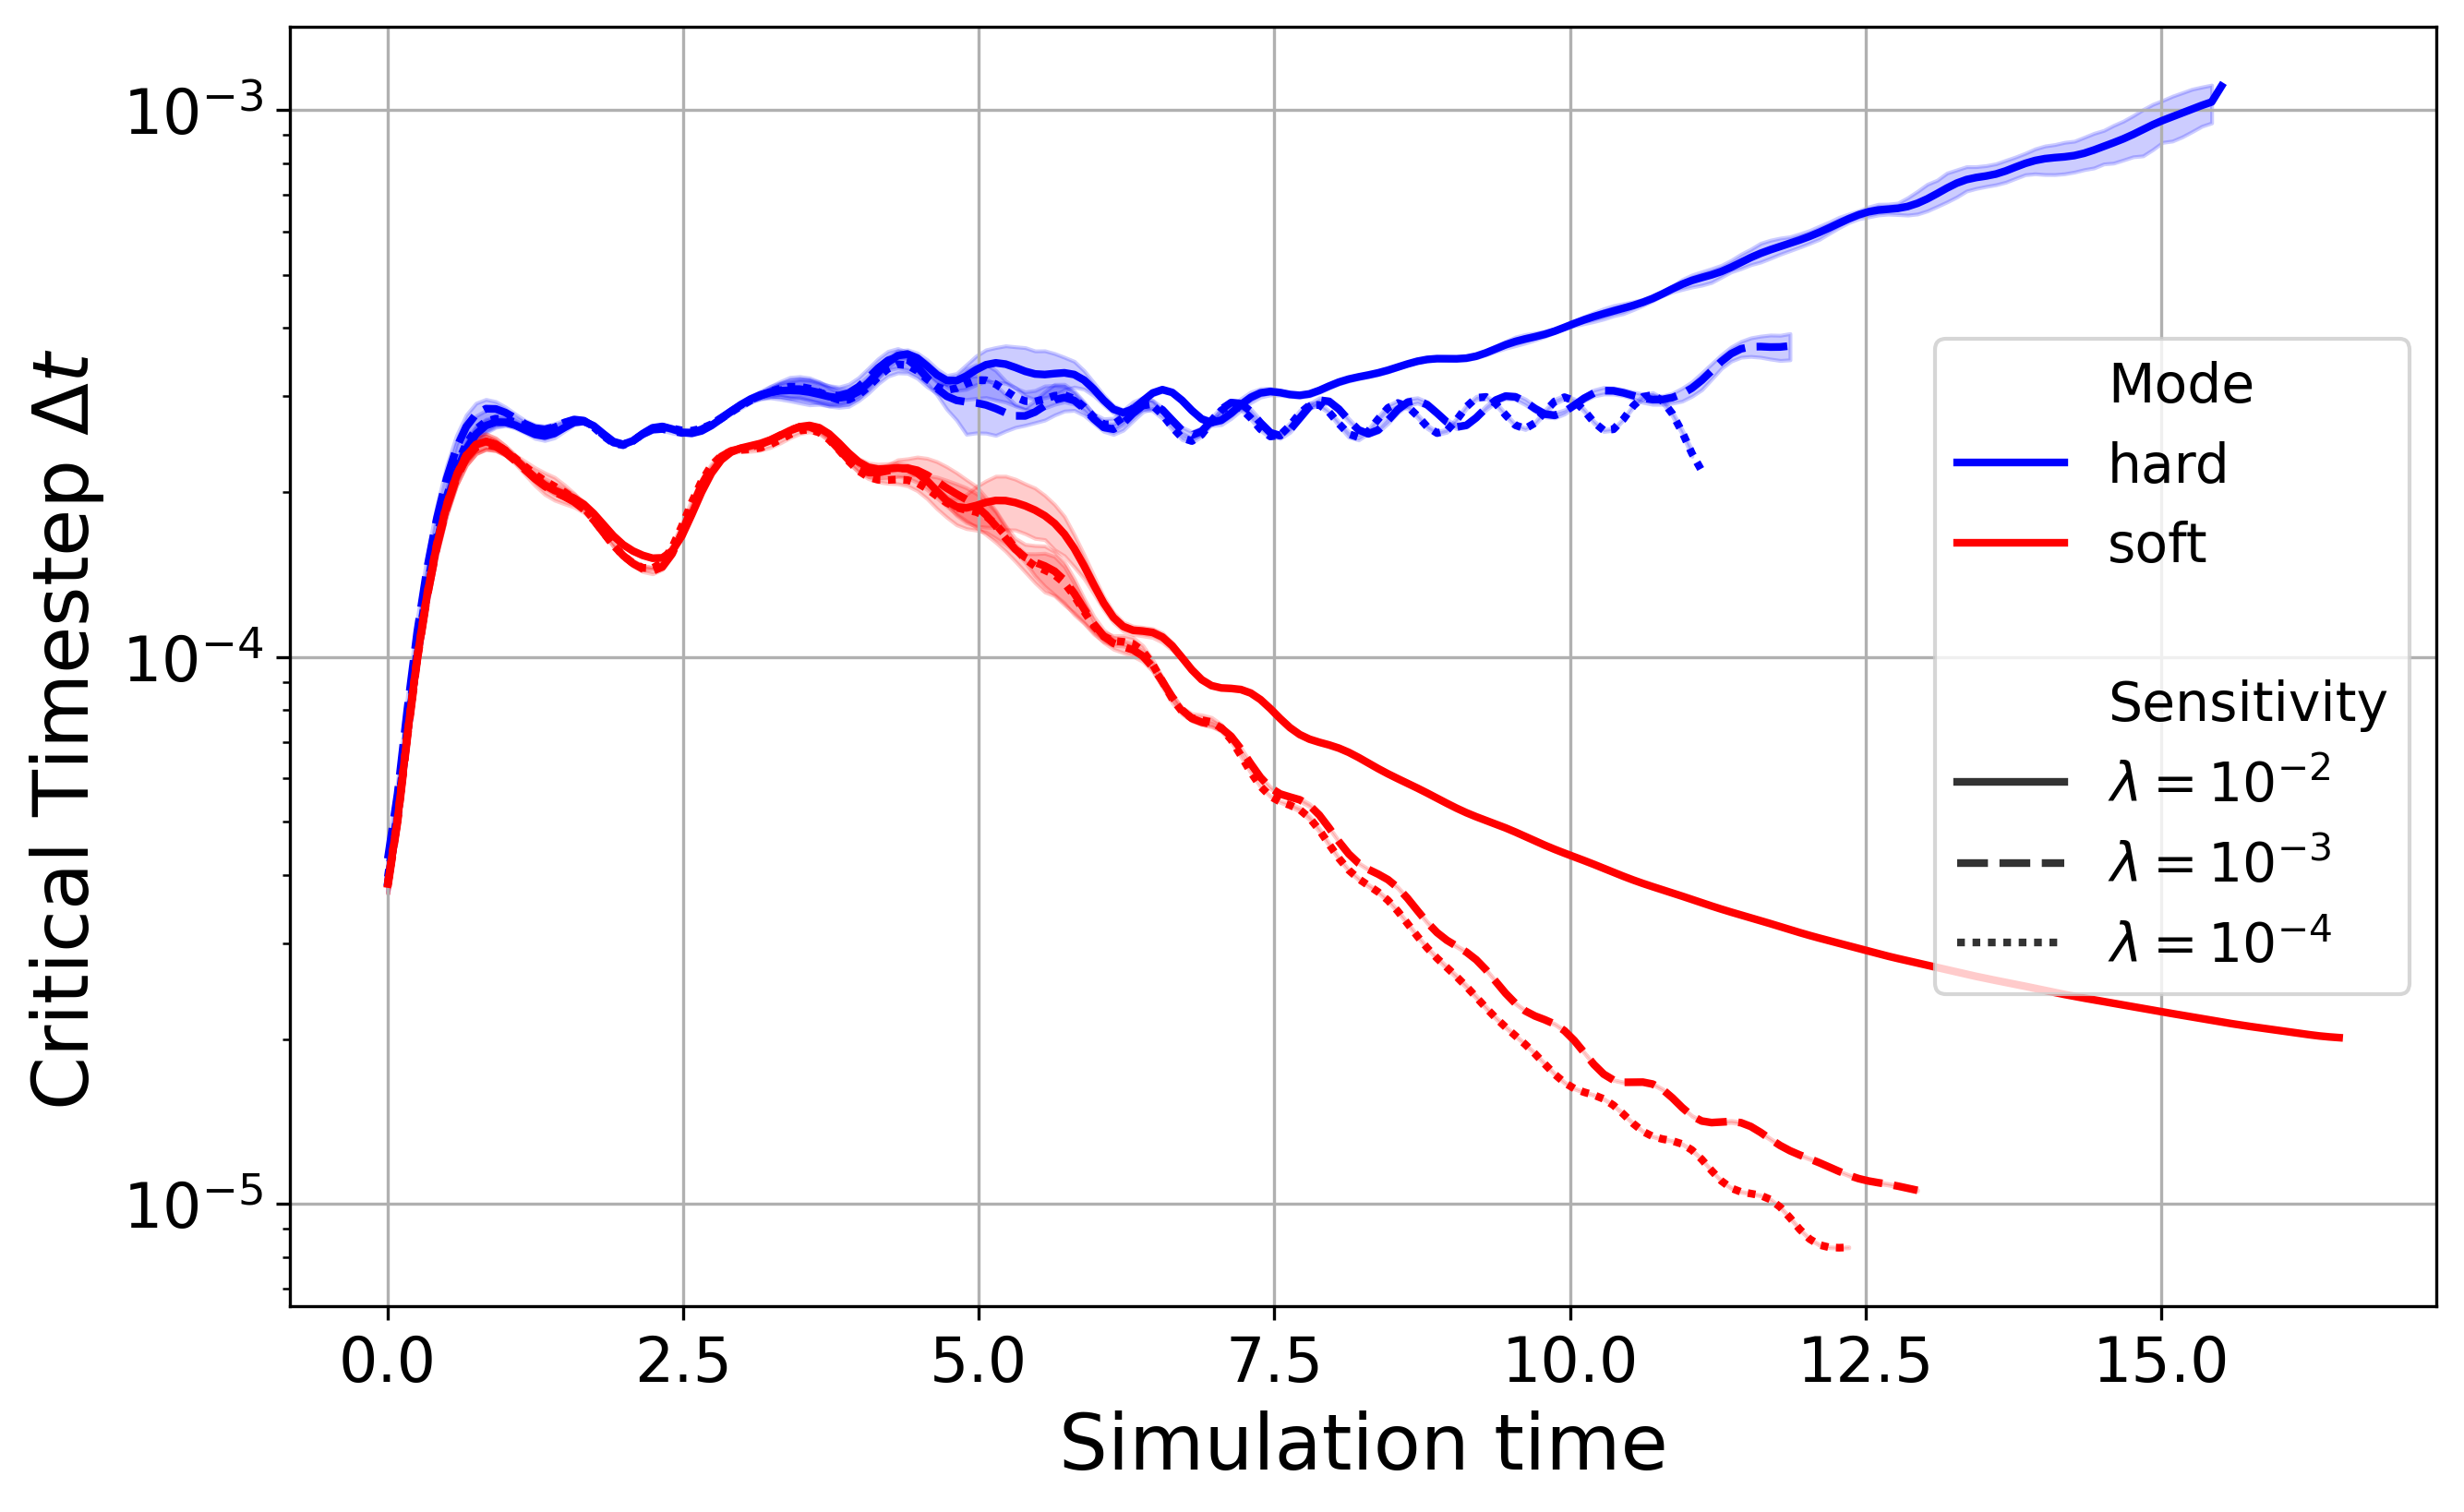
\includegraphics[width=\textwidth]{figures/figures_paper/comparison_plots/combined_simulation_time_vs_dt.png}
            \end{figure}
        \end{column}
    \end{columns}

\end{frame}

\begin{frame}
    \frametitle{Parallel Architecture}

    \begin{columns}[c]
        \begin{column}{0.5\textwidth}
            \textbf{Implementation:}
            \begin{itemize}
                \item MPI + PETSc framework
                \item Distributed vectors/matrices
                \item Angular sector decomposition
                \item Ghost particle exchange
            \end{itemize}
        \end{column}

        \begin{column}{0.5\textwidth}
            \vspace{-0.3cm}
            \begin{figure}
                \centering
                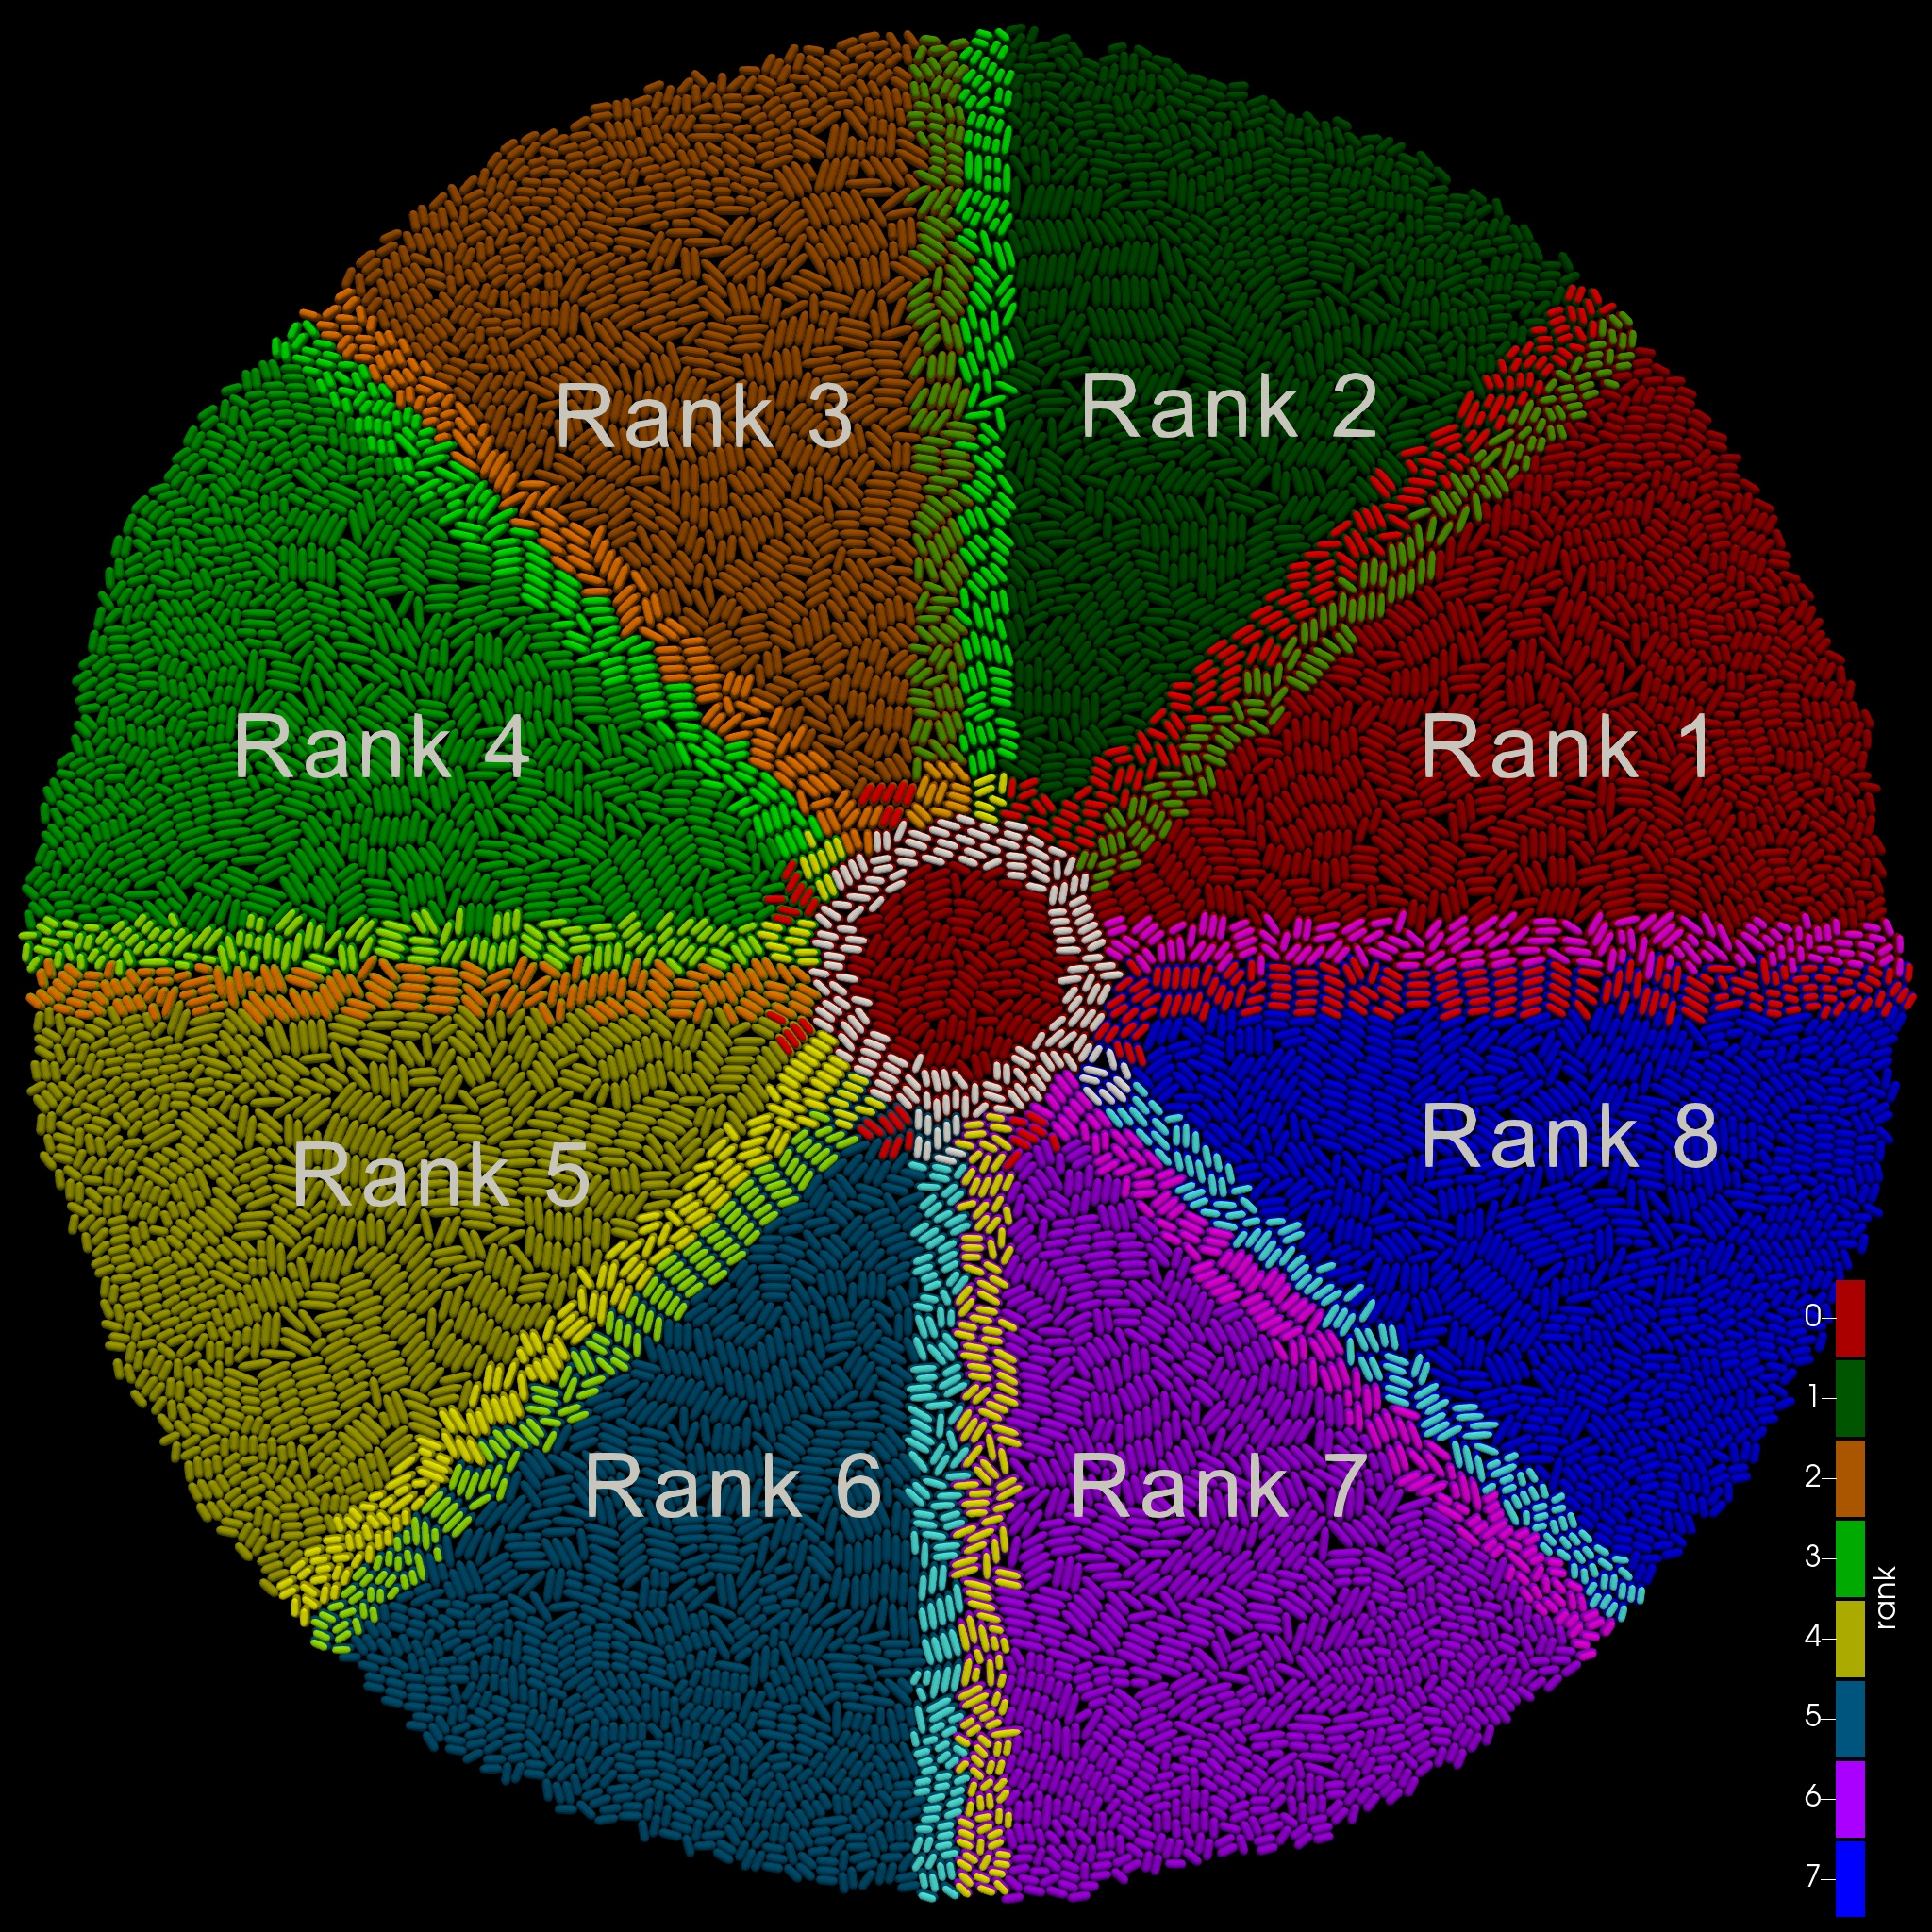
\includegraphics[width=\textwidth]{figures/figures_paper/runtimes/domain_decomposition.jpeg}
                \caption*{\scriptsize{Domain decomposition with 8 MPI ranks}}
            \end{figure}
        \end{column}
    \end{columns}

\end{frame}

\begin{frame}
    \frametitle{Strong Scaling: Runtime to reach $R=100$}

    \begin{figure}
        \centering
        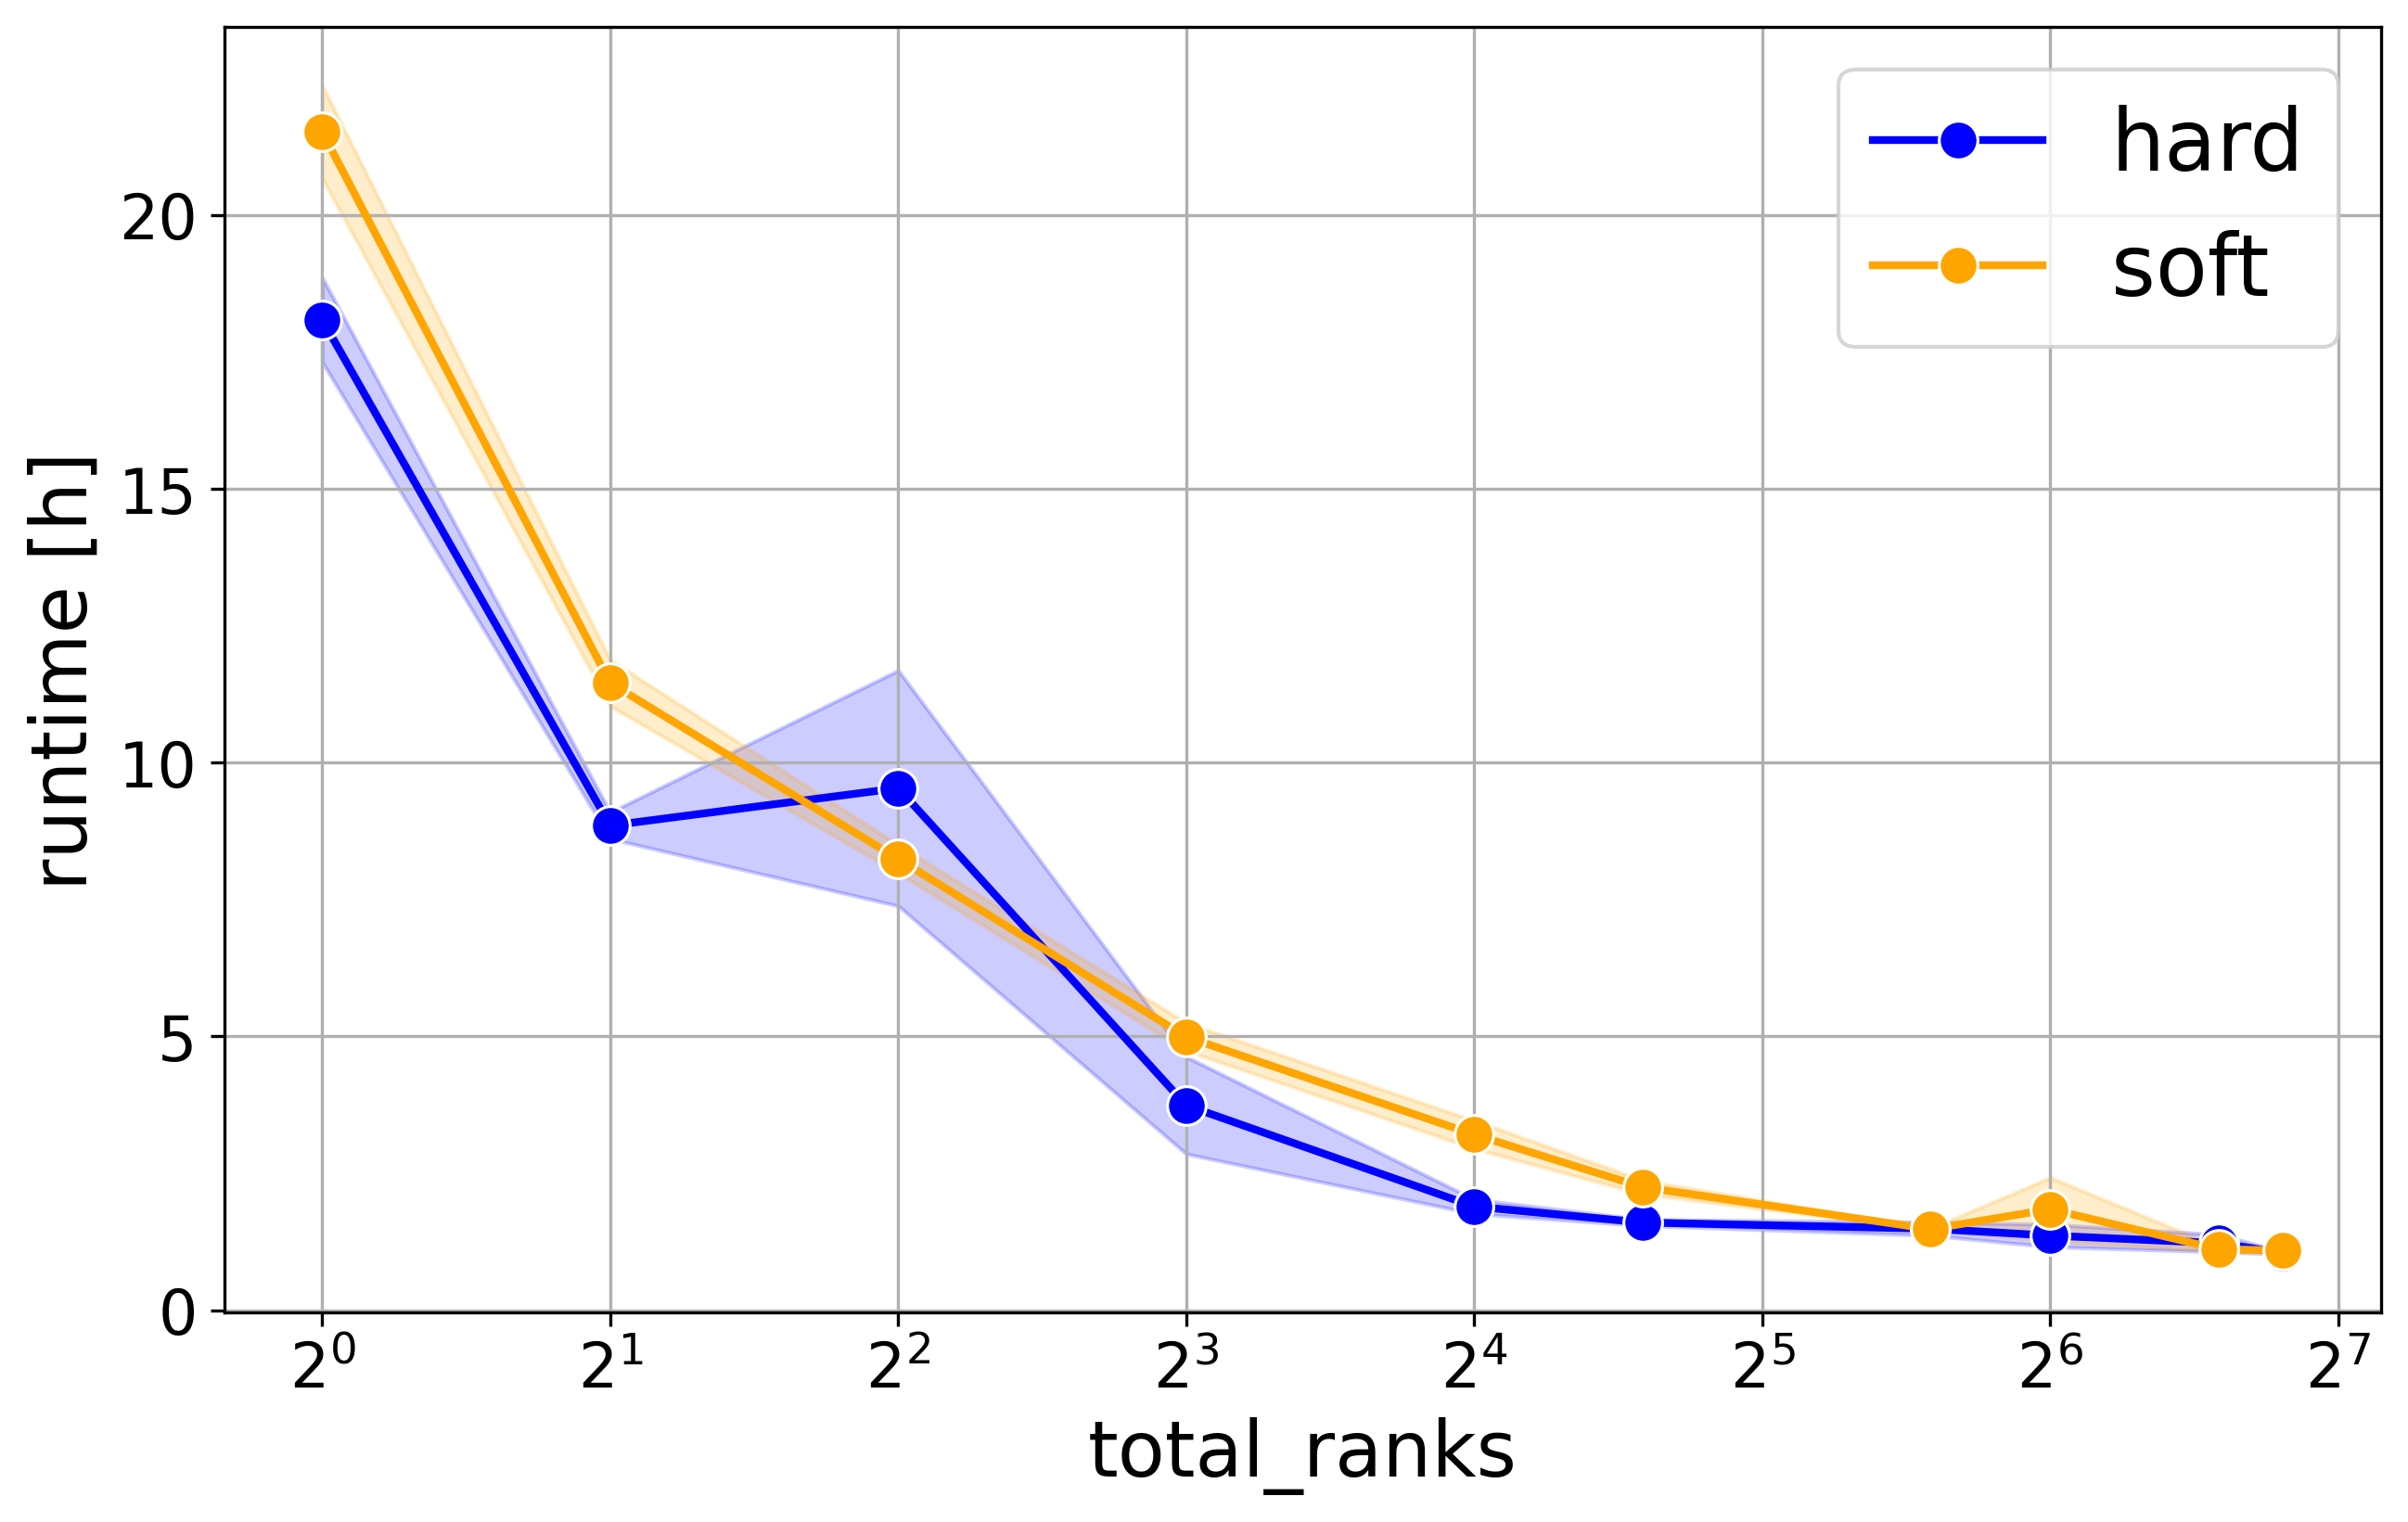
\includegraphics[width=0.8\textwidth]{figures/figures_paper/runtimes/strong_scaling_runtime_hard_soft.png}
    \end{figure}

    \begin{itemize}
        \item Hard model is always faster!
        \item Huge communication overhead (Especially for small $\Delta t$)
    \end{itemize}

\end{frame}

% \begin{frame}
%     \frametitle{Maximum Colony Size (24h budget, 112 cores)}

%     \begin{columns}
%         \begin{column}{0.45\textwidth}
%             \textbf{Hard Model:}
%             \begin{itemize}
%                 \item $R_{\max} = 260$
%                 \item 301,116 cells
%                 \item Maintains accuracy
%             \end{itemize}

%             \vspace{0.2cm}

%             \textbf{Scaling:}
%             \begin{itemize}
%                 \item $T[h] \propto R^5 \propto N^{2.5}$
%                 \item $\mathcal{O}(N)$ BBPGD iterations per step
%                 \item Costly (sparse) matrix-vector products
%             \end{itemize}
%         \end{column}

%         \begin{column}{0.55\textwidth}
%             \begin{figure}
%                 \centering
%                 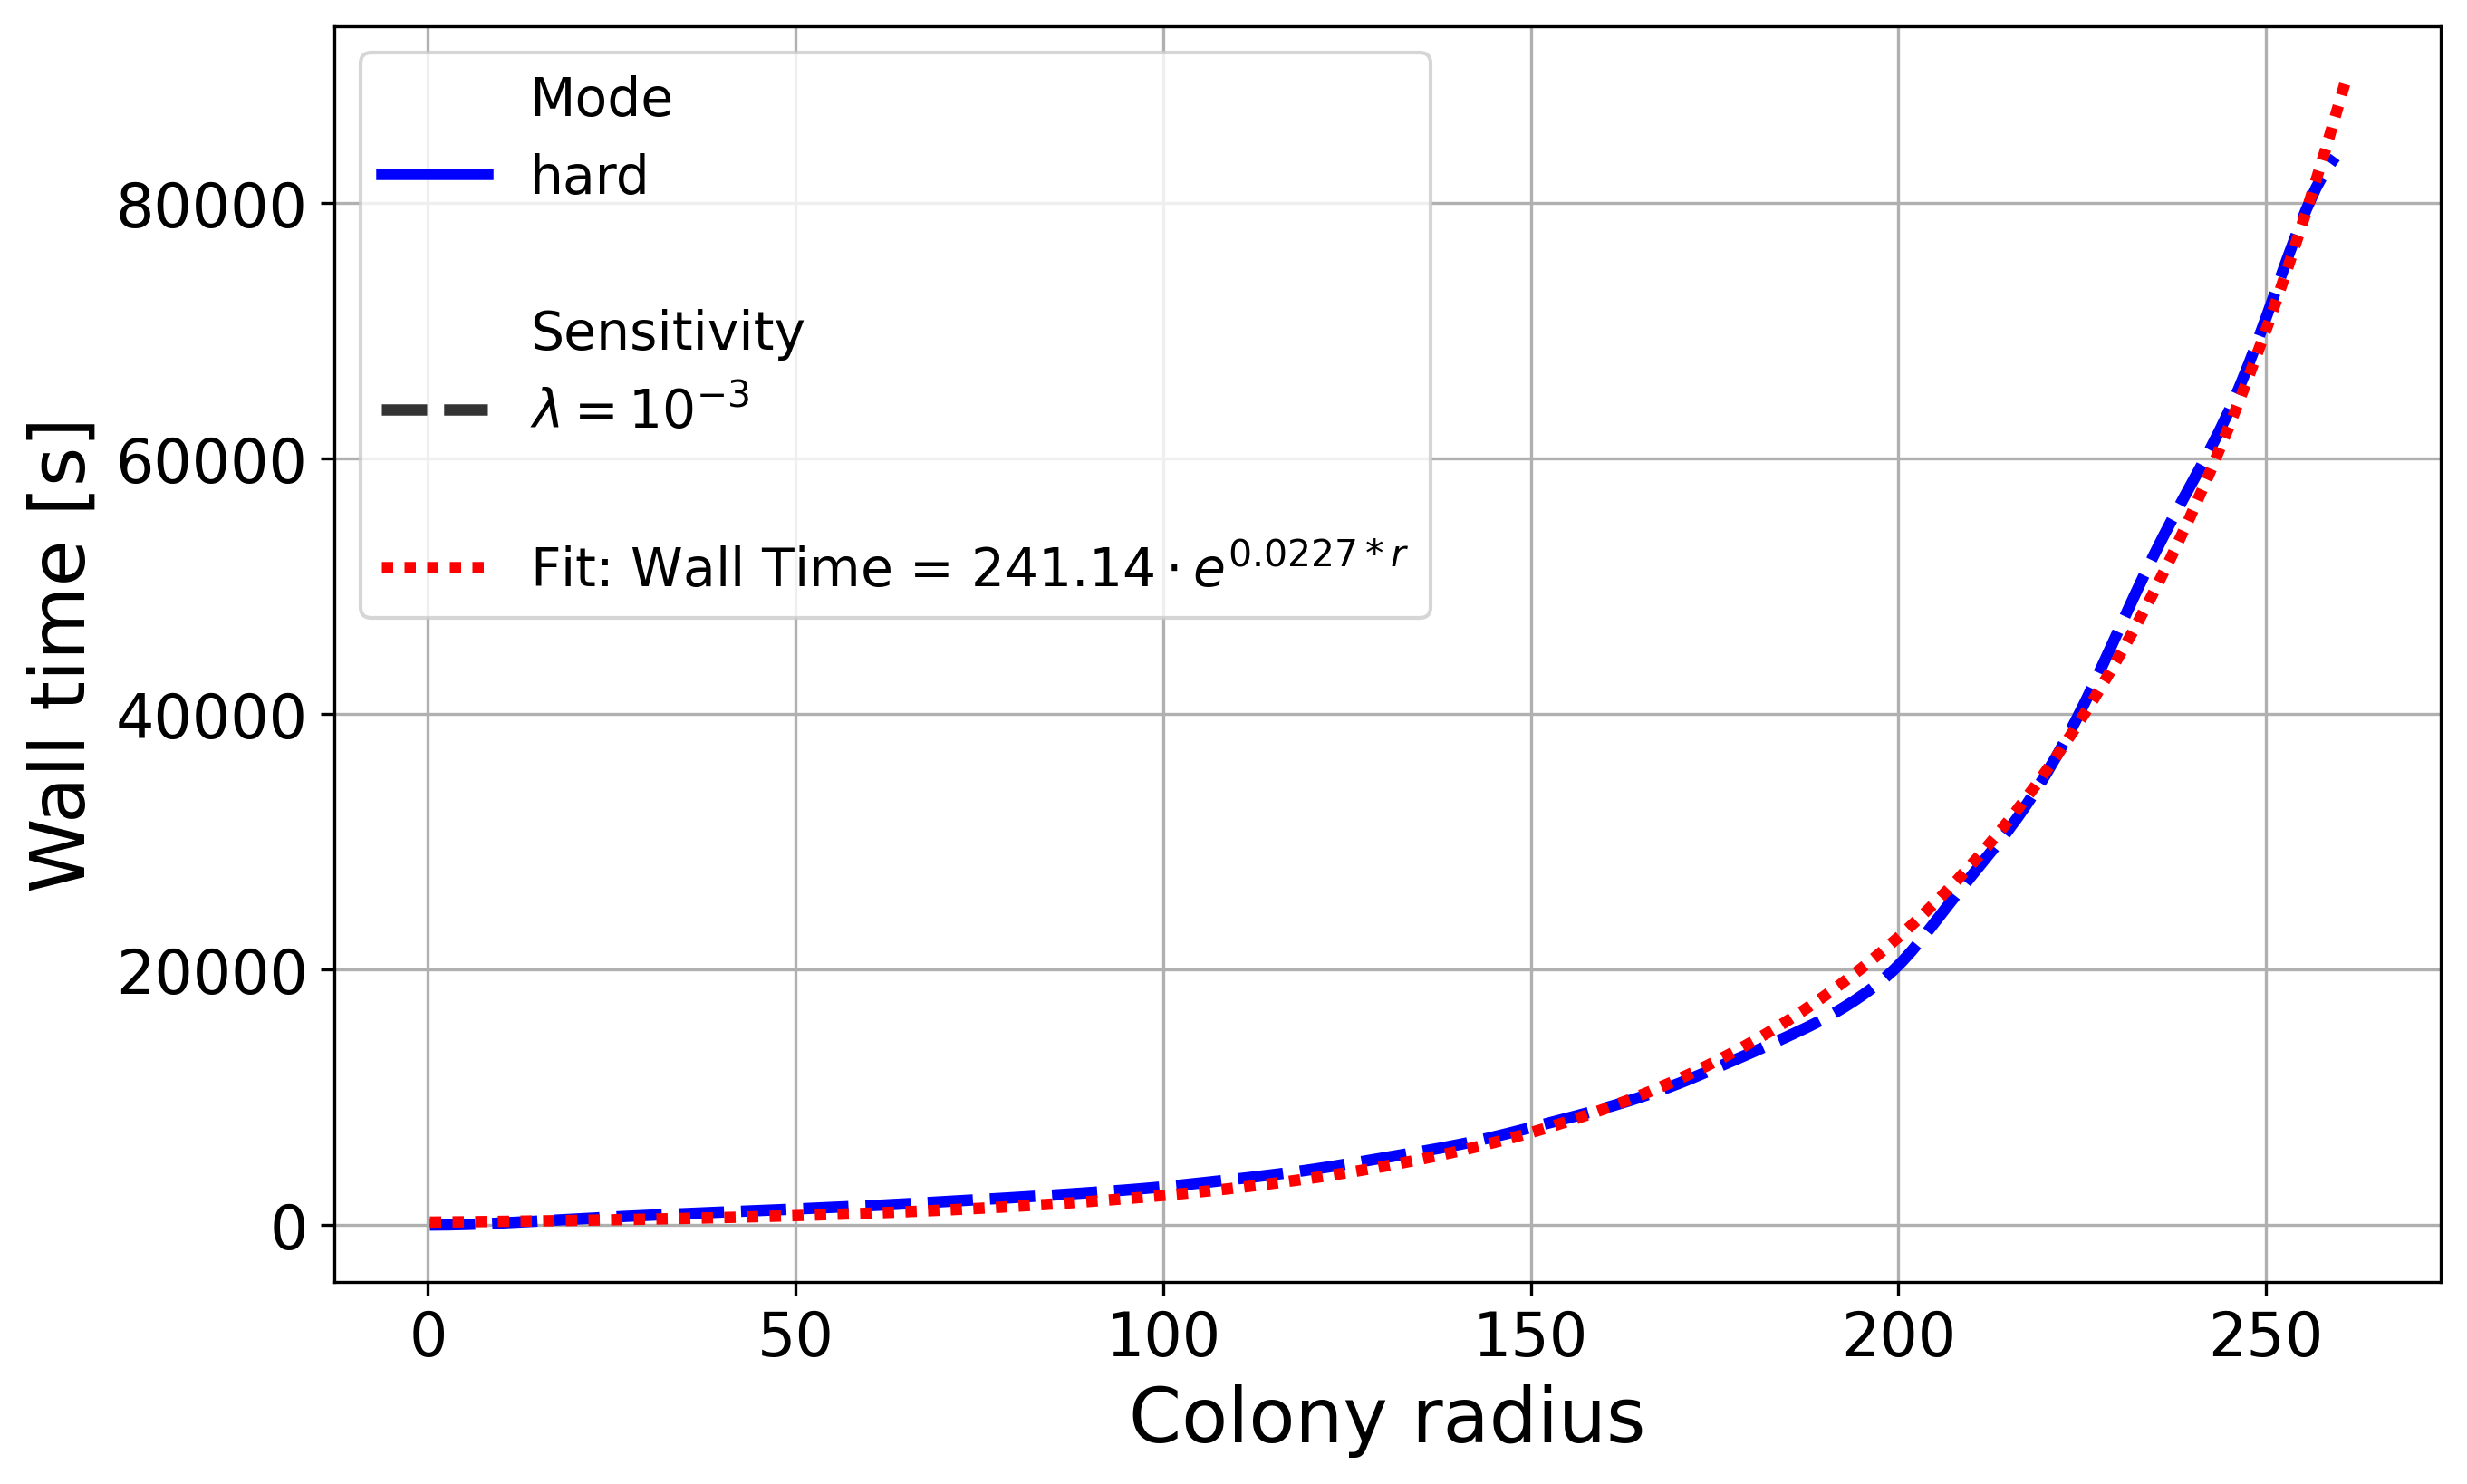
\includegraphics[width=\textwidth]{figures/figures_paper/huge/huge_wall_time_vs_radius_with_fit.png}
%             \end{figure}
%         \end{column}

%     \end{columns}

% \end{frame}

\begin{frame}
    \frametitle{Largest Colony: R = 260, 301k cells, 24h@112 cores}



    \begin{center}
        {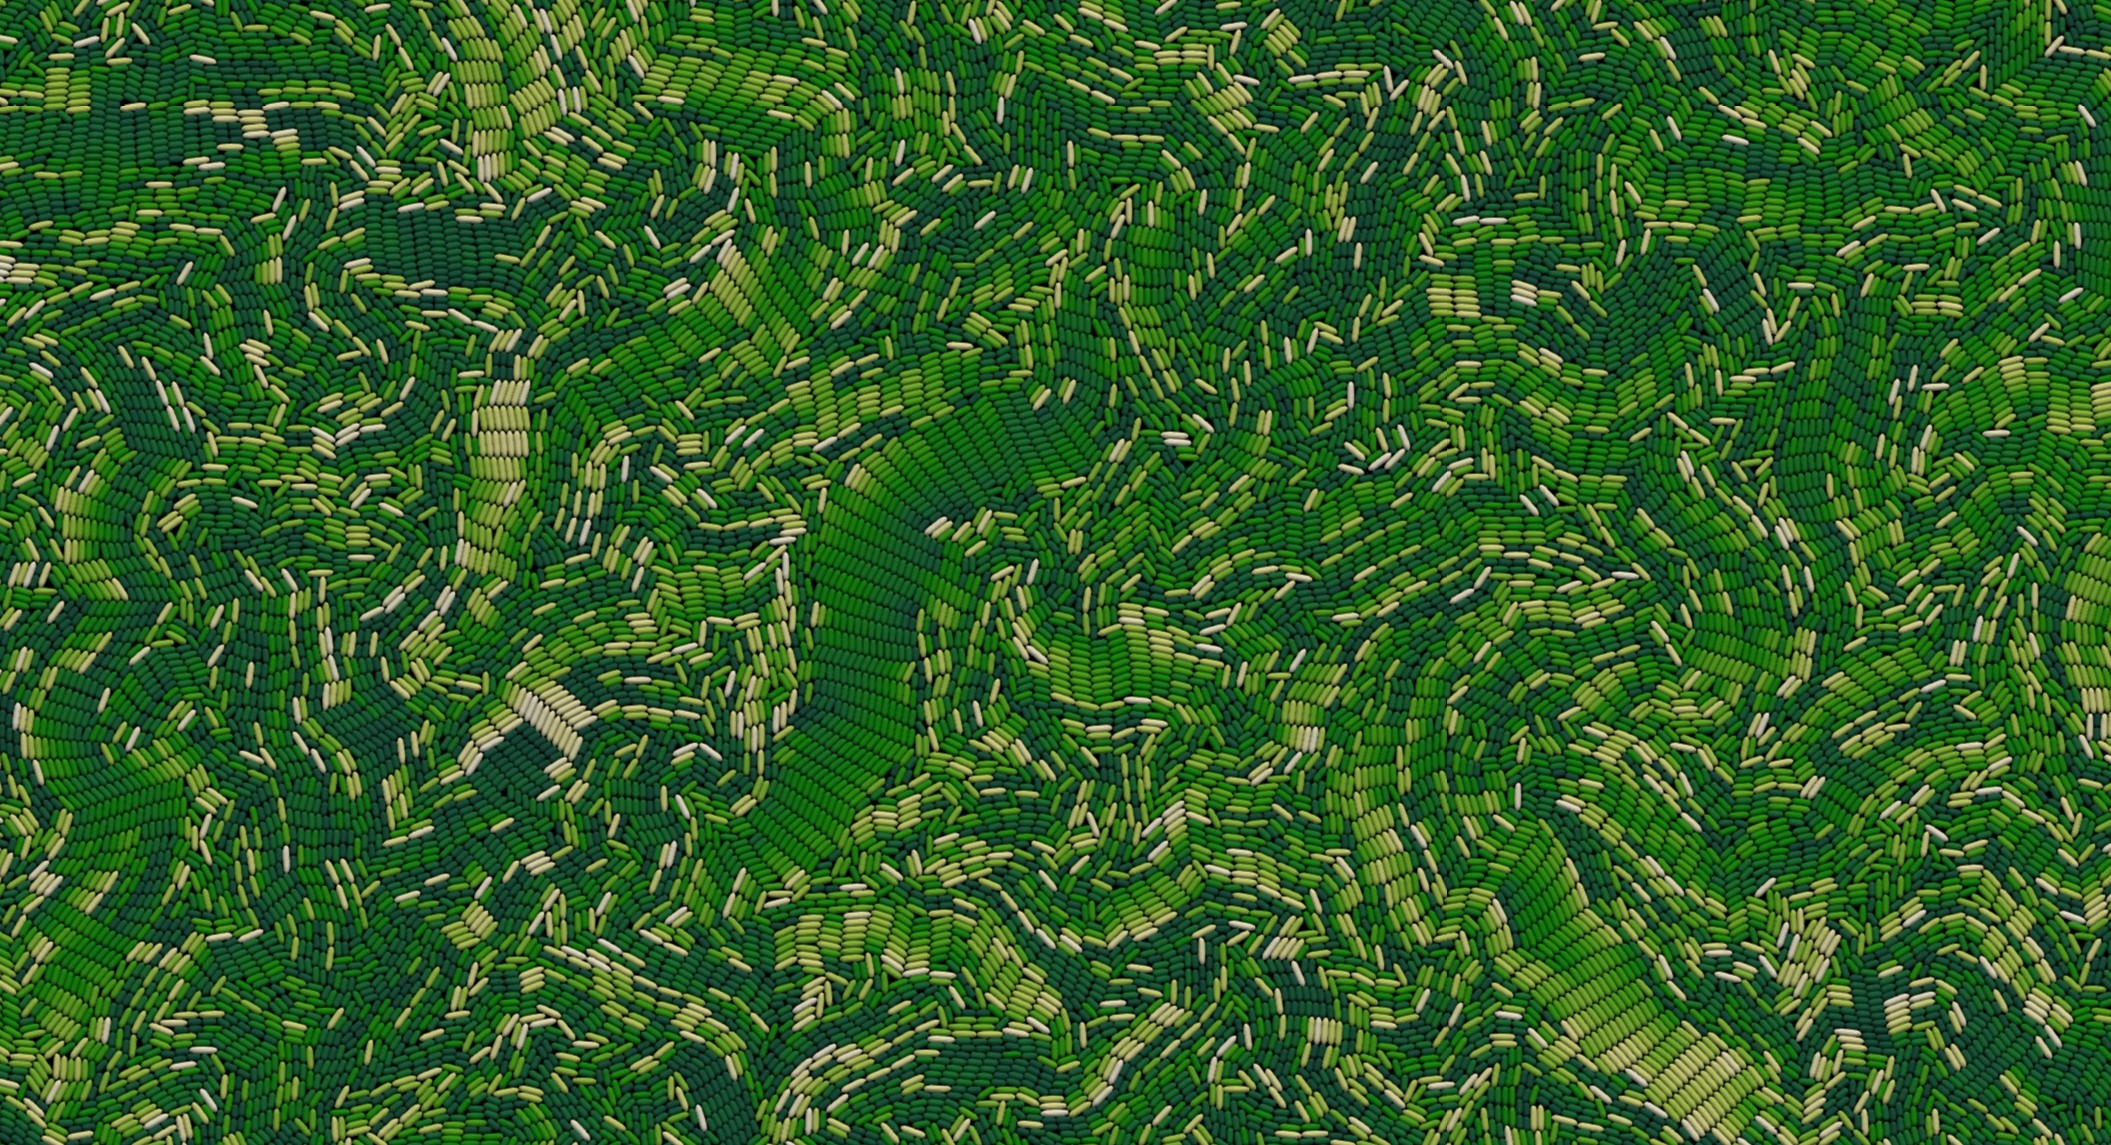
\includegraphics[width=0.9\textwidth]{figures/figures_paper/huge/huge_cropped.jpeg}}\\[0.6em]
        \small
        \href{https://home.cit.tum.de/~ler/bacteria/videos/huge_high_quality.jpeg}{\textcolor{blue}{{View Full Image}}}
    \end{center}
\end{frame}

% ============================================================
% SECTION 7: SYNTHESIS & CONCLUSIONS
% ============================================================

\section{Discussion}

% \begin{frame}
%     \frametitle{Model Comparison Summary}

%     \vspace{-0.5cm}
%     \begin{table}
%         \centering
%         \begin{tabular}{lcccc}
%                                               & \multicolumn{2}{c}{\textbf{Soft}} & \multicolumn{2}{c}{\textbf{Hard}}                                              \\
%             \cmidrule(lr){2-3} \cmidrule(lr){4-5}
%             \textbf{Criterion}
%                                               & \shortstack{Small                                                                                                  \\Colonies}
%                                               & \shortstack{Large                                                                                                  \\Colonies}
%                                               & \shortstack{Small                                                                                                  \\Colonies}
%                                               & \shortstack{Large                                                                                                  \\Colonies} \\
%             \midrule
%             \multicolumn{5}{l}{\textit{Biological Fidelity:}}                                                                                                      \\
%             $\quad$  Ring formation           & \cmark                            & \cmark                            & \cmark        & \cmark                     \\
%             $\quad$  Packing density          & \cmark                            & \xmark                            & \cmark        & \cmark                     \\
%             $\quad$  Microdomain quality      & \cmark                            & \xmark                            & \cmark        & \cmark                     \\
%             \midrule
%             \multicolumn{5}{l}{\textit{Performance:}}                                                                                                              \\
%             $\quad$ Runtime                   & \cmark \cmark                     & \xmark \xmark \textup{*}          & \cmark        & \cmark \cmark              \\
%             $\quad$ Parallel scalability      & $\sim$                            & \cmark \cmark \textup{*}          & $\sim$        & \cmark \cmark              \\
%             $\quad$ Implementation complexity & \cmark \cmark                     & \cmark \cmark                     & \emoji{skull} & \emoji{skull}\emoji{skull} \\
%         \end{tabular}
%     \end{table}

%     \vspace{0.3cm}
%     \footnotesize{\textup{*} Actual soft model performance degrades significantly due to timestep reduction.}

% \end{frame}

\begin{frame}
    \frametitle{When to use each Model?}

    \vspace{-0.55cm}

    \begin{columns}
        \begin{column}{0.5\textwidth}
            \begin{alertblock}{Soft Model}
                \textbf{Use when:}
                \begin{itemize}
                    \item Exploring small Colonies
                    \item Macroscopic effects matter
                \end{itemize}

                \textbf{Advantages:}
                \begin{itemize}
                    \item Simple implementation
                    \item Can model "squishy" bacteria
                \end{itemize}

                \textbf{Disadvantages:}
                \begin{itemize}
                    \item Slow simulations
                    \item Causes Artefacts
                \end{itemize}
            \end{alertblock}
        \end{column}
        \begin{column}{0.5\textwidth}
            \begin{exampleblock}{Hard Model }
                \textbf{Use when:}
                \begin{itemize}
                    \item Exploring large Colonies
                    \item Cell-scale phenomena matter
                \end{itemize}

                \textbf{Advantages:}
                \begin{itemize}
                    \item Faster simulations
                    \item Physical accuracy
                \end{itemize}

                \textbf{Disadvantages:}
                \begin{itemize}
                    \item Complex implementation
                    \item[]
                \end{itemize}
            \end{exampleblock}
        \end{column}

    \end{columns}

\end{frame}

% ============================================================
% SECTION 8: FUTURE WORK
% ============================================================

\section{Future Directions}

\begin{frame}
    \frametitle{Future Work}

    \begin{enumerate}
        \item \textbf{Hard Model Solver Improvements}
              \begin{itemize}
                  \item Leverage PETSc GPU support
                  \item Warm-start BBPGD with previous solution
              \end{itemize}

              \vspace{0.3cm}

        \item \textbf{Soft Model Enhancements}
              \begin{itemize}
                  \item Consider overlap, in adaptive timestepping.
                  \item Consider alternatives that prevent overlap
                  \item Slow down cell growth (globally) on overlap?
              \end{itemize}

              \vspace{0.3cm}

        \item \textbf{More Biological Applications}
              \begin{itemize}
                  \item Other cell shapes (soft bodies?)
                  \item More complex models (Nutrient fields?, Outside forces?)
                  \item Utilize 3D capabilities
              \end{itemize}
    \end{enumerate}

\end{frame}

% ============================================================
% CONCLUSIONS
% ============================================================

\section*{Conclusions}

\begin{frame}
    \begin{center}
        \vspace{1cm}
        {\LARGE \textbf{Thank you for your attention!}}

        \vspace{1.5cm}

        \Huge{Questions?}

        \vspace{.8cm}

        \small
        \texttt{manuel.lerchner@tum.de}

        \vspace{0.3cm}
        Code: \url{https://github.com/manuellerchner/MicrobeGrowthSim-IDP}

        \vspace{0.2cm}
        Supplementary materials: \url{https://home.cit.tum.de/~ler/bacteria/}
    \end{center}
\end{frame}

\begin{frame}[allowframebreaks, noframenumbering]
    \frametitle{References}
    \scriptsize
    \bibliographystyle{apalike}
    \bibliography{../latex/literature}
\end{frame}

\appendix

\begin{frame}
    \frametitle{Backup: CFL vs. Runtime and Constraints}

    \begin{figure}
        \centering
        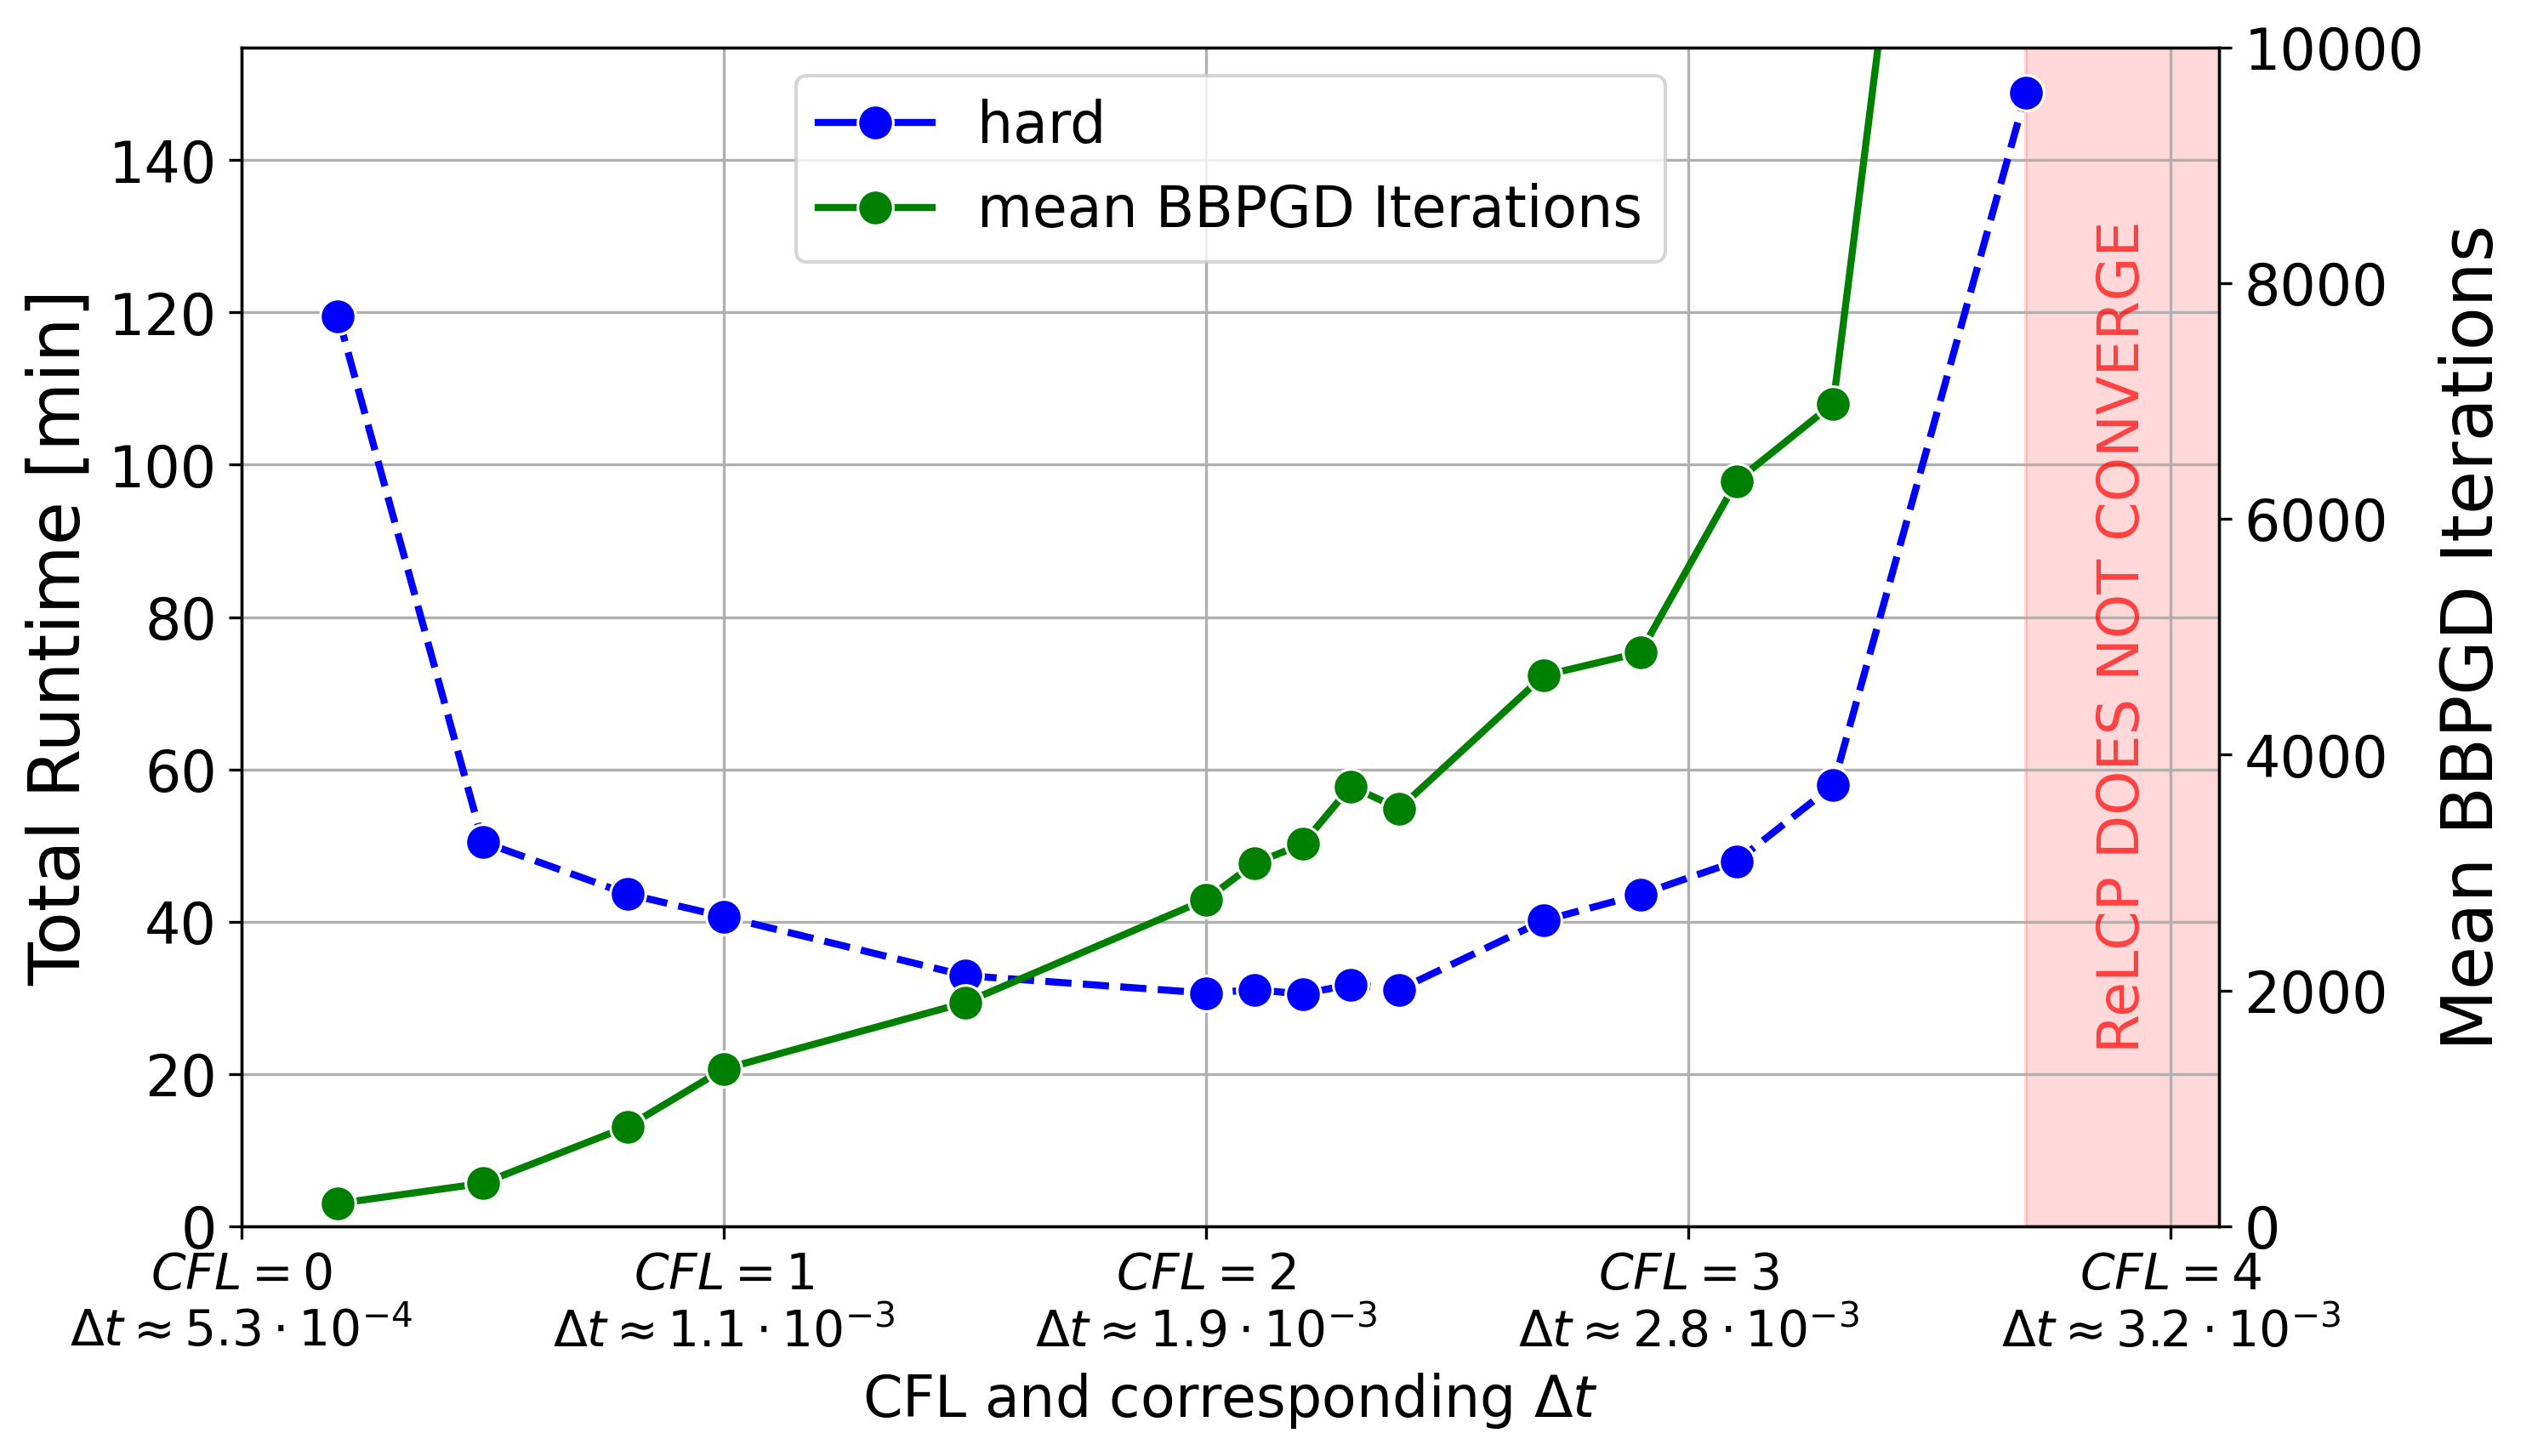
\includegraphics[width=0.8\textwidth]{figures/figures_paper/bbpgd/cfl_vs_runtime_and_constraints.png}
    \end{figure}
\end{frame}

\begin{frame}
    \frametitle{Backup: BBPGD Iterations vs. Number of Particles}

    \begin{figure}
        \centering
        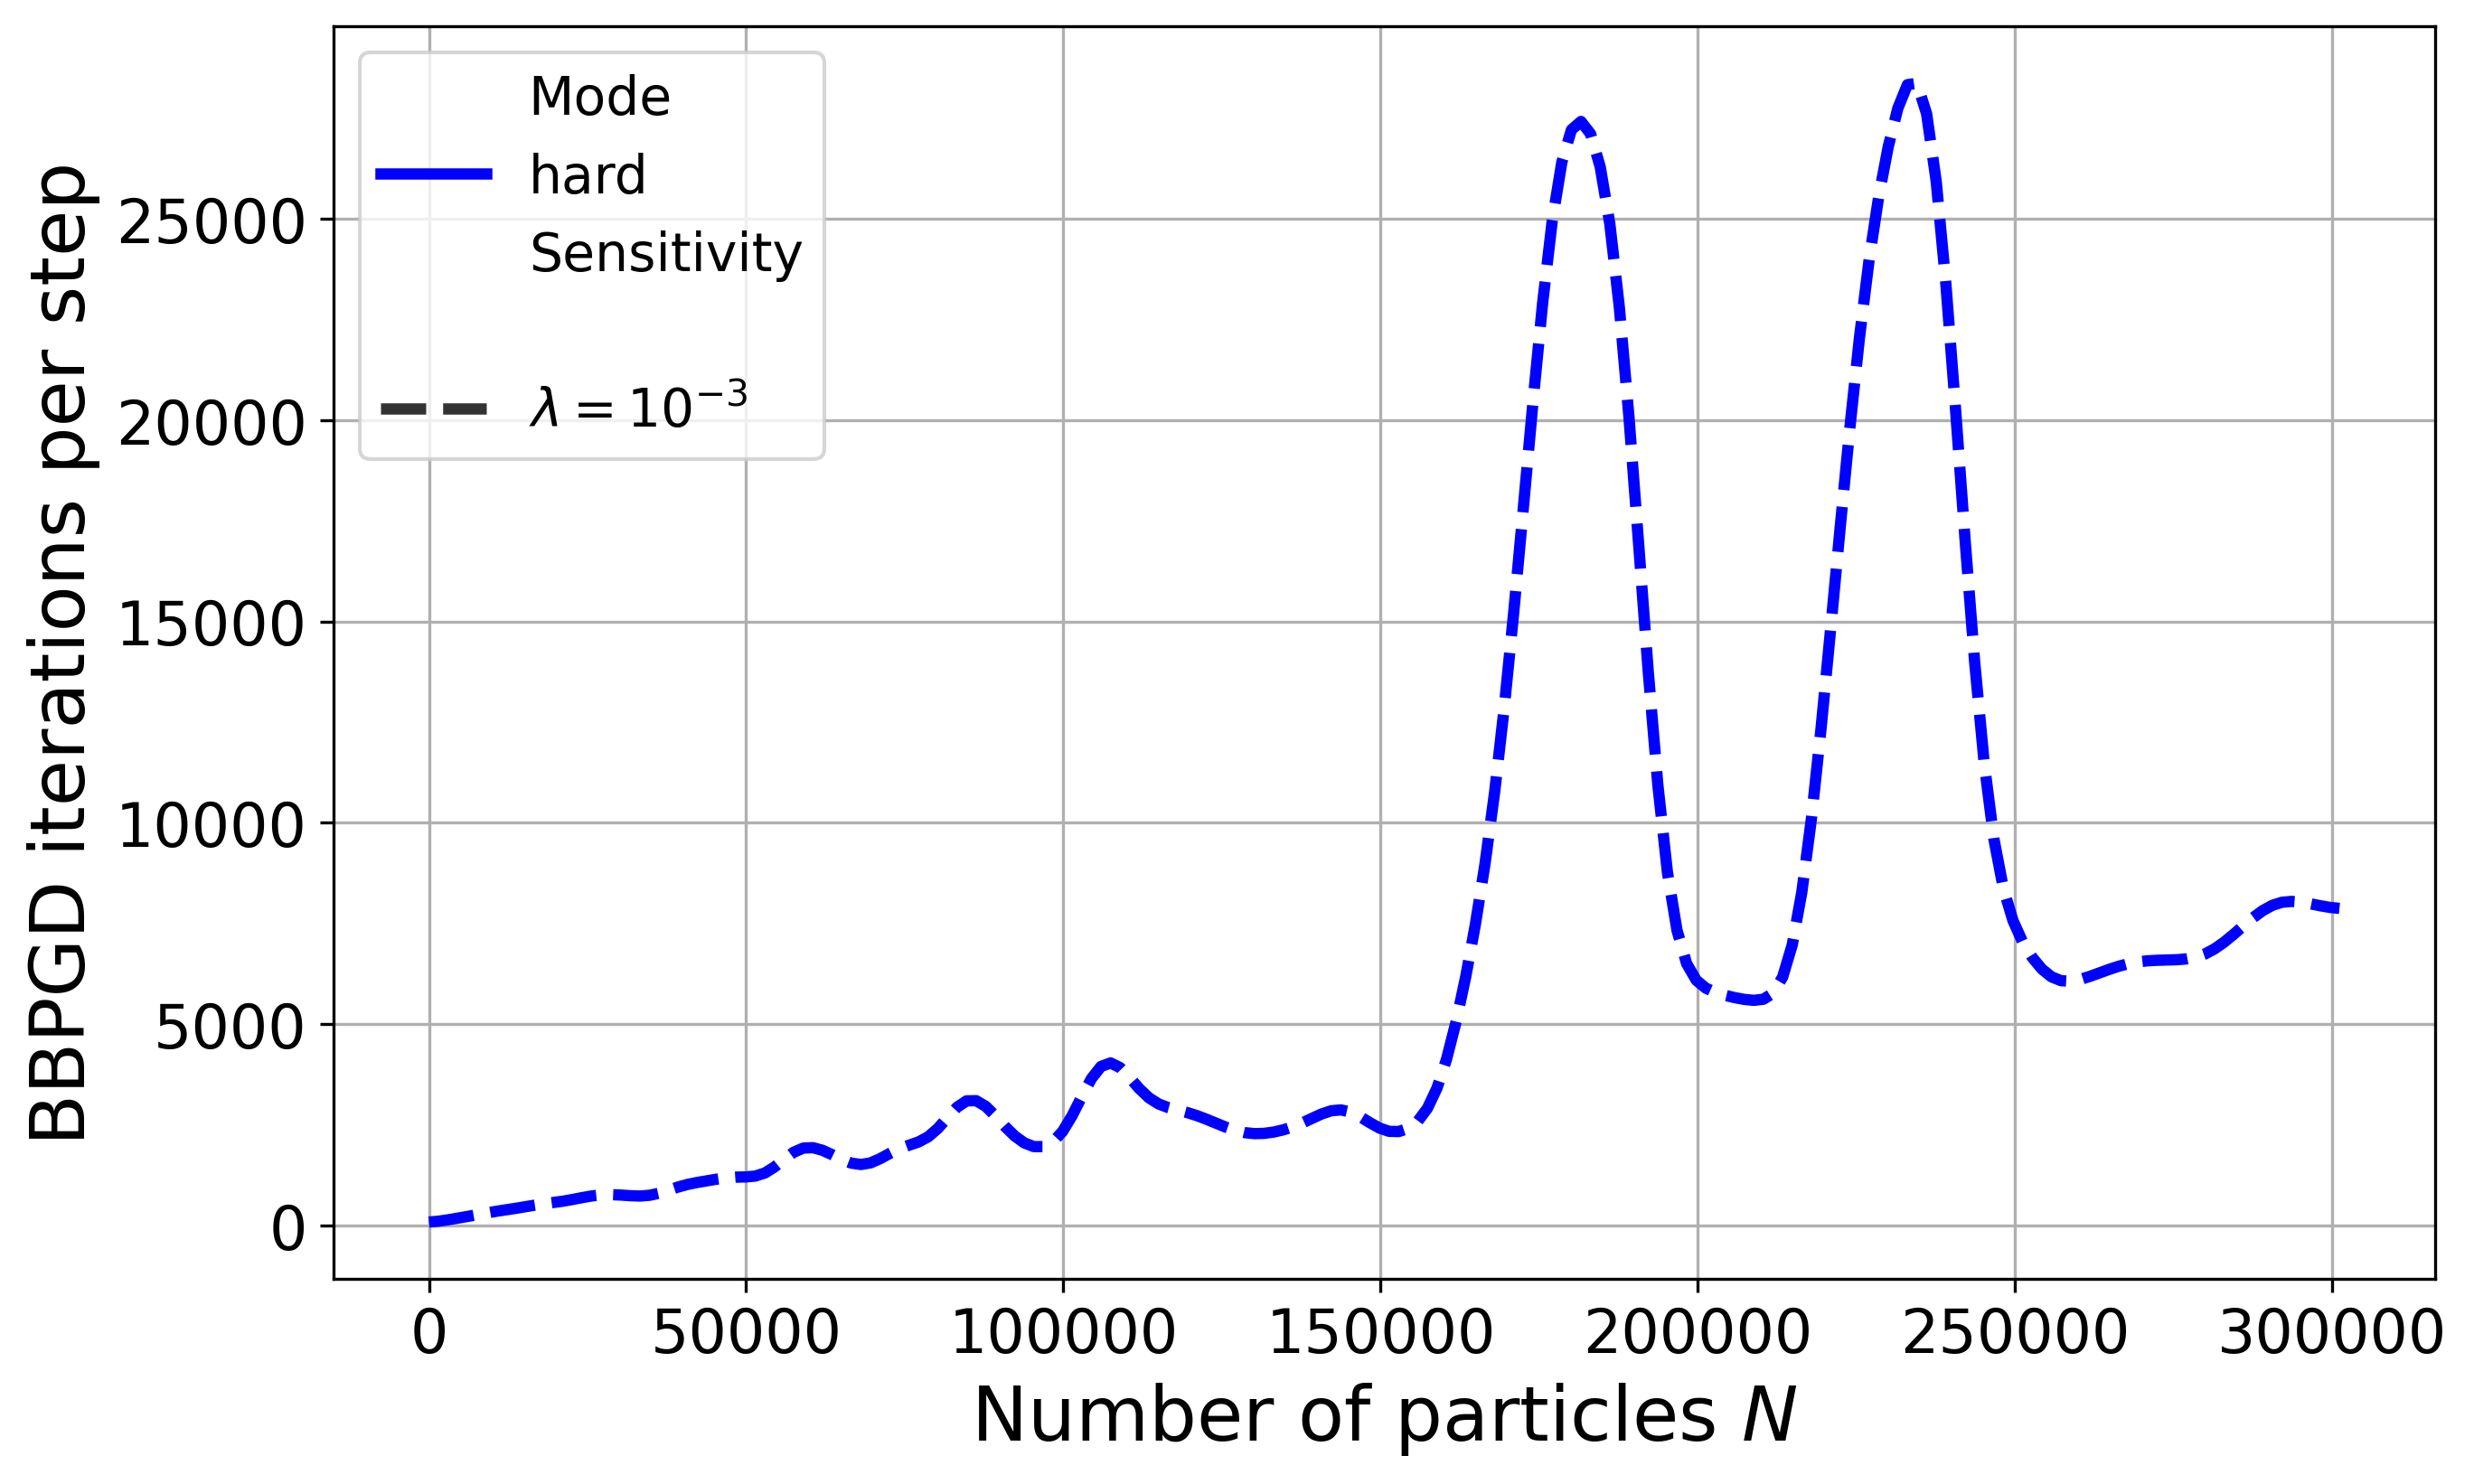
\includegraphics[width=0.8\textwidth]{figures/figures_paper/huge/huge_bbpgd_iterations_per_step_vs_num_particles.png}
    \end{figure}
\end{frame}

\end{document}